\pdfobjcompresslevel 0
%%%%%%  %%%%%%  %%%%%%  \\\\\\\  Set Print  ////////////////
\def\print{1}
\if\print1
    \newcommand\open{openright}
    \newcommand\toPrint{\clearpage{\pagestyle{empty}\cleardoublepage}}
    \newcommand\reliure{.75cm}
    \newcommand\locHead{RO,LE}
    \newcommand\version{print version}
\else
    \newcommand\open{openany}
    \newcommand\toPrint{\clearpage}
    \newcommand\reliure{0cm}
    \newcommand\locHead{R}
    \newcommand\version{digital version}
\fi
%%%%%%  %%%%%%  %%%%%%  %%%%%%  %%%%%%  %%%%%%  %%%%%%  %%%%%%  %%%%%%  %%%%%% 

%%%%%%  %%%%%%  %%%%%%  \\\\\\\  Set Doc  ////////////////
\documentclass[12pt,twoside,a4paper,french,\open]{report}
\usepackage{morewrites} % need to make more \listof{}
\usepackage[left=2.5cm,right=2.5cm,top=2.42cm,bottom=2.42cm,includeheadfoot]{geometry}
\addtolength{\evensidemargin}{-\reliure}
\addtolength{\oddsidemargin}{+\reliure}
%%%%%%  %%%%%%  %%%%%%  %%%%%%  %%%%%%  %%%%%%  %%%%%%  %%%%%%  %%%%%%  %%%%%% 

%%%%%%  %%%%%%  %%%%%%  \\\\\\\  Set lang  ////////////////
\usepackage[utf8]{inputenc}
\usepackage[french]{babel}
\usepackage{eurosym}
\usepackage[T1]{fontenc}
%%%%%%  %%%%%%  %%%%%%  %%%%%%  %%%%%%  %%%%%%  %%%%%%  %%%%%%  %%%%%%  %%%%%% 

%%%%%%  %%%%%%  %%%%%%  \\\\\\\  Set style  ////////////////

%%%%%%  Set fig tab cod  ////////////////
\usepackage{graphicx}
\usepackage{svg}
\usepackage{multicol}
\usepackage{wrapfig}
\usepackage{subcaption}
\newcounter{subcode}
\renewcommand{\thesubcode}{\alph{subcode}}
\usepackage[procnames,final]{listings}
\lstdefinelanguage{LDA}{
    basicstyle=\ttfamily,        
    morestring=[b][\color{black}]",
    morekeywords=[1]{If, Then, Else, End, For, While, do},
    keywordstyle=[1]{\color{red}\bfseries},
    morekeywords=[2]{in},
    keywordstyle=[2]{\color{red}},
    morekeywords=[3]{start, end, interval},
    keywordstyle=[3]{\color{blue}},
}
\lstset{language=Python, 
    basicstyle=\ttfamily\small,
    breaklines=true,
    keywordstyle=\color{keywords},
    commentstyle=\color{comments},
    stringstyle=\color{py-red},
    showstringspaces=false,
    identifierstyle=\color{py-green},
    procnamekeys={def,class},
    literate={à}{{\`a}}1 {é}{{\'e}}1 {è}{{\`e}}1 {ê}{{\^e}}1 }
\lstdefinelanguage{json}{
    basicstyle=\ttfamily\small,
    showstringspaces=false,
    breaklines=true,
    identifierstyle=\color{black},
    literate=
     *{0}{{{\color{numb}0}}}{1}
      {1}{{{\color{numb}1}}}{1}
      {2}{{{\color{numb}2}}}{1}
      {3}{{{\color{numb}3}}}{1}
      {4}{{{\color{numb}4}}}{1}
      {5}{{{\color{numb}5}}}{1}
      {6}{{{\color{numb}6}}}{1}
      {7}{{{\color{numb}7}}}{1}
      {8}{{{\color{numb}8}}}{1}
      {9}{{{\color{numb}9}}}{1}
      {:}{{{\color{punct}{:}}}}{1}
      {,}{{{\color{punct}{,}}}}{1}
      {\{}{{{\color{delim}{\{}}}}{1}
      {\}}{{{\color{delim}{\}}}}}{1}
      {[}{{{\color{delim}{[}}}}{1}
      {]}{{{\color{delim}{]}}}}{1},
}
%%%%%%  Set page  ////////////////
\usepackage{fancyhdr}
\usepackage{sectsty}
\usepackage{titlesec}
\usepackage{setspace}
\setlength{\abovedisplayshortskip}{0.1cm}
\setlength{\belowdisplayshortskip}{0.1cm}
\setlength{\abovedisplayskip}{0.1cm}
\setlength{\belowdisplayskip}{0.1cm}
\setlength{\belowcaptionskip}{-5pt}
\renewcommand\thepage{\arabic{page}}
%%%%%%  set margin  ////////////////
\def\changemargin#1#2{\list{}{\rightmargin#2\leftmargin#1}\item[]}
\let\endchangemargin=\endlist 
%%%%%%  Set par  ////////////////
\titlespacing{\paragraph}{2\parindent}{0.75\parindent plus .2ex minus 2ex}{\parindent plus .2ex}
\titleformat*{\paragraph}{\normalsize\bfseries\scshape}
\titlespacing{\subparagraph}{\parindent}{\parskip}{1ex plus .2ex}
\titleformat*{\subparagraph}{\small\scshape}
%%%%%%  Set font  ////////////////
%default Font
\usepackage{libertine}
\usepackage{libertinust1math}
%number page
\newcommand\pageFont{\fontfamily{pzc}\selectfont\itshape\large\vspace{0.25cm}}
%introduction
\newcommand\introFont{
    \setstretch{1,28}
    \fancyhead[\locHead]{\textsc{Introduction}}
}
%dedicace
\newcommand\dediFont{\fontfamily{augie}\selectfont\setstretch{1,6}\centering}
%citation
\newcommand\citFont{\fontfamily{bch}\selectfont}
%resumé de chap
\newcommand\resFont{\setstretch{1,42}\setlength{\parindent}{20pt}\setlength{\parskip}{7pt}\itshape\large}
%conclu de part
\newcommand\conFont{
    \pagestyle{myFancy}
    \fancyhead{}
    \fancyhead[\locHead]{\footnotesize{\textsc{Partie~\thepart~~---~~Conclusion}}}
    \setstretch{1,36}\setlength{\parindent}{20pt}\setlength{\parskip}{5pt}
}  
% question intro
\newcommand\QR[1]{\par\vspace{0.1cm}{\bfseries\itshape\hspace{.75\parindent}\gui{#1~?}}\vspace{0.15cm}\par}
%sous chap
\newcommand\subchapFont{
    \titleformat{\section}[hang]
        {\toPrint\vspace{15pt}\flushright\huge\bfseries}
        {Sous-chapitre \arabic{chapter}.\includegraphics[width=0.7cm]{Figures/fontNumber/\arabic{section}.pdf}}
        {0pt}
        {\break\scshape}
}
%discussion
\newcommand\discuFont{
    \clearpage
    \pagestyle{empty}
    \renewcommand\myChapter[3][]{
        \ifx&##1&
            \chapter[##2##3]{\textsc{\lowercase{##2}##3}~~}
        \else
            \chapter[##2##1]{\textsc{\lowercase{##2}##3}~~}
        \fi
        \label{chap:\thepart-\thechapter}
        \vspace{-0.85cm}
    }
    \renewcommand{\chaptertitlename}{Élément}
    \titleformat{\chapter}[display]
        {\vspace{-2.5cm}\raggedleft\Huge\bfseries}
        {\chaptertitlename~\includegraphics[width=0.7cm]{Figures/fontNumber/\thechapter.pdf}~~}
        {0pt}
        {\raggedleft\huge\bfseries\scshape}
}
%conclu
\newcommand\concluFont{
    \pagestyle{myFancy}
    \fancyhead{}
    \fancyhead[\locHead]{\textsc{Conclusion et Perspectives}}
}
%annexe
\newcommand\annexeFont{
    \setcounter{section}{0}
    \titleformat{\section}[hang]{\flushleft\bfseries}{\thesection~~}{0pt}{}
    \titleformat{\subsection}[hang]{\flushleft\bfseries}{\thesubsection~}{0pt}{}
    \renewcommand{\thesection}{\Roman{section}}
    \renewcommand{\thesubsection}{\Roman{section}. \Roman{subsection}}
    \mtcsetoffset{minitoc}{0pt}
    \setlength{\mtcindent}{24pt}
}
%%%%%%  MyDefautStyle  ////////////////
\newcommand\myDefautStyle{\setstretch{1,26}\setlength{\parindent}{15pt}}
\let\defaultHrule\headrulewidth
\fancypagestyle{plain}{
    \fancyhf{}
    \fancyfoot[C]{\pageFont\thepage}
    \renewcommand{\headrulewidth}{0pt}
}
\fancypagestyle{myFancy}{
    \fancyhf{}
    \fancyhead[RO]{\footnotesize{\textsc{PARTIE~\thepart~~---~~CHAPITRE~\thechapter.}}}
    \fancyhead[LE]{\footnotesize{\Roman{part}.\rightmark}}
    \renewcommand{\headrulewidth}{\defaultHrule}
    \fancyfoot[\locHead]{\pageFont\thepage}
}

%%%%%%  MyItemStyle  ////////////////
\newcommand\myItemStyle{\setstretch{1,0}\setlength{\parindent}{0pt}}
\usepackage{enumitem}
\renewcommand{\FrenchLabelItem}{\textbullet}
\setlist[itemize]{leftmargin=*}
\setlist[enumerate]{leftmargin=*}%noitemsep,
%%%%%%  MyPhantom  ////////////////
\newcommand\myPhantom[2]{\phantomsection\addcontentsline{toc}{#1}{#2}}
%%%%%%  MyPart  ////////////////
\titleformat{\part}[display]
    {\fontsize{35}{42}\selectfont\filcenter\bfseries}
    {\partname{} \thepart}
    {0em}
    {}
\newcommand\myPart[1]{
    \clearpage
    \pagestyle{empty}
    \part{#1}
    \myDefautStyle
}
%%%%%%  MyChapter  ////////////////
\titleformat{\chapter}[display]
    {\raggedleft\fontsize{30}{38}\selectfont\bfseries}
    {\chaptertitlename~\includegraphics[width=1cm]{Figures/fontNumber/\thechapter.pdf}~~}
    {20pt}
    {\raggedleft\fontsize{28}{30}\selectfont\bfseries\scshape}
\newcommand\myChapter[3][]{
    \clearpage
    \pagestyle{empty}
    \ifx&#1&
        \chapter[#2#3]{\textsc{\lowercase{#2}#3}~~}
    \else
        \chapter[#2#1]{\textsc{\lowercase{#2}#3}~~}
    \fi
    \label{chap:\thepart-\thechapter}
    \setstretch{1,1}
    \minitoc
    \toPrint
    \pagestyle{myFancy}
    \myDefautStyle
}
%%%%%%  MyResum  ////////////////
\newenvironment{resumChap}[1][.84]{%
    \pagestyle{plain}
    \vspace{2.42cm}\strut\newline
    {\fontsize{28}{40}\selectfont\bfseries\itshape Résumé}
    \myPhantom{paragraph}{Résumé}
    \vspace{1.42cm}\newline
    \strut\hfill
    \begin{minipage}{#1\linewidth}
    \resFont
}{%
    \end{minipage}
    \hfill\strut
    \toPrint
}
%%%%%%  MyConclu  ////////////////
\usepackage{fmtcount}
\newenvironment{concluPart}{%
    \clearpage
    \pagestyle{empty}
    \chapter*{\vspace{1cm}Conclusion\\ de la \ordinalstring{part}[f] partie}
    \addstarredchapter{\texorpdfstring{\hfill\textit{Conclusion Partie \thepart~~~~}}{Conclusion Partie \thepart}}\label{chap:\thepart-0}
    \toPrint
    \conFont
}{%
    \clearpage
}
%%%%%%  NoColorUrl  ////////////////
\newcommand\noColorHref[2]{\href{#1}{\textcolor{myBlack}{#2}}}
%%%%%%  %%%%%%  %%%%%%  %%%%%%  %%%%%%  %%%%%%  %%%%%%  %%%%%%  %%%%%%  %%%%%%  

%%%%%%  %%%%%%  %%%%%%  \\\\\\\  Set other  ////////////////

%%%%%%  PDF to Annexe  ////////////////
\usepackage{pdfpages}
\newcommand\PDFannexeOne[4][0.7]{\includepdf[frame,scale=#1,pages=1,pagecommand={#3\label{pdf:#2}}]{#4}}
\newcommand\PDFannexe[4][0.7]{
    \PDFannexeOne[#1]{#2}{#3}{#4}
    \includepdf[frame,width=\linewidth,pages=2-,pagecommand={}]{#4}
}
\newcommand\EuroGraph[2]{
    \phantomsection\pdfbookmark[paragraph]{#1}{#2}
    \vfill\noindent\footnotesize{#1}\newline\vspace{-0.2cm}
    ~
    \includegraphics[width=0.89\linewidth]{Annexe/euro382/#2.pdf}\label{#2}\\
}
%%%%%%  break url  ////////////////
\usepackage[hyphens]{url}
%%%%%%  Set clor  ////////////////
\usepackage{xcolor}
%text color
\definecolor{myBlack}{rgb}{0.042,0,0}
%background
\definecolor{antiflashColor}{rgb}{0.95, 0.95, 0.96}
%\newcommand\BackGroundColor{antiflashColor}
%links color
\definecolor{red-link}{rgb}{.42,0,0}
%url color
\definecolor{blue-url}{rgb}{0,0,.42}
%abr color
\definecolor{abr-color}{rgb}{0.36, 0.22, 0.33}
%cite color
\definecolor{red-cite}{rgb}{0.53, 0.15, 0.34}
%citation box color
\definecolor{box-gray}{rgb}{0.97, 0.97, 1.0}
\definecolor{text-gray}{gray}{0.17}
%python color
\definecolor{keywords}{RGB}{255,0,90}
\definecolor{comments}{RGB}{0,0,113}
\definecolor{py-red}{RGB}{160,0,0}
\definecolor{py-green}{RGB}{0,150,0}
%json color
\colorlet{punct}{red!60!black}
\definecolor{delim}{RGB}{20,105,176}
\colorlet{numb}{magenta!60!black}
%%%%%%  %%%%%%  %%%%%%  %%%%%%  %%%%%%  %%%%%%  %%%%%%  %%%%%%  %%%%%%  %%%%%%

%%%%%%  %%%%%%  %%%%%%  \\\\\\\  Set hyper ref  ////////////////
\usepackage{hyperref}
\hypersetup{
  pdfauthor     = {Thibault DESPREZ},
  pdftitle      = {T.DESPREZ, Manuscrit de Th\`ese (\version)},
  pdfsubject    = {Conception et \'evaluation de kits robotiques p\'edagogiques.},
  pdfkeywords   = {Robotics Kit, Robot, Poppy, ErgoJr, Visual Programming, Snap!, Python, Digital Science},
  pdfproducer   = {Latex (compiled \today)},
  pdfcreator    = {pdflatex},
  bookmarksopen = false,
  bookmarksdepth= 10,
  linkcolor     = red-link,
  breaklinks    = true,
  citecolor     = red-cite,
  urlcolor      = blue-url,
  final         = true,
  colorlinks
  }
%%%%%%  %%%%%%  %%%%%%  %%%%%%  %%%%%%  %%%%%%  %%%%%%  %%%%%%  %%%%%%  %%%%%%  

%%%%%%  Set section  //////////////// after hyperref!
\makeatletter
\@addtoreset{chapter}{part}
\@addtoreset{footnote}{page}
\@addtoreset{subcode}{page}
\makeatother
%%%%%%  %%%%%%  %%%%%%  %%%%%%  %%%%%%  %%%%%%  %%%%%%  %%%%%%  %%%%%%  %%%%%%

%%%%%%  %%%%%%  %%%%%%  \\\\\\\  Set other  ////////////////

%%%%%%  Set PDF table  ////////////////
\usepackage[numbered]{bookmark}

%%%%%%  bib url annexe  ////////////////
\usepackage{multibib}
\newcites{Url}{Webographie}

%%%%%%  MyCite  ////////////////
%bib
\newcommand\citeB[1]{{\footnotesize\cite{#1}}}
%url
\newcommand\citeURL[1]{{\footnotesize\citeUrl{#1}}}
%annexe
\newcommand\citeA[1]{{\footnotesize(\textit{cf.}~\textsc{Annexe}~\ref{#1}, \textit{p.}\pageref{#1})}} 
%figure
\newcommand\citeF[1]{{\footnotesize(\textit{cf.}~\textsc{Figure}~\ref{#1}, \textit{p.}\pageref{#1})}} 
%table
\newcommand\citeT[1]{{\footnotesize(\textit{cf.}~\textsc{Table}~\ref{#1}, \textit{p.}\pageref{#1})}} 
%code
\newcommand\citeC[1]{{\footnotesize(\textit{cf.}~\textsc{Prog.}\ref{#1}, \textit{p.}\pageref{#1})}}
%section
\newcommand\citeS[1]{{\footnotesize(\textit{cf.}~\textsc{Section}~\ref{#1}, \textit{p.}\pageref{#1})}}
%rapport interne
\newcommand\citeR[1]{#1~\acrshort{RI}}
%question - in - part3chap3 euro382
\newcommand\citeQ[1]{{\footnotesize(\textit{q.}#1, page~\pageref{QA#1})}}  

%%%%%%  Set glossaries  ////////////////
\usepackage[acronym]{glossaries}
\newglossary[cit]{citation}{gls}{glo}{citation}
\makeglossaries
\setacronymstyle{short-long}
\renewcommand{\glstextformat}[1]{\textcolor{myBlack}{#1}}
\renewcommand{\acronymfont}[1]{\textcolor{abr-color}{#1}}
\newcommand\CapAcro[1]{\textcolor{abr-color}{\scshape#1}}
%abreviation
\loadglsentries{Bib/glossaries.tex}
\newglossarystyle{mystyleAcr}{
    \setglossarystyle{list}%
    \renewcommand*{\glossentry}[2]{%
    \raggedleft\setstretch{0,9}\item[\glsentryitem{##1}%
    \glstarget{##1}{\glossentryname{##1}}].\dotfill
    {\small\glossentrydesc{##1}\glspostdescription}\\{\scriptsize\textit{Présent en page(s):~}##2}\vspace{0.142cm}}%
}
%citation
\loadglsentries{Bib/citation.tex}
\newglossarystyle{mystyleCit}{
    \setglossarystyle{list}
    \renewcommand*{\glossentry}[2]{
    \raggedleft\item[\glsentryitem{##1}
    \glstarget{##1}{\glossentryname{##1}}]
    \glossentrysymbol{##1}~\dotfill~##2~}
}

%%%%%%  MyCitation  ////////////////
\usepackage[most]{tcolorbox}
\newtcolorbox{tcbremark}{
  breakable,
  enhanced jigsaw,
  oversize,
  rightrule     = 0pt,
  toprule       = 0pt,
  bottomrule    = 0pt,
  colback       = box-gray,
  arc           = 4pt,
  outer arc     = 0pt,
  title         = {},
  title style   = {white},
  fonttitle     = \color{myBlack}\bfseries,
  titlerule     = 0pt,
  bottomtitle   = 2pt,
  top           = 10pt,
  bottom        = 0pt,
  left          = 7pt,
}
\newcommand\citeAtion[1]{
  \vspace{-0.5cm}
  \begin{changemargin}{1.17cm}{\rightmargin}
    \begin{quotation}
      \begin{tcbremark}
        \color{text-gray}\setstretch{1,3}
        \citFont
        ~~~\og\textit{\glossentrydesc{#1}}~\fg~{\small\glsentrysymbol{#1}}
        \newline\glspl{#1}
        \vspace{0.142cm}\strut\hfill{\small ---~\glossentryname{#1}~---~}
      \end{tcbremark}
    \end{quotation}
  \end{changemargin}\par
}

%%%%%%  Table des codes  ////////////////
\usepackage{float}
\newfloat{code}{thp}{locod}
\floatname{code}{\textit{Prog.}}
\renewcommand{\thecode}{\thechapter.\arabic{code}~}

%%%%%%  Mini sommaire  ////////////////
\usepackage{minitoc}
\dominitoc
\setcounter{tocdepth}{1}
\setcounter{secnumdepth}{3}
\setcounter{minitocdepth}{2}

%%%%%%  MyRacourci  ////////////////
\usepackage{afterpage}
%%%%%%  MyCommand  ////////////////
%\citeB{label}      % cite bib
%\citeURL{label}    % cite url
%\citeF{label}      % cf figure
%\citeA{label}      % cf annexe
%\citeC{label}      % cf code
%\citeS{label}      % cf section
%\citeT{label}      % cf table
%\citeAtion{label}  % print citation text
%\nocite{*}         % cite all bib
%\gls{label}        % call abreviation
%\acrshort{label}   % call short abr
%\glsdesc{label}    % call long abr
%\siecle{num}       % call roman year
%\cf                % call \textit{cf.}
%\dico              % call \textit{d{\'e}f.}
%\AreF{flag}{text}  % need reread
%\comt{flag}{text}  % comment text
%\myL{}             % need to complet #TODO

%\PDFannexe[taille]{label}{name}{file}
%\PDFannexeOne[taille]{label}{name}{file}
%%%%%%  %%%%%%  %%%%%%  %%%%%%  %%%%%%  %%%%%%  %%%%%%  %%%%%%  %%%%%%  %%%%%%  


%%%%%%  raccourci  ////////////////
\renewcommand{\ier}{\up{ier}~}
\renewcommand{\iere}{\up{iere}~}
\renewcommand{\ieme}{\up{i{\`e}me}~}
\newcommand{\nd}{\up{nd}~}
\newcommand{\nde}{\up{nde}~}
\newcommand{\cf}{\textit{cf.}~}
\newcommand{\ie}{\textit{i.e}~}
\newcommand{\eg}{\textit{e.g}~}
\newcommand{\cad}{\textit{c.-{\`a}-d.}~}
\newcommand{\etou}{et~/ou\ }
\newcommand{\dico}{\textit{d{\'e}f.}~}
\newcommand{\etc}{\textit{etc.}}
\newcommand{\Li}{\textit{1.}~}
\newcommand{\ii}{\textit{2.}~}
\newcommand{\iii}{\textit{3.}~}
\newcommand{\iiii}{\textit{4.}~}
\newcommand{\prc}[1][~]{\up{\%}#1}
\newcommand{\siecle}[1]{\textsc{\romannumeral #1}\textsuperscript{e}~siècle}
\newcommand\tiret[1]{{\small\it ---~#1~---~}}
\newcommand\gui[1]{\og~#1~\fg}
\newcommand\cro[1]{``#1''}%{“#1”}œ
\newcommand\s[1]{\acrshort{#1}}
\newcommand\sht[1]{\acrshort{#1}}
\newcommand\bg[1]{\glsdesc{#1}}
\newcommand\sbg[1]{\acrshort{#1}~(\glsdesc{#1})}
%%%%%%  %%%%%%  %%%%%%  %%%%%%  %%%%%%  %%%%%%  %%%%%%  %%%%%%  %%%%%%  %%%%%%  
%%%%%%  %%%%%%  %%%%%%  %%%%%%  %%%%%%  %%%%%%  %%%%%%  %%%%%%  %%%%%%  %%%%%% 

%%%%%%  %%%%%%  %%%%%%  %%%%%%  %%%%%%  %%%%%%  %%%%%%  %%%%%%  %%%%%%  %%%%%%  %%%%%%  %%%%%%  %%%%%%  %%%%%%  %%%%%%
%  _____   _____   _____   _   __   _        _____   _____   _____   _   _       ___  ___   _____   __   _   _____   %
% |  _  \ | ____| /  ___| | | |  \ | |      |  _  \ /  _  \ /  ___| | | | |     /   |/   | | ____| |  \ | | |_   _|  % 
% | |_| | | |__   | |     | | |   \| |      | | | | | | | | | |     | | | |    / /|   /| | | |__   |   \| |   | |    %
% |  _  { |  __|  | |  _  | | | |\   |      | | | | | | | | | |     | | | |   / / |__/ | | |  __|  | |\   |   | |    %
% | |_| | | |___  | |_| | | | | | \  |      | |_| | | |_| | | |___  | |_| |  / /       | | | |___  | | \  |   | |    %
% |_____/ |_____| \_____/ |_| |_|  \_|      |_____/ \_____/ \_____| \_____/ /_/        |_| |_____| |_|  \_|   |_|    %
%                                                                                                                    %
%%%%%%  %%%%%%  %%%%%%  %%%%%%  %%%%%%  %%%%%%  %%%%%%  %%%%%%  %%%%%%  %%%%%%  %%%%%%  %%%%%%  %%%%%%  %%%%%%  %%%%%%
\color{myBlack}
\begin{document}
\sloppy
\binoppenalty 10000
\relpenalty 10000
\savegeometry{myDefaultGeo}
\setcounter{page}{1}
% Préambule  ////////////////
%PageDeGarde
\phantomsection\pdfbookmark[part]{Conception et \'evaluation de kits robotiques p\'edagogiques.}{title}
\thispagestyle{empty}
\newgeometry{left=2.5cm,right=2.5cm,top=1cm,bottom=1.5cm,includeheadfoot}
\addtolength{\evensidemargin}{-\reliure}
\addtolength{\oddsidemargin}{+\reliure}
%%
\pdfbookmark[paragraph]{Auteur: Thibault DESPREZ}{author}
\pdfbookmark[paragraph]{Directeur: Pierre-Yves OUDEYER}{dir}
\pdfbookmark[paragraph]{Co-encadrant: Didier ROY}{codir}
\pdfbookmark[paragraph]{Laboratoire: FLOWERS Inria-BSO}{lab}
\pdfbookmark[paragraph]{Université: Université de Bordeaux}{univ}
\pdfbookmark[paragraph]{Jury:}{jury}
\pdfbookmark[subparagraph]{Président: Thierry VIÉVILLE}{pre}
\pdfbookmark[subparagraph]{Rapporteur: Margarida ROMERO}{rap1}
\pdfbookmark[subparagraph]{Rapporteur: Florent MASSEGLIA}{rap2}
\pdfbookmark[subparagraph]{Invité: Jerome LAPLACE}{inv}
%%
\vspace{-2cm}\hspace{-0.42cm}\noColorHref{https://www.u-bordeaux.fr/}{
\includegraphics[width=160pt]{Figures/logo-univ.png}}
\hfill
\noColorHref{https://www.inria.fr/}{
\includegraphics[width=140pt]{Figures/logo-inria.png}}
\vspace{0.75cm}

\begin{center}
TH\`{E}SE PR\'{E}SENT\'{E}E

POUR OBTENIR LE GRADE DE

\vspace{0.5cm}
\textbf{{\large DOCTEUR DE}}
\vspace{0.1cm}

\noColorHref{https://www.u-bordeaux.fr/}{\textbf{{\large L'UNIVERSIT\'{E} DE BORDEAUX}}}\\
\vspace{0.62cm}
\noColorHref{https://college-doctoral.u-bordeaux.fr/}{\'{E}COLE DOCTORALE} DE\\
\noColorHref{https://ed-mi.u-bordeaux.fr/}{MATH\'{E}MATIQUES ET INFORMATIQUE}
\vspace{0.25cm}

SP\'{E}CIALIT\'{E} : INFORMATIQUE 
\vspace{0.75cm}

Par : {\large\noColorHref{https://thibaultdesprez.com/}{Thibault DESPREZ}}
\vspace{0.7cm}

\hrule

\vspace{1cm}

\textbf{\large Conception et évaluation de kits robotiques pédagogiques.}
\vspace{0.35cm}

{Études écologiques et expérimentales sur l'impact de l'intégration de la robotique dans\\le milieu scolaire, en matière d'acceptabilité, de motivation et de connaissances.}
\vspace{0.9cm}

\hrule

\vspace{0.62cm}
Sous la direction de : \noColorHref{http://www.pyoudeyer.com/}{Pierre-Yves OUDEYER}\\
\vspace{0.15cm}
Co-encadrée par : \noColorHref{https://dproy.wordpress.com/}{Didier ROY}\\
\vspace{0.42cm}

Soutenue le 05/12/2019
\vspace{0.42cm}

\begin{minipage}{0.942\linewidth}
\vspace{0.35cm}
\hspace{20pt}\textsc{\itshape Membres du Jury :}\vspace{0.42cm}\\
{\setstretch{0,9}
%
\noColorHref{http://www.pyoudeyer.com/}{Pierre-Yves OUDEYER.}
{\quad Directeur de Recherche,
\noColorHref{https://flowers.inria.fr/}{Laboratoire FLOWERS} 
\noColorHref{https://www.inria.fr/}{Inria BSO,}
France.}
\quad \textsc{ Directeur de la Thèse}\vspace{0.2cm}\\
%
\noColorHref{https://dproy.wordpress.com/}{Didier ROY.}
{\quad Ingénieur de Recherche,
\noColorHref{https://flowers.inria.fr/}{Laboratoire FLOWERS} 
\noColorHref{https://www.inria.fr/}{Inria BSO,}
France.}
\break \textsc{ Co-Encadrant de la Thèse}\vspace{0.2cm}\\
%
\noColorHref{https://www-sop.inria.fr/members/Thierry.Vieville/index.fr.html}{Thierry VIÉVILLE.}
{\quad Directeur de Recherche,
\noColorHref{https://learninglab.inria.fr/}{Inria, Learning Lab} \& \noColorHref{https://www.inria.fr/recherches/mediation-scientifique}{Mission de Médiation Scientifique,}
\noColorHref{https://www.inria.fr/centre/sophia}{Inria Sophia Antipolis,}
France.}
\quad \textsc{ Examinateur \& Pr\'{e}sident du Jury}\vspace{0.2cm}\\
%
\noColorHref{https://margaridaromero.wordpress.com/}{Margarida ROMERO.}
{\quad Professeure des Universités,
\noColorHref{http://unice.fr/laboratoires/line}{Laboratoire d’Innovation et Numérique pour l’Éducation (LINE),} \noColorHref{http://univ-cotedazur.fr/fr}{Université Côte d’Azur,}
France.}
\quad \textsc{ Rapporteur}\vspace{0.2cm}\\
%
\noColorHref{http://www.florent-masseglia.info/}{Florent MASSEGLIA.}
{\quad Directeur de Recherche,
\noColorHref{https://team.inria.fr/zenith/}{Laboratoire ZENITH,}
\noColorHref{https://inria.fr/}{Inria,}
\noColorHref{http://www.lirmm.fr/}{LIRMM,}
\noColorHref{http://www.cnrs.fr/fr/page-daccueil}{CNRS,}
\noColorHref{https://www.umontpellier.fr/}{Université de Montpellier,}
France.}
\quad \textsc{ Rapporteur}\vspace{0.2cm}\\
%
\noColorHref{https://www.linkedin.com/in/jeromelaplace/}{Jérôme LAPLACE.}
{\quad Directeur d'entreprise,
\noColorHref{https://www.generationrobots.com/fr/}{Génération Robot,}
\noColorHref{https://grlab-robotics.com/}{GR-Lab}
\& Président du Cluster
\noColorHref{http://www.aquitaine-robotics.com/}{Aquitaine Robotics,}
Bordeaux, France.}
\quad \textsc{Examinateur}
%
}
\end{minipage}
\end{center}

\newpage
\loadgeometry{myDefaultGeo}
\ifx\BackGroundColor\undefined
  \nopagecolor
\else
  \pagecolor{\BackGroundColor}
\fi
\pagestyle{plain}
\toPrint

%Resume
\phantomsection\pdfbookmark[part]{R{\'e}sumer}{abstract}
%4000 craractere max
\newcommand\motscle{Kit robotique, Plateforme Robotique Poppy, Robot ErgoJr, Conception, Évaluation}
\newcommand\resume{
Le potentiel des activités pédagogiques robotiques, et en particulier le rôle de l’instanciation physique de ces activités, dans lesquelles la manipulation d’objets numériques est centrale, reste encore à confirmer scientifiquement; en particulier en matière d'utilisabilité réelle en classe et de leur impact sur l’efficacité des apprentissages et sur l’engagement motivationnel des élèves.
Par ailleurs, il semble que ces impacts dépendent aussi de la manière dont ces outils pédagogiques sont utilisés (et détournés) par l'enseignant en classe, ainsi que par le contexte scolaire lui-même.%
Pour ces raisons, ce manuscrit propose dans un premier temps d'articuler un état de l'art issu de champs disciplinaires variés, notamment scientifiques, comme l'informatique et la robotique, l'IHM, la psychologie, les sciences cognitives, ou encore les sciences de l'éducation; mais aussi, d'introduire des éléments d'éthique et des enjeux sociétaux. Cette partie propose également de définir notre milieu: les acteurs (utilisateurs cibles: enseignants et élèves), les prescriptions (objectifs et besoins des programmes officiels), les réalités du terrain (les contraintes: budget, matériel, réforme, formation, \etc). 
Dans un deuxième temps, nous présentons les éléments (hardware, software et ressources) constituant le kit robotique pédagogique Poppy ErgoJr; co-créé et testé par des enseignants issus principalement des sections ICN (seconde) et ISN (terminale) d'Aquitaine et, les membres du projet Poppy Éducation (Inria-BSO). Leur processus de création sera également présenté, tout comme les activités créées pour les besoins des expérimentations présentées dans la partie suivante.
Mais avant celle-ci, nous montrerons 2~exemples de dérivations du kit: PoppyDiplo et PoppyDragster, dont le 2\nd aboutit à une expérimentation portant sur l'impact des ressources documentaires sur le sentiment de contrôle de l'élève (relevé par le IMI) lors d'une tâche de construction collaborative d'un robot. Une 2\nde expérience, avec ErgoJr, portant sur le formalisme des ressources fournies et leur impact motivationnel sera présentée. 
Trois autres thématiques seront abordées: l'utilisabilité mesurée dans un cadre longitudinal et écologique (via le SUS et l'AttrakDiff); l'acceptabilité mesurée via l'Euro382, et un questionnaire innovant, étudiant l'impact de la nomination d'un objet sur la perception de celle-ci; et, l'acquisition de connaissances (via des qcm).
Une étude qualitative est également proposée dans cette partie, entre autres, au travers d'une étude de cas portant sur l'appropriation du dispositif par 10 enseignants.
Nous finirons par une discussion ayant pour objet les questions soulevées en introduction, et ouvrant sur la conclusion générale de ce manuscrit qui rappellera les principaux enseignements de ce travail et ses perspectives d'avenir.
}
\newcommand\keysword{Robotics Kit, Poppy Robotics Platforme, ErgoJr Robot, Conception, Evaluation}
\newcommand\abst{
The potential of robotic educational activities, and in particular the role of the physical instantiation of these activities, in which the manipulation of digital objects is central, remains to be confirmed scientifically; especially in terms of real classroom usability and their impact on the effectiveness of learning and the motivational engagement of students. Moreover, it seems that these impacts also depend on the way in which these pedagogical tools are used (and diverted) by the teacher in class, as well as by the school context itself. For these reasons, this manuscript proposes in a first step in articulating a state of art from a variety of disciplinary fields, notably scientific, such as computer science and robotics, IHM, psychology, cognitive sciences, or the sciences of education ; but also to introduce elements of ethics and societal issues. This part also proposes to define our environment: the actors (target users: teachers and pupils), the prescriptions (objectives and needs of the official programs), the realities of the field (the constraints: budget, material, reform, training, \etc). In a second step, we will present the elements (hardware, software and resources) constituting the educational robotics kit Poppy ErgoJr; co-created and tested by teachers mainly from high school sections of Aquitaine and the members of the Poppy Education project (Inria-BSO). Their creation process will also be presented, as will the activities created for the purposes of the experiments presented in the following section. But before this one, we will show two examples of derivations of the kit: PoppyDiplo and PoppyDragster, whose second ended with an experimentation on the impact of the documentary resources on the feeling of control of the pupil (measured by the IMI) during a task of collaborative construction of a robot. A second experience, with ErgoJr, on the formalization of the resources provided and their motivational impact will be presented. Three other themes will be tackled: usability measured in a longitudinal and ecological framework (via the SUS and AttrakDiff); acceptability measured via Euro382, and an innovative questionnaire, studying the impact of the appointment of an object on the perception of this one; and the acquisition of knowledge (via qcm). A qualitative study is also proposed in this part, among others, through a case study on the appropriation of device by 10 teachers. We will end with a discussion of the questions raised in the introduction, and opening on the general conclusion of this manuscript which will recall the main lessons of this work and its future prospects.
}
%1000 caractere max
\newcommand\vulga{
L'enseignement des sciences du numérique est un enjeu crucial; il sera déterminant sur les usages et choix de société qui seront effectués dans ce domaine. Cet enseignement se fait aujourd'hui, entre autres, à l'école. Et, les dispositifs pour ces apprentissages pullulent, sans pour autant avoir fait l'objet d'étude sur leurs usages et intérêts réels en classe. Cet ouvrage a pour objet de rassembler différents éléments théoriques et pratiques à prendre en considération pour appréhender l'impact de l'introduction de la robotique pédagogique dans l'environnement scolaire. Un second objectif est d'offrir aux enseignants, des clés de lecture pour évaluer la pertinence des objets, dits pédagogiques, qui leur sont proposés; et pour mieux estimer les moyens à leur disposition pour se les approprier. Une des conclusions de ce travail est que l'enseignant est le déterminant principal pour la bonne intégration de ces dispositifs et que cela passe par une bonne appropriation de ces technologies.
}
\newcommand\pop{
The teaching of digital sciences is a crucial issue; it will be decisive on the uses and society's choices that will be made in this field. This teaching is done today, among others, at school. And, the devices for these learnings abound, without having been the subject of study on their uses and real interests in class. The purpose of this book is to bring together different theoretical and practical elements to consider in order to understand the impact of the introduction of educational robotics in the school environment. A second objective is to provide teachers with reading keys to evaluate the relevance of the so-called educational objects offered to them; and to better estimate the means at their disposal to appropriate them. One of the conclusions of this work is that the teacher is the main determinant for the proper integration of these devices and that it requires a good appropriation of these technologies.
}
%%%%%%%%%%%%%%%%%%%%%%%%%%%%%%%%%%%%%%%%%%%%%%%%%%%%%%%%%%%%%%%% display

\phantomsection\pdfbookmark[section]{R{\'e}sumer}{resumFR}
\begin{center}
{\textbf{\Large Conception et évaluation\\\vspace{0.1cm}de kits robotiques pédagogiques.}}\\\vspace{0.5cm}    
\end{center}

\textbf{\centering\large\underline{R\'esum\'e}~:} \\\vspace{0.25cm}

{\myDefautStyle\resume}\\
\vspace{0.5cm}\\
{\textbf{\underline{Mots cl\'{e}s}~:\\\vspace{0.1cm}\motscle}}\\
\phantomsection\pdfbookmark[paragraph]{Mots cl\'{e}s:}{motscle}
\phantomsection\pdfbookmark[subparagraph]{Kits Robotiques}{cle1}
\phantomsection\pdfbookmark[subparagraph]{Platforme Robotique Poppy}{cle2}
\phantomsection\pdfbookmark[subparagraph]{ErgoJr Robot}{cle3}
\phantomsection\pdfbookmark[subparagraph]{Conception}{cle4}
\phantomsection\pdfbookmark[subparagraph]{{\'E}valuation}{cle5}
\toPrint

\phantomsection\pdfbookmark[section]{Abstract}{resumEn}
\begin{center}
{\Large\textbf{Design and evaluation\\\vspace{0.1cm}of educational robotic kits.}}\\\vspace{0.5cm}    
\end{center}

\textbf{\large\underline{Abstract}~:}\\\vspace{0.25cm}

{\myDefautStyle\abst}\\
\vspace{0.5cm}\\
{\textbf{\underline{Keywords}~:\\\vspace{0.1cm}\keysword}}\\
\phantomsection\pdfbookmark[paragraph]{Keywords:}{keywords}
\phantomsection\pdfbookmark[subparagraph]{Robotics Kit}{key1}
\phantomsection\pdfbookmark[subparagraph]{Poppy Robotics Platforme}{key2}
\phantomsection\pdfbookmark[subparagraph]{ErgoJr Robot}{key3}
\phantomsection\pdfbookmark[subparagraph]{Conception}{key4}
\phantomsection\pdfbookmark[subparagraph]{Evaluation}{key5}
\toPrint

\phantomsection\pdfbookmark[section]{R{\'e}sumer vulgaris{\'e}}{resumVulga}
\vspace{3cm}\strut\\
\begin{center}

{\textbf{\Large Résumé de thèse vulgarisé}}\\\vspace{0.45cm}    

\begin{minipage}{0.85\linewidth}
{\myDefautStyle\vulga}
\end{minipage}\vspace{1cm}\\

{\textbf{\Large Thesis Summary popularized}}\\\vspace{0.35cm}    

\begin{minipage}{0.85\linewidth}
{\myDefautStyle\pop}
\end{minipage}\vspace{1cm}\\
\end{center}
\clearpage
\toPrint

%Preface
\fancyhead[L]{}
\phantomsection\pdfbookmark[part]{Pr\'eface}{pre}
%PageDeGarde
\phantomsection\pdfbookmark[part]{Conception et \'evaluation de kits robotiques p\'edagogiques.}{title}
\thispagestyle{empty}
\newgeometry{left=2.5cm,right=2.5cm,top=1cm,bottom=1.5cm,includeheadfoot}
\addtolength{\evensidemargin}{-\reliure}
\addtolength{\oddsidemargin}{+\reliure}
%%
\pdfbookmark[paragraph]{Auteur: Thibault DESPREZ}{author}
\pdfbookmark[paragraph]{Directeur: Pierre-Yves OUDEYER}{dir}
\pdfbookmark[paragraph]{Co-encadrant: Didier ROY}{codir}
\pdfbookmark[paragraph]{Laboratoire: FLOWERS Inria-BSO}{lab}
\pdfbookmark[paragraph]{Université: Université de Bordeaux}{univ}
\pdfbookmark[paragraph]{Jury:}{jury}
\pdfbookmark[subparagraph]{Président: Thierry VIÉVILLE}{pre}
\pdfbookmark[subparagraph]{Rapporteur: Margarida ROMERO}{rap1}
\pdfbookmark[subparagraph]{Rapporteur: Florent MASSEGLIA}{rap2}
\pdfbookmark[subparagraph]{Invité: Jerome LAPLACE}{inv}
%%
\vspace{-2cm}\hspace{-0.42cm}\noColorHref{https://www.u-bordeaux.fr/}{
\includegraphics[width=160pt]{Figures/logo-univ.png}}
\hfill
\noColorHref{https://www.inria.fr/}{
\includegraphics[width=140pt]{Figures/logo-inria.png}}
\vspace{0.75cm}

\begin{center}
TH\`{E}SE PR\'{E}SENT\'{E}E

POUR OBTENIR LE GRADE DE

\vspace{0.5cm}
\textbf{{\large DOCTEUR DE}}
\vspace{0.1cm}

\noColorHref{https://www.u-bordeaux.fr/}{\textbf{{\large L'UNIVERSIT\'{E} DE BORDEAUX}}}\\
\vspace{0.62cm}
\noColorHref{https://college-doctoral.u-bordeaux.fr/}{\'{E}COLE DOCTORALE} DE\\
\noColorHref{https://ed-mi.u-bordeaux.fr/}{MATH\'{E}MATIQUES ET INFORMATIQUE}
\vspace{0.25cm}

SP\'{E}CIALIT\'{E} : INFORMATIQUE 
\vspace{0.75cm}

Par : {\large\noColorHref{https://thibaultdesprez.com/}{Thibault DESPREZ}}
\vspace{0.7cm}

\hrule

\vspace{1cm}

\textbf{\large Conception et évaluation de kits robotiques pédagogiques.}
\vspace{0.35cm}

{Études écologiques et expérimentales sur l'impact de l'intégration de la robotique dans\\le milieu scolaire, en matière d'acceptabilité, de motivation et de connaissances.}
\vspace{0.9cm}

\hrule

\vspace{0.62cm}
Sous la direction de : \noColorHref{http://www.pyoudeyer.com/}{Pierre-Yves OUDEYER}\\
\vspace{0.15cm}
Co-encadrée par : \noColorHref{https://dproy.wordpress.com/}{Didier ROY}\\
\vspace{0.42cm}

Soutenue le 05/12/2019
\vspace{0.42cm}

\begin{minipage}{0.942\linewidth}
\vspace{0.35cm}
\hspace{20pt}\textsc{\itshape Membres du Jury :}\vspace{0.42cm}\\
{\setstretch{0,9}
%
\noColorHref{http://www.pyoudeyer.com/}{Pierre-Yves OUDEYER.}
{\quad Directeur de Recherche,
\noColorHref{https://flowers.inria.fr/}{Laboratoire FLOWERS} 
\noColorHref{https://www.inria.fr/}{Inria BSO,}
France.}
\quad \textsc{ Directeur de la Thèse}\vspace{0.2cm}\\
%
\noColorHref{https://dproy.wordpress.com/}{Didier ROY.}
{\quad Ingénieur de Recherche,
\noColorHref{https://flowers.inria.fr/}{Laboratoire FLOWERS} 
\noColorHref{https://www.inria.fr/}{Inria BSO,}
France.}
\break \textsc{ Co-Encadrant de la Thèse}\vspace{0.2cm}\\
%
\noColorHref{https://www-sop.inria.fr/members/Thierry.Vieville/index.fr.html}{Thierry VIÉVILLE.}
{\quad Directeur de Recherche,
\noColorHref{https://learninglab.inria.fr/}{Inria, Learning Lab} \& \noColorHref{https://www.inria.fr/recherches/mediation-scientifique}{Mission de Médiation Scientifique,}
\noColorHref{https://www.inria.fr/centre/sophia}{Inria Sophia Antipolis,}
France.}
\quad \textsc{ Examinateur \& Pr\'{e}sident du Jury}\vspace{0.2cm}\\
%
\noColorHref{https://margaridaromero.wordpress.com/}{Margarida ROMERO.}
{\quad Professeure des Universités,
\noColorHref{http://unice.fr/laboratoires/line}{Laboratoire d’Innovation et Numérique pour l’Éducation (LINE),} \noColorHref{http://univ-cotedazur.fr/fr}{Université Côte d’Azur,}
France.}
\quad \textsc{ Rapporteur}\vspace{0.2cm}\\
%
\noColorHref{http://www.florent-masseglia.info/}{Florent MASSEGLIA.}
{\quad Directeur de Recherche,
\noColorHref{https://team.inria.fr/zenith/}{Laboratoire ZENITH,}
\noColorHref{https://inria.fr/}{Inria,}
\noColorHref{http://www.lirmm.fr/}{LIRMM,}
\noColorHref{http://www.cnrs.fr/fr/page-daccueil}{CNRS,}
\noColorHref{https://www.umontpellier.fr/}{Université de Montpellier,}
France.}
\quad \textsc{ Rapporteur}\vspace{0.2cm}\\
%
\noColorHref{https://www.linkedin.com/in/jeromelaplace/}{Jérôme LAPLACE.}
{\quad Directeur d'entreprise,
\noColorHref{https://www.generationrobots.com/fr/}{Génération Robot,}
\noColorHref{https://grlab-robotics.com/}{GR-Lab}
\& Président du Cluster
\noColorHref{http://www.aquitaine-robotics.com/}{Aquitaine Robotics,}
Bordeaux, France.}
\quad \textsc{Examinateur}
%
}
\end{minipage}
\end{center}

\newpage
\loadgeometry{myDefaultGeo}
\ifx\BackGroundColor\undefined
  \nopagecolor
\else
  \pagecolor{\BackGroundColor}
\fi
\pagestyle{plain}
\toPrint

%Resume
\phantomsection\pdfbookmark[part]{R{\'e}sumer}{abstract}
%4000 craractere max
\newcommand\motscle{Kit robotique, Plateforme Robotique Poppy, Robot ErgoJr, Conception, Évaluation}
\newcommand\resume{
Le potentiel des activités pédagogiques robotiques, et en particulier le rôle de l’instanciation physique de ces activités, dans lesquelles la manipulation d’objets numériques est centrale, reste encore à confirmer scientifiquement; en particulier en matière d'utilisabilité réelle en classe et de leur impact sur l’efficacité des apprentissages et sur l’engagement motivationnel des élèves.
Par ailleurs, il semble que ces impacts dépendent aussi de la manière dont ces outils pédagogiques sont utilisés (et détournés) par l'enseignant en classe, ainsi que par le contexte scolaire lui-même.%
Pour ces raisons, ce manuscrit propose dans un premier temps d'articuler un état de l'art issu de champs disciplinaires variés, notamment scientifiques, comme l'informatique et la robotique, l'IHM, la psychologie, les sciences cognitives, ou encore les sciences de l'éducation; mais aussi, d'introduire des éléments d'éthique et des enjeux sociétaux. Cette partie propose également de définir notre milieu: les acteurs (utilisateurs cibles: enseignants et élèves), les prescriptions (objectifs et besoins des programmes officiels), les réalités du terrain (les contraintes: budget, matériel, réforme, formation, \etc). 
Dans un deuxième temps, nous présentons les éléments (hardware, software et ressources) constituant le kit robotique pédagogique Poppy ErgoJr; co-créé et testé par des enseignants issus principalement des sections ICN (seconde) et ISN (terminale) d'Aquitaine et, les membres du projet Poppy Éducation (Inria-BSO). Leur processus de création sera également présenté, tout comme les activités créées pour les besoins des expérimentations présentées dans la partie suivante.
Mais avant celle-ci, nous montrerons 2~exemples de dérivations du kit: PoppyDiplo et PoppyDragster, dont le 2\nd aboutit à une expérimentation portant sur l'impact des ressources documentaires sur le sentiment de contrôle de l'élève (relevé par le IMI) lors d'une tâche de construction collaborative d'un robot. Une 2\nde expérience, avec ErgoJr, portant sur le formalisme des ressources fournies et leur impact motivationnel sera présentée. 
Trois autres thématiques seront abordées: l'utilisabilité mesurée dans un cadre longitudinal et écologique (via le SUS et l'AttrakDiff); l'acceptabilité mesurée via l'Euro382, et un questionnaire innovant, étudiant l'impact de la nomination d'un objet sur la perception de celle-ci; et, l'acquisition de connaissances (via des qcm).
Une étude qualitative est également proposée dans cette partie, entre autres, au travers d'une étude de cas portant sur l'appropriation du dispositif par 10 enseignants.
Nous finirons par une discussion ayant pour objet les questions soulevées en introduction, et ouvrant sur la conclusion générale de ce manuscrit qui rappellera les principaux enseignements de ce travail et ses perspectives d'avenir.
}
\newcommand\keysword{Robotics Kit, Poppy Robotics Platforme, ErgoJr Robot, Conception, Evaluation}
\newcommand\abst{
The potential of robotic educational activities, and in particular the role of the physical instantiation of these activities, in which the manipulation of digital objects is central, remains to be confirmed scientifically; especially in terms of real classroom usability and their impact on the effectiveness of learning and the motivational engagement of students. Moreover, it seems that these impacts also depend on the way in which these pedagogical tools are used (and diverted) by the teacher in class, as well as by the school context itself. For these reasons, this manuscript proposes in a first step in articulating a state of art from a variety of disciplinary fields, notably scientific, such as computer science and robotics, IHM, psychology, cognitive sciences, or the sciences of education ; but also to introduce elements of ethics and societal issues. This part also proposes to define our environment: the actors (target users: teachers and pupils), the prescriptions (objectives and needs of the official programs), the realities of the field (the constraints: budget, material, reform, training, \etc). In a second step, we will present the elements (hardware, software and resources) constituting the educational robotics kit Poppy ErgoJr; co-created and tested by teachers mainly from high school sections of Aquitaine and the members of the Poppy Education project (Inria-BSO). Their creation process will also be presented, as will the activities created for the purposes of the experiments presented in the following section. But before this one, we will show two examples of derivations of the kit: PoppyDiplo and PoppyDragster, whose second ended with an experimentation on the impact of the documentary resources on the feeling of control of the pupil (measured by the IMI) during a task of collaborative construction of a robot. A second experience, with ErgoJr, on the formalization of the resources provided and their motivational impact will be presented. Three other themes will be tackled: usability measured in a longitudinal and ecological framework (via the SUS and AttrakDiff); acceptability measured via Euro382, and an innovative questionnaire, studying the impact of the appointment of an object on the perception of this one; and the acquisition of knowledge (via qcm). A qualitative study is also proposed in this part, among others, through a case study on the appropriation of device by 10 teachers. We will end with a discussion of the questions raised in the introduction, and opening on the general conclusion of this manuscript which will recall the main lessons of this work and its future prospects.
}
%1000 caractere max
\newcommand\vulga{
L'enseignement des sciences du numérique est un enjeu crucial; il sera déterminant sur les usages et choix de société qui seront effectués dans ce domaine. Cet enseignement se fait aujourd'hui, entre autres, à l'école. Et, les dispositifs pour ces apprentissages pullulent, sans pour autant avoir fait l'objet d'étude sur leurs usages et intérêts réels en classe. Cet ouvrage a pour objet de rassembler différents éléments théoriques et pratiques à prendre en considération pour appréhender l'impact de l'introduction de la robotique pédagogique dans l'environnement scolaire. Un second objectif est d'offrir aux enseignants, des clés de lecture pour évaluer la pertinence des objets, dits pédagogiques, qui leur sont proposés; et pour mieux estimer les moyens à leur disposition pour se les approprier. Une des conclusions de ce travail est que l'enseignant est le déterminant principal pour la bonne intégration de ces dispositifs et que cela passe par une bonne appropriation de ces technologies.
}
\newcommand\pop{
The teaching of digital sciences is a crucial issue; it will be decisive on the uses and society's choices that will be made in this field. This teaching is done today, among others, at school. And, the devices for these learnings abound, without having been the subject of study on their uses and real interests in class. The purpose of this book is to bring together different theoretical and practical elements to consider in order to understand the impact of the introduction of educational robotics in the school environment. A second objective is to provide teachers with reading keys to evaluate the relevance of the so-called educational objects offered to them; and to better estimate the means at their disposal to appropriate them. One of the conclusions of this work is that the teacher is the main determinant for the proper integration of these devices and that it requires a good appropriation of these technologies.
}
%%%%%%%%%%%%%%%%%%%%%%%%%%%%%%%%%%%%%%%%%%%%%%%%%%%%%%%%%%%%%%%% display

\phantomsection\pdfbookmark[section]{R{\'e}sumer}{resumFR}
\begin{center}
{\textbf{\Large Conception et évaluation\\\vspace{0.1cm}de kits robotiques pédagogiques.}}\\\vspace{0.5cm}    
\end{center}

\textbf{\centering\large\underline{R\'esum\'e}~:} \\\vspace{0.25cm}

{\myDefautStyle\resume}\\
\vspace{0.5cm}\\
{\textbf{\underline{Mots cl\'{e}s}~:\\\vspace{0.1cm}\motscle}}\\
\phantomsection\pdfbookmark[paragraph]{Mots cl\'{e}s:}{motscle}
\phantomsection\pdfbookmark[subparagraph]{Kits Robotiques}{cle1}
\phantomsection\pdfbookmark[subparagraph]{Platforme Robotique Poppy}{cle2}
\phantomsection\pdfbookmark[subparagraph]{ErgoJr Robot}{cle3}
\phantomsection\pdfbookmark[subparagraph]{Conception}{cle4}
\phantomsection\pdfbookmark[subparagraph]{{\'E}valuation}{cle5}
\toPrint

\phantomsection\pdfbookmark[section]{Abstract}{resumEn}
\begin{center}
{\Large\textbf{Design and evaluation\\\vspace{0.1cm}of educational robotic kits.}}\\\vspace{0.5cm}    
\end{center}

\textbf{\large\underline{Abstract}~:}\\\vspace{0.25cm}

{\myDefautStyle\abst}\\
\vspace{0.5cm}\\
{\textbf{\underline{Keywords}~:\\\vspace{0.1cm}\keysword}}\\
\phantomsection\pdfbookmark[paragraph]{Keywords:}{keywords}
\phantomsection\pdfbookmark[subparagraph]{Robotics Kit}{key1}
\phantomsection\pdfbookmark[subparagraph]{Poppy Robotics Platforme}{key2}
\phantomsection\pdfbookmark[subparagraph]{ErgoJr Robot}{key3}
\phantomsection\pdfbookmark[subparagraph]{Conception}{key4}
\phantomsection\pdfbookmark[subparagraph]{Evaluation}{key5}
\toPrint

\phantomsection\pdfbookmark[section]{R{\'e}sumer vulgaris{\'e}}{resumVulga}
\vspace{3cm}\strut\\
\begin{center}

{\textbf{\Large Résumé de thèse vulgarisé}}\\\vspace{0.45cm}    

\begin{minipage}{0.85\linewidth}
{\myDefautStyle\vulga}
\end{minipage}\vspace{1cm}\\

{\textbf{\Large Thesis Summary popularized}}\\\vspace{0.35cm}    

\begin{minipage}{0.85\linewidth}
{\myDefautStyle\pop}
\end{minipage}\vspace{1cm}\\
\end{center}
\clearpage
\toPrint

%Preface
\fancyhead[L]{}
\phantomsection\pdfbookmark[part]{Pr\'eface}{pre}
%PageDeGarde
\phantomsection\pdfbookmark[part]{Conception et \'evaluation de kits robotiques p\'edagogiques.}{title}
\input{Texte/Partie0/PageDeGarde.tex}
\newpage
\loadgeometry{myDefaultGeo}
\ifx\BackGroundColor\undefined
  \nopagecolor
\else
  \pagecolor{\BackGroundColor}
\fi
\pagestyle{plain}
\toPrint

%Resume
\phantomsection\pdfbookmark[part]{R{\'e}sumer}{abstract}
\input{Texte/Partie0/Resume.tex}
\toPrint

%Preface
\fancyhead[L]{}
\phantomsection\pdfbookmark[part]{Pr\'eface}{pre}
\input{Texte/Partie0/Preface/input.tex}
\clearpage

%  Set style  ////////////////
\pagestyle{myFancy}
\setlength{\headheight}{14.5pt}
\fancyhead[l]{}
\fancyfoot[l,r]{}
\fancyfoot[c]{\pageFont\thepage}
\setstretch{1,3}
%%%%%%  %%%%%%    

%Table
\phantomsection\pdfbookmark[part]{Tables}{tab}
\input{Texte/Partie0/Table.tex}
\label{sommaire}
%%%%%%  %%%%%%  %%%%%%  %%%%%%  %%%%%%  
\clearpage

%  Set style  ////////////////
\pagestyle{myFancy}
\setlength{\headheight}{14.5pt}
\fancyhead[l]{}
\fancyfoot[l,r]{}
\fancyfoot[c]{\pageFont\thepage}
\setstretch{1,3}
%%%%%%  %%%%%%    

%Table
\phantomsection\pdfbookmark[part]{Tables}{tab}
\toPrint
\fancyhead[\locHead]{\textsc{Table des abréviations}}
%\fancyhead[\draft]{\textcolor{red}{\textsc{Version De Travail}}}%REMOVE
%abreviation
\afterpage{
\phantomsection\pdfbookmark[section]{Table des abr\'eviations}{loabr}}
\setglossarystyle{mystyleAcr}
%\printnoidxglossaries[type=\acronymtype,title=Table des abr\'eviations]
\printglossary[type=\acronymtype,title=Table des abr\'eviations]
\toPrint\fancyhead[\locHead]{\textsc{Table des citations}}
%citation
\afterpage{\phantomsection\pdfbookmark[section]{Table des citations}{locit}}
\setglossarystyle{mystyleCit}
%\printnoidxglossaries[type=citation,,title=Table des citations]
\printglossary[type=citation,title=Table des citations]
\toPrint\fancyhead[\locHead]{\textsc{Table des figures}}
%figure
\afterpage{\phantomsection\pdfbookmark[section]{Table des figures}{lofig}}
\listoffigures
\toPrint\fancyhead[\locHead]{\textsc{Table des tableaux}}
%tableau
\afterpage{\phantomsection\pdfbookmark[section]{Table des tableaux}{lotab}}
\renewcommand{\listtablename}{Table des tableaux}
\listoftables
\toPrint\fancyhead[\locHead]{\textsc{Table des programmes}}
%code
\afterpage{\phantomsection\pdfbookmark[section]{Table des programmes}{locod}}
\listof{code}{Table des programmes}
\toPrint\fancyhead[\locHead]{\textsc{Table des matières}}
%matiere
\afterpage{\pdfbookmark[section]{\contentsname}{contents}}
\tableofcontents
\afterpage{\pagestyle{empty}}
\label{sommaire}
%%%%%%  %%%%%%  %%%%%%  %%%%%%  %%%%%%  
\clearpage

%  Set style  ////////////////
\pagestyle{myFancy}
\setlength{\headheight}{14.5pt}
\fancyhead[l]{}
\fancyfoot[l,r]{}
\fancyfoot[c]{\pageFont\thepage}
\setstretch{1,3}
%%%%%%  %%%%%%    

%Table
\phantomsection\pdfbookmark[part]{Tables}{tab}
\toPrint
\fancyhead[\locHead]{\textsc{Table des abréviations}}
%\fancyhead[\draft]{\textcolor{red}{\textsc{Version De Travail}}}%REMOVE
%abreviation
\afterpage{
\phantomsection\pdfbookmark[section]{Table des abr\'eviations}{loabr}}
\setglossarystyle{mystyleAcr}
%\printnoidxglossaries[type=\acronymtype,title=Table des abr\'eviations]
\printglossary[type=\acronymtype,title=Table des abr\'eviations]
\toPrint\fancyhead[\locHead]{\textsc{Table des citations}}
%citation
\afterpage{\phantomsection\pdfbookmark[section]{Table des citations}{locit}}
\setglossarystyle{mystyleCit}
%\printnoidxglossaries[type=citation,,title=Table des citations]
\printglossary[type=citation,title=Table des citations]
\toPrint\fancyhead[\locHead]{\textsc{Table des figures}}
%figure
\afterpage{\phantomsection\pdfbookmark[section]{Table des figures}{lofig}}
\listoffigures
\toPrint\fancyhead[\locHead]{\textsc{Table des tableaux}}
%tableau
\afterpage{\phantomsection\pdfbookmark[section]{Table des tableaux}{lotab}}
\renewcommand{\listtablename}{Table des tableaux}
\listoftables
\toPrint\fancyhead[\locHead]{\textsc{Table des programmes}}
%code
\afterpage{\phantomsection\pdfbookmark[section]{Table des programmes}{locod}}
\listof{code}{Table des programmes}
\toPrint\fancyhead[\locHead]{\textsc{Table des matières}}
%matiere
\afterpage{\pdfbookmark[section]{\contentsname}{contents}}
\tableofcontents
\afterpage{\pagestyle{empty}}
\label{sommaire}
%%%%%%  %%%%%%  %%%%%%  %%%%%%  %%%%%%  
%  _________   __    __   _________
% |____  ___| |  \  /  | |____  ___|
%     | |     |_  \/  _|     | |    
%     | |       \    /       | |    
%     | |       /    \       | |    
%     |_|      |__/\__|      |_|    
% 
\part*{Introduction}\phantomsection\label{chap:-0}
\pagestyle{myFancy}
\myDefautStyle
\introFont
\subsection*{Contexte, enjeux \& objectifs}\myPhantom{subsection}{Contexte, enjeux \& objectifs}
    En 2012, avec l’entrée des Sciences du Numérique dans les programmes de l’enseignement scolaire Français~\citeURL{BO-prog-2012}, la question des approches et des outils pertinents pour ces nouveaux enseignements se pose. Une fois identifiés et testés, il est indispensable de mettre à disposition des enseignants, ces outils: ressources et matériel. 
    Depuis 2015, le projet Poppy Éducation~\citeURL{poppy-Education}, issu de l'équipe \sbg{flowers}~\citeURL{flowers} de Inria Bordeaux, s’inscrit dans cette volonté, et cherche à aider les élèves à comprendre, à apprendre et à manipuler les éléments fondamentaux des sciences du numérique et de la pensée informatique, notamment au travers de la robotique.\par%
    Pour cela a été mise en place une démarche de développement centrée utilisateur~\citeB{abras2004user,noirpoudre2017poppy}, impliquant une quarantaine d’enseignants de lycées de Nouvelle Aquitaine intervenant en section nouvellement créée: \sbg{ISN}~\citeURL{ISN-prez} et \sbg{ICN}~\citeURL{ICN-prez}.
    Les échanges entre les chercheurs de l’équipe, les enseignants et leurs élèves ont permis de faire évoluer le matériel et de concevoir un livret pédagogique d’activités avec le robot ErgoJr, constituant le kit robotique pédagogique ErgoJr.
    \begin{figure}[!h]
    \begin{minipage}{0.47\linewidth}
        \centering
        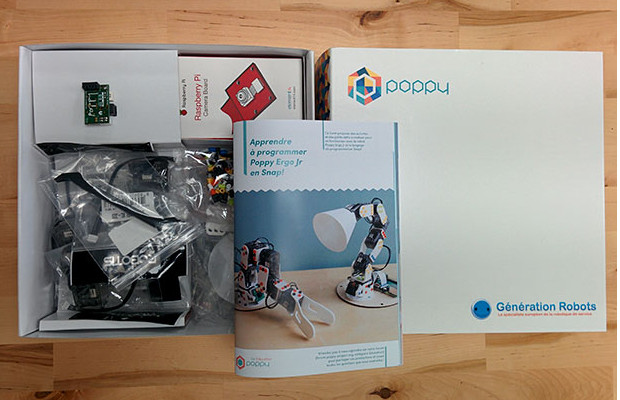
\includegraphics[width=\linewidth]{Figures/Poppy-Box}
        \caption{\label{kit} Robot à construire + un livret pédagogique~\citeB{noirpoudre2016livret}}
    \end{minipage}\hfill
    \begin{minipage}{0.47\linewidth}
        \centering
        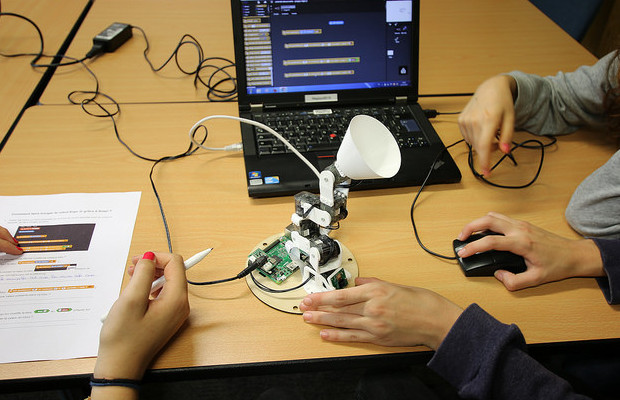
\includegraphics[width=\linewidth]{Figures/Poppy-ergo_at_work}
        \caption{\label{ergo} Robot Poppy~ErgoJr en cours d'utilisation}
    \end{minipage}
    \end{figure}\par%
    Un des objectifs visés par le projet Poppy Éducation était de créer des kits clé en main, facilitant l'auto-formation de l'enseignant et son appropriation du dispositif, avec deux ambitions, que l'enseignant puisse modifier le kit et l’adapter à sa pratique pédagogique et qu’il partage ses réalisations avec la communauté enseignante.
    Il a donc fallu créer des activités dédiées à cette plateforme, former des enseignants, répondre aux problèmes techniques, effectuer un suivi des lycées partenaires, créer des protocoles d'évaluation, \etc. La première étape a été de construire un matériel pédagogique adapté aux concepts abordés en lycée~\citeURL{ICN-prog,ISN-prog}, mais aussi adapté aux utilisateurs et à leur niveau de compétence. La seconde a été principalement de les évaluer en termes de motivation et de satisfaction grâce à des expérimentations à court et long terme faisant varier les conditions.
    Pour évaluer l’impact du kit Poppy~ErgoJr dans le dispositif, nous avons choisi dans un premier temps d'adopter une posture d'observation, afin de recueillir un certain nombre de données qualitatives; nous avons également utilisé des questionnaires standardisés afin d'estimer différentes dimensions.
    Aujourd'hui, plus de 30 lycées sont équipés du kit ErgoJr~\citeA{pdf:etablissements}; et plusieurs expérimentations ont été menées.\par%~\citeT{tab:list_exp}
    Le projet Poppy Éducation est un sous-projet du projet Poppy~\citeURL{poppy-project} qui était initialement soutenu par la Région Nouvelle Aquitaine et l'\bg{UE} au travers du \sbg{FEDER}. Ce projet père œuvrait pour le développement d'une plateforme robotique open-source permettant l'adaptabilité, au sens de la modification rapide de ses composants et de sa structure pour répondre aux besoins expérimentaux en robotique.
    \begin{figure}[!h]
        \centering
        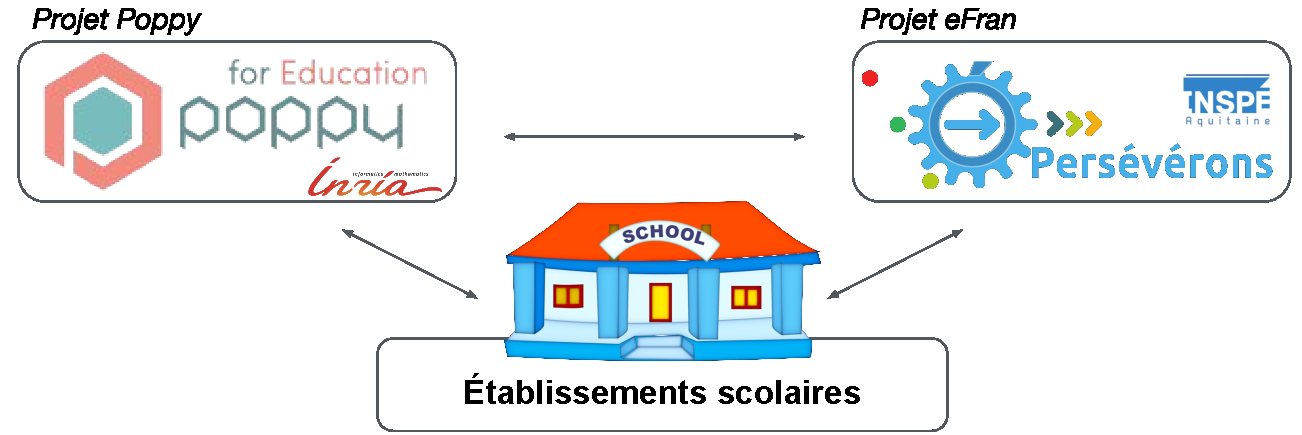
\includegraphics[width=\linewidth]{Figures/Desprez-projet.pdf}
        \caption[Illustration, articulation projet Poppy, eFran et établissements scolaires]{Illustration de l'articulation entre le projet Poppy, le projet eFran et les établissements scolaires.}
        \label{fig:projet}
    \end{figure}\par%
    En parallèle de ce projet, se mettait en place le projet \sbg{perseverons}~\citeURL{perseverons} une réponse à l'\bg{AAP} \sht{eFran}~\citeURL{e-fran}\footnote{\sht{AAP} \sbg{eFran}~\citeURL{e-fran} doté de 30 millions d'\euro{} par la caisse des dépôts via le \sbg{PIA2} et distribué à 22 projets lauréats (1130 k\euro{} pour \sht{perseverons})}. \sht{perseverons} a pour objectif de mesurer l’efficacité réelle des technologies numériques dans l’enseignement pour améliorer la motivation et la persévérance scolaire, et, à long terme, diminuer le décrochage. Le projet propose d’analyser les effets réels de l’usage de deux types d’objets: les robots, les tablettes, en comparant les contextes scolaires et non scolaires des \sht{fablab}. 
    C'est ce projet qui a permis de financer ma thèse, et de pouvoir me permettre de travailler au sein du projet Poppy Éducation à la conception et l'évaluation de kits robotiques open sources issus de la plateforme Poppy.\par%
    Ce type de projet \tiret{open source} a eu un certain nombre de répercussions, et notamment l'émergence d'une communauté~\citeB{ubeda2016logiciels} rassemblant des horizons très divers: bien évidemment la science, communauté à laquelle la plateforme était dédiée; mais aussi les artistes, curieux de découvrir la réalité de la robotique, ou encore l'éducation désireuse de nouvelles ressources afin de répondre aux exigences des nouveaux programmes~\citeURL{planNum}.
    À ce stade, pour la majeure partie des élèves concernés par ces enseignements nouvellement créés (\sht{ISN} et \sht{ICN}), ils n'avaient d'autre connaissance antérieure qu'une expérience autodidacte du numérique et une absence d'expérience en robotique. Ainsi, faute d'une acculturation suffisante, nous constatons qu'il y a une méconnaissance des mécanismes internes à la machine, et donc de leur fonctionnement global et surtout de leurs capacités et limites réelles. La vision dominante est donc largement issue de la culture personnelle de chaque individu, qu'elle soit idyllique, modérée ou apocalyptique, elle est essentiellement véhiculée par la science fiction et n'a que peu d'ancrage dans le réel. Faire évoluer ces représentations pour les faire raccrocher à la réalité est un enjeu de société capital pour aborder le virage technologique du \siecle{21}, et la seule insertion dans ces enseignements spécialisées, bien qu'efficace, n'était pas suffisante.
    \begin{figure}[!h]
    \begin{minipage}{0.6\linewidth}
        \centering
        
\includegraphics[width=0.99\linewidth]{Figures/bot-real.png}
        \subcaption{\label{fig:bot-real} Une vision réaliste}
    \end{minipage}\hfill
    \begin{subfigure}{0.39\linewidth}
        \centering
        
\includegraphics[width=0.975\linewidth]{Figures/bot-magic.png}
        \caption{\label{fig:bot-magic} Une vision idyllique}\vspace{0.15cm}\par%
        
\includegraphics[width=0.975\linewidth]{Figures/bot-fear.png}
        \caption{\label{fig:bot-fear} Une vision apocalyptique}
    \end{subfigure}
    \caption{\label{fig:bot-vision} Différentes visions profanes du numérique et de la robotique}
    \end{figure}{}\par%
    Pour aider chacun à mieux comprendre le monde numérique dans lequel nous vivons et ainsi en faire le meilleur usage possible, l'État Français a choisi d'intégrer en 2017, du cycle 1 au cycle 3, dans tous les programmes scolaires, les sciences du numérique au travers de \cro{Éducation aux médias et à l'information}~\citeURL{EMI}, mais aussi par des actions plus concrètes comme notamment par des exercices en \sht{scra} au Brevet des collèges~\citeURL{brevet}. 
    Cela signifie également, qu'au fur et à mesure il y a un décalage du niveau de compétence attendu.
    Typiquement la suite d'activités pédagogiques IniRobot~\citeB{roy2016inirobot}, exploitant le robot Thymio~\citeB{riedo2013thymio}, a d'abord été conçue pour des élèves de fin de primaire, début collège (12, 13 ans) et aujourd'hui il est majoritairement utilisé chez les 7, 8 ans (début primaire) ou pour des individus totalement novices en robotique (sans limite d'âge).
    Mais il existe de très nombreux dispositifs: nous comptions en 2018~\citeF{fig:list_bot} pas moins de 135 références de robots éducatifs disponibles à la vente sur \noColorHref{www.generationrobots.com}{generationrobots.com}~\citeURL{GR} .
    Dans ce contexte, comment un enseignant peut réaliser un choix éclairé, au regard des besoins de sa classe et de ses propres compétences et envies?
    Dans le but d'offrir aux enseignants une vision objective des potentialités de chaque ressource, il est nécessaire d'évaluer les caractéristiques de ces plateformes ainsi que leur impact sur les apprenants de façon rigoureuse et scientifique.\par%
    Différents éléments sont caractéristiques de la robotique tels que la mobilité ou la forme des robots~\citeB{ben2018elements}, et il en est de même pour les langages de programmation, qu'ils soient visuels ou textuels. Certaines de ces caractéristiques permettent d'exploiter un ou plusieurs leviers pédagogiques par l'enseignant, comme par exemple avec le repositionnement de la place de l'erreur qu'implique le caractère interactif et tangible du robot. C'est notamment ce que soulignait Seymour Papert~\citeB{papert1980mindstorms} lorsqu'il développait sa vision constructiviste de la robotique pédagogique, constructivisme au sens de Piaget~\citeB{ackermann2001piaget}. Cependant, la pédagogie n'est pas intrinsèque à l'outil utilisé mais bien dans son usage lorsqu'il est prescrit par un initié. De plus, cette pédagogique ne peut s'exprimer qu'au travers des différentes contraintes induites par le milieu scolaire, comme exemple, le respect des programmes \tiret{régulièrement réformés~\citeURL{reforme,Frise-educ}}, ou la gestion externalisée du réseau informatique interne à l'établissement (\cf \bg{elib} géré par l'académie).
    Pour aider tout à chacun à mieux envisager les différentes méthodes et principes des pédagogies, il est bon de rappeler quelques notions élémentaires identifiées par les sciences au fil des années. 
    Différentes approches existent, principalement axées autour de la méta-théorie de l'auto-détermination~\citeB{deci1991motivation}, comme le modèle de Viau~\citeB{viau1997vers} ou plus simplement la notion de \sht{flow}~\citeB{nakamura2014concept} ou du besoin d'accomplissement~\citeB{atkinson1957motivational}. D'autres éléments permettent de mieux définir quel procédé préconiser, ou proscrire, dans la conception des activités proposées afin de maximiser leur efficacité. Parmi ces éléments, ceux issus des sciences cognitives nous éclairent sur de nombreux effets \tiret{parfois contre-intuitifs} engendrés par tel ou tel type de tâche \etou contexte, nous pouvons notamment citer la théorie de la charge cognitive~\citeB{sweller1988cognitive} ou encore de nombreux travaux effectués dans le cadre des fonctions exécutives~\citeS{sec:fx-exe} ou le cadre de l'ergonomie des interfaces avec les critères de Scapin~\citeB{scapin1997ergonomic} ou les heuristiques de Nielsen~\citeB{nielsen1994usability}.
    Pour évaluer si ces dispositifs sont fonctionnels et offrent une qualité d'interaction suffisante, plusieurs outils existent, notamment via des questionnaires auto-rapportés comme le \sht{SUS}~\citeB{brooke2013sus} \tiret{pour l'utilisabilité} ou l'\sht{ATT}~\citeB{lallemand2015creation} \tiret{pour l'\sht{UX}}. 
    Mais d'autres éléments sont à évaluer, d'une part, par ce que cela ne garantie rien sur l'acceptation d'une technologie car d'autres facteurs rentrent en jeu comme le montre le modèle TAM~\citeB{davis1989user} et UTAM~\citeB{venkatesh2012consumer}; mais d'autre part, car nous cherchons également à déterminer ici l'impact de ces technologies de façon plus globale. C'est pourquoi, nous avons également évalué la motivation via, entre autres, le \sht{IMI}~\citeB{mcauley1989psychometric} et ses différentes sous-échelles; mais aussi les connaissances via des mini \sht{QCM} ou l'acceptabilité de la robotique en général par le sondage \sht{EURO382}~\citeB{eurobarometer2012382}.
    Ces évaluations ont pris deux axes: \Li un protocole longitudinal écologique et \ii des protocoles ponctuels expérimentaux. 
    \begin{figure}[!h]
    \begin{minipage}{0.63\linewidth}
            \centering
        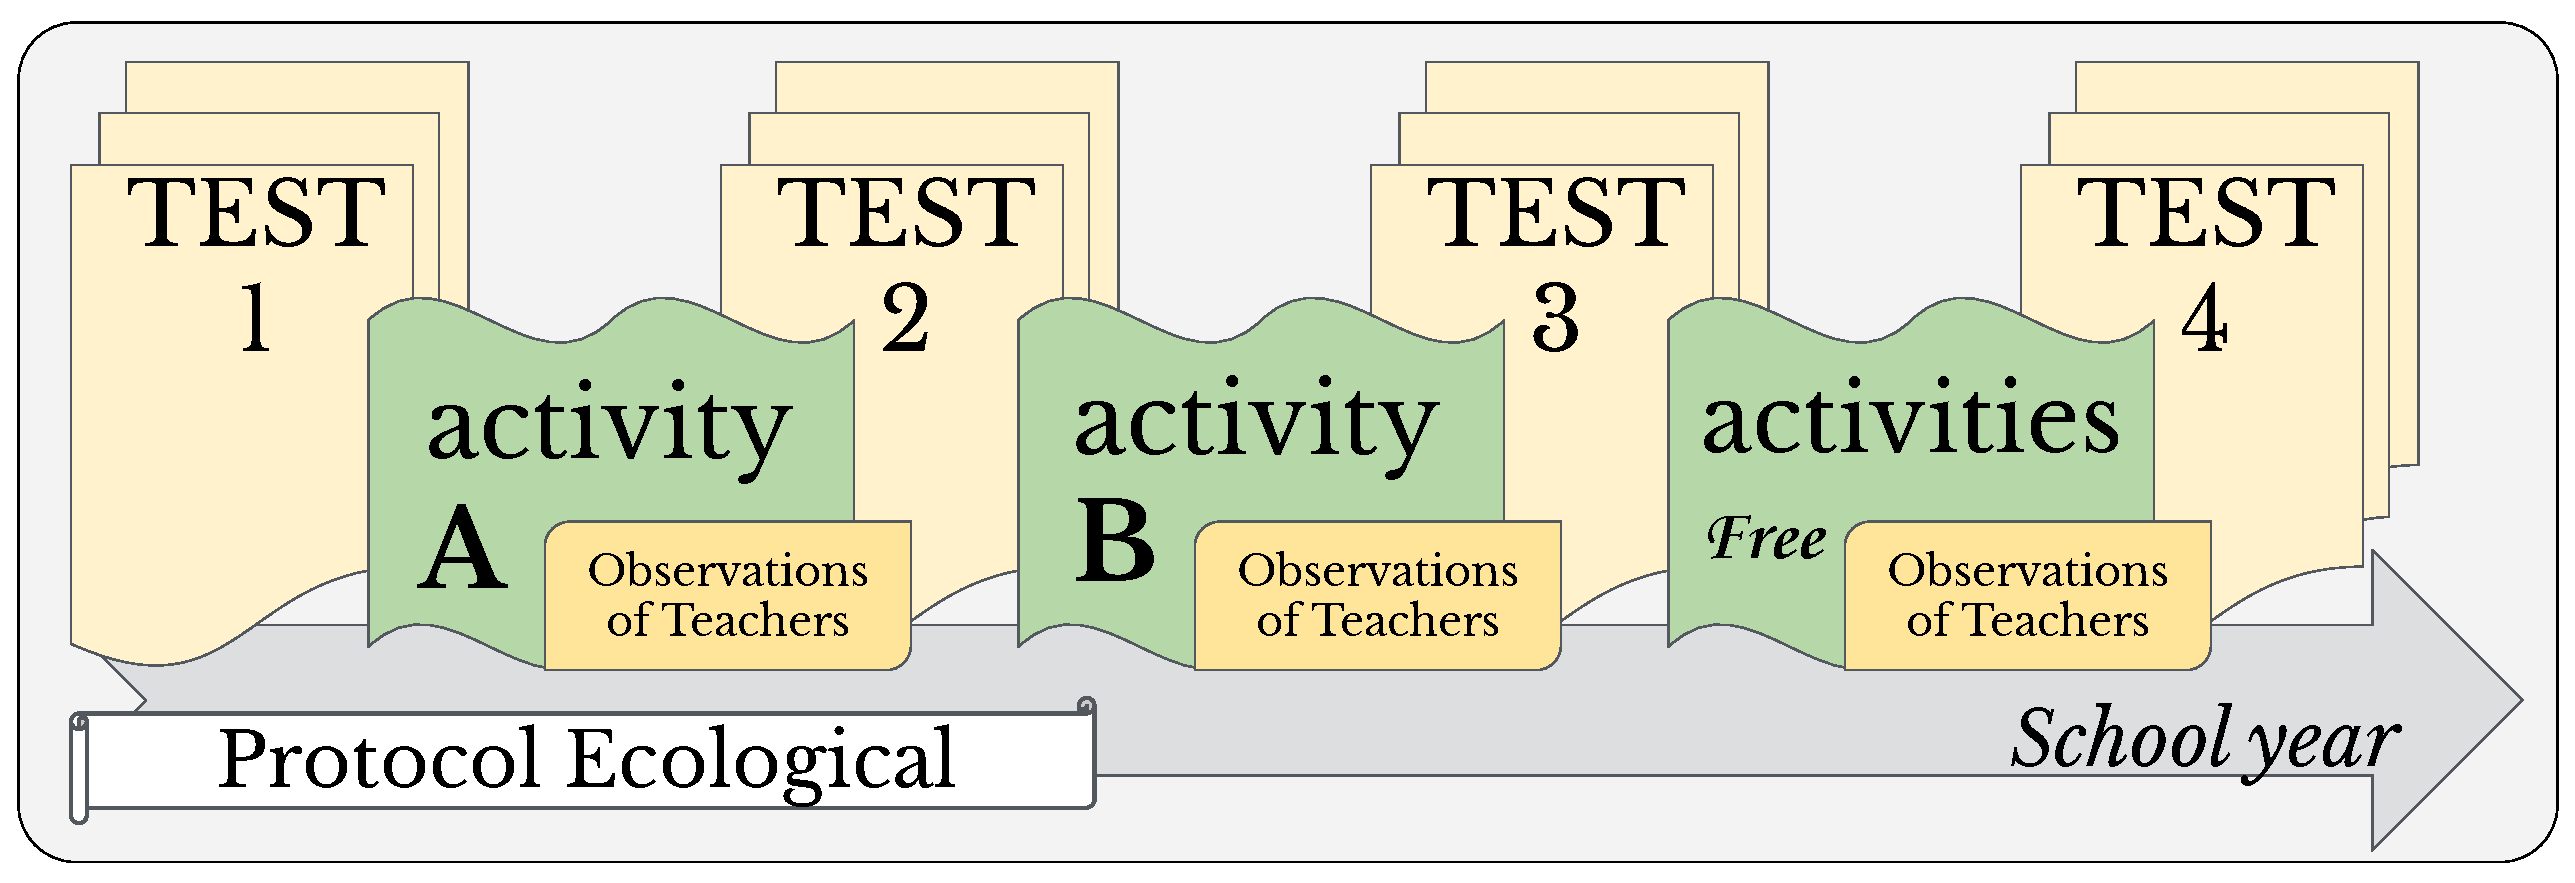
\includegraphics[width=\linewidth]{Figures/Desprez-protocole-eco.pdf}
        \subcaption{Protocole écologique}
        \label{fig:protocole-eco}
    \end{minipage}\hfill    
    \begin{minipage}{0.36\linewidth}
            \centering
        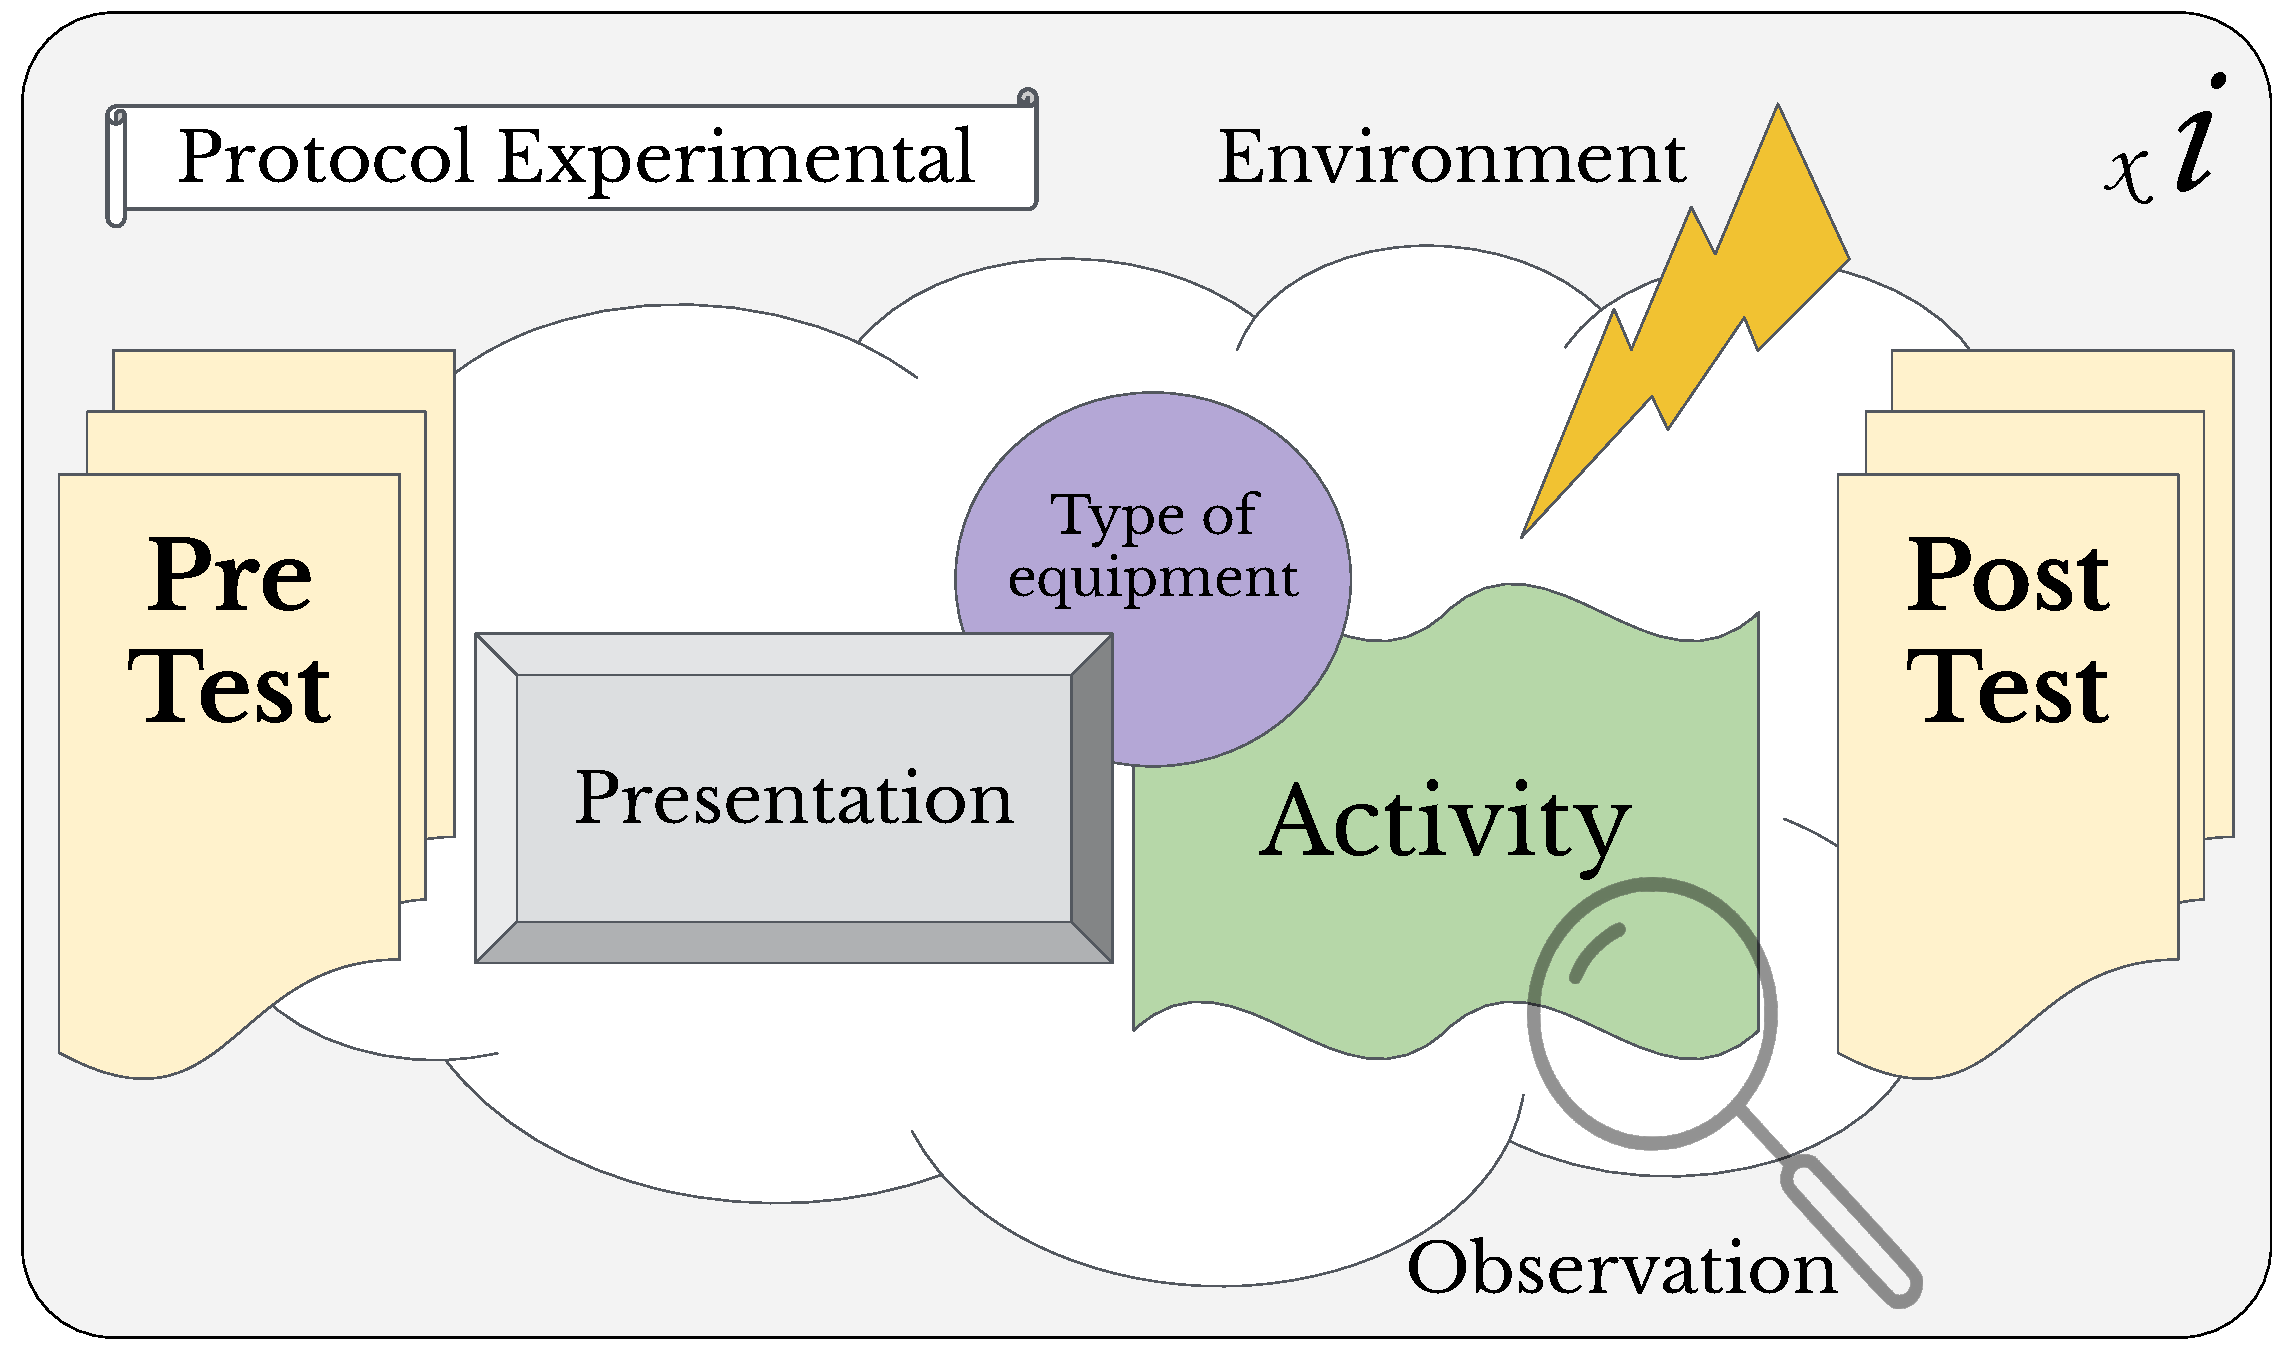
\includegraphics[width=\linewidth]{Figures/Desprez-protocole-exp.pdf}
        \subcaption{Protocole expérimental}
    \label{fig:protocole-exp}
    \end{minipage}
    \caption{Protocole générique, Desprez~\citeB{desprezPoster-efran,desprezPoster-EDMI}}
    \label{fig:protocole}
    \end{figure}\par%
    Nous nous sommes également intéressés, via des protocoles innovants, à des questions plus fondamentales, comme l'impact de donner un nom à son robot~\citeF{fig:proto-name_for_bot}.\par%
\subsection*{Questions de recherche}\myPhantom{subsection}{Questions de recherche}
    La question de recherche générale soulevée dans cette thèse est vaste, et reste un champ grand ouvert de la recherche tant en robotique qu'en éducation:\par%
    \QR{Quels sont les impacts de l'intégration de la robotique pédagogique dans le milieu scolaire; en matière d'acceptabilité de la robotique en général;\break de motivation à réaliser des activités intégrant de telles ressources; et enfin,\break en matière de connaissances acquises}\par%
    Une seconde question est de déterminer quels sont les facteurs incorporés dans ces ressources qui influencent ces impacts. Mais, en préambule, il est intéressant de chercher à déterminer quels sont les éléments permettant une bonne utilisabilité des ressources mais aussi ceux favorisant leur appropriation et \textit{in fine} leur dérivation.
    Il semblerait que ces éléments soient liés. Mais,
    \QR{Existe-il une corrélation entre utilisabilité et appropriation}
    C'est ce que nous essaierons de montrer via, d'une part, des résultats quantitatifs issus des questionnaires \sht{SUS} et \sht{ATT}; et d'autre part, via une étude de cas qualitative sur l'appropriation des enseignants partenaires à notre plateforme.\par%
    Une autre question, souvent établie comme postulat, mais qui reste à démontrer dans notre contexte:
    \QR{Existe-il une corrélation entre connaissances et acceptabilité}
    En effet, la robotique et le numérique étant omniprésents mais invisibles aux non-initiés, en prendre conscience pourrait amener un sentiment de rejet. A contrario, la principale source d'information sur ces domaines étant \tiret{encore jusqu'à il y a peu} la seule science fiction (dépeignant une réalité de la robotique fantasmée \eg AstroBoy, Irobot, Terminator, Minority report,\etc\footnote{Iconographie célèbre: AstroBoy, Osamu Tezuka 1952; Irobot, Isaac Asimov 1967; Terminator, James Cameron 1984; Minority report, Steven Spielberg 2002}), nous pouvons imaginer qu'une augmentation des connaissances favoriserait l'acceptation.
    Cependant, étant difficile d'établir concrètement le niveau initial de connaissances qu'ont les élèves en robotique, nous nous poserons plus simplement, la question suivante:
    \QR{Pratiquer des activités en robotique affecte-t-il notre vision de la robotique}
    Pour déterminer cela, nous avons eu recours au questionnaire \bg{EURO382} sur une population de 276 sujets, et nous constatons, entre autres, que effectivement, pratiquer de telles activités améliore l'acceptation des individus pour la robotique. Mais, y a-t-il des éléments dans ces activités plus déterminants que d'autres? Cette étude ne nous a pas permis de le montrer. En revanche, certains éléments, plus fondamentaux, ont pu être identifiés comme déterminant. En partant de cette question:
    \QR{Donner un nom à un robot permet-il une plus grande proximité avec\break l'utilisateur}
    Nous avons mis au point un protocole permettant de mettre en évidence l'impact de cette dimension \tiret{nommer le robot} sur la peur perçue des sujets pour la robotique, et ceci via une mesure effectuée par le questionnaire \sht{NARS}. Nos résultats montrent que nommer le robot fait croître la peur; cependant, nous montrons également, que ce niveau de peur est maximal en pré-test et donc que, indépendamment de la condition, être mis en présence d'un robot (ici le Poppy humanoïde en vidéo) améliore les résultats au \sht{NARS}.\par%
    Un autre postulat porte sur les questions de motivation et son lien supposé avec l'acquisition de connaissances; mais,
    \QR{Existe-il une corrélation entre motivation et connaissances}
    En effet, certaines recherches s'interrogent sur les leviers motivationnels pour maximiser les apprentissages en évaluant uniquement la motivation et en supposant son impact positif sur l'acquisition de connaissances. Cependant, ce lien est plus complexe et ne relève pas d'une corrélation directe: accroître la motivation améliorera l'engagement et la persévérance dans la réalisation d'activités mais pas leur réussite ni même la rétention des informations s'y trouvant. En revanche, à l'inverse, être amotivé rendra l'engagement plus difficile et le décrochage plus fréquent. 
    La curiosité des individus étant naturellement portée vers la nouveauté; dans notre contexte \tiret{ici les nouvelles technologies, et plus particulièrement la robotique} nous constatons un gain motivationnel. Mais comment un enseignant peut-il le maximiser? Par exemple, 
    \QR{Dans le cadre d'une tâche de construction d'un robot, un enseignant doit-il privilégier une approche modulaire ou une approche linéaire}
    Nous avons montré, qu'une approche modulaire, été plus efficace (\ie construction plus rapide) mais que le sentiment de contrôle perçu par les élèves \tiret{recueilli par le \sht{IMI}} été plus faible dans cette condition alors même qu'ils avaient \tiret{objectivement} plus de contrôle. Ceci montre bien le besoin d'études spécifiques sur des facteurs isolés afin de pouvoir extraire des conclusions fiables. %\par%
    Un autre point que nous avons souhaité soulever porte sur la méthode de formulation. En effet,
    \QR{Est-il préférable d'expliquer à l'élève le principe de la \bg{BSM} de manière théorique ou, au contraire, est-il préférable de laisser l'élève explorer le comportement par pure manipulation} 
    Nos résultats montrent un avantage pour l'exploration en autonomie, non seulement pour la perception de l'effort à fournir afin de résoudre le défi de l'activité (mesuré par le \sht{IMI}), mais aussi sur la compréhension du concept de boucle (mesuré par un \sht{QCM}).\par%
    Pour aller plus loin sur ces notions de tangible, et au vu des contraintes budgétaires, nous nous sommes intéressés à une alternative offerte: les simulateurs. Ainsi,
    \QR{Une version simulée de robot est-elle suffisante à la pratique d'activités robotiques, ou une version réelle est-elle nécessaire}
    Nos premiers résultats montrent un avantage pour la version réelle. Cependant, nos premières conclusions seraient que le besoin de recourir à une version réelle ou simulée dépend plus de l'activité, des objectifs pédagogiques, des notions présentées que de la discipline abordée. D'autres études sont nécessaires afin de compléter ces résultats.
\subsection*{Présentation du plan}\myPhantom{subsection}{Présentation du plan}
    \myPhantom{subsubsection}{Première Partie}
        Ainsi, nous commençons par aborder un état de l'art qui, loin d'être exhaustif, reste volumineux et représente une contribution en soi.
        En effet, les nombreux champs disciplinaires abordés dans cette thèse imposent de définir plusieurs contextes et concepts qui leurs sont associés; et ce, selon différents points de vue.
        Articuler ces différents champs et les rendre cohérents a été un apport indispensable pour la conception et l'évaluation du kit robotique pédagogique ErgoJr en lui-même, mais aussi, sur l'évaluation de son impact.\par%
        \myPhantom{paragraph}{Chapitre 1}
            Ainsi, en tout premier lieu, nous présenterons dans le chapitre~1 les contraintes légales quant à l'utilisation de tels dispositifs et les effets collatéraux de celles-ci.
            Nous développerons ensuite les différentes caractéristiques de la robotique et plus particulièrement nous donnerons plusieurs exemples de robots éducatifs: nous aborderons aussi bien leurs structures, leurs mobilités, leurs formes que leurs modalités d'interaction et les langages de programmation qui leurs sont associés.%\par%
        \myPhantom{paragraph}{Chapitre 2}
            Après ce tour d'horizon des robots existants, nous rentrerons plus au cœur de notre environnement: l'environnement scolaire.
            À ces fins, nous commencerons par préciser dans le chapitre~2 les enjeux de l'intégration des sciences du numérique dans cet écosystème; puis les différentes visions et prescriptions étatiques, notamment au travers de la présentation des programmes \sht{ICN} et \sht{ISN} et des différentes réformes accompagnant ces nouveaux enseignements.
            À cela, nous ajouterons quelques réalités du terrain telles que les contraintes matérielles ou le besoin en formation dans ces domaines.
            Puis, nous enchaînerons sur une notion capitale à la constitution de ressources pour cet environnement: la pédagogie, et les différents courants qui lui sont associés. Enfin nous donnerons quelques exemples issus du passé sur l'introduction de nouvelles technologies dans l'environnement scolaire.%\par%
        \myPhantom{paragraph}{Chapitre 3}
            L'un des objectifs initiaux de ce travail était de créer des ressources ayant un impact quantifiable sur la motivation.
            Un préalable à ceci est donc de définir les notions de motivation et les paradigmes qui permettent son étude. À ces éléments présentés dans le chapitre~3, il a été jugé utile d'y ajouter quelques notions issues de disciplines connexes telles que les sciences cognitives ou les neurosciences pour mieux identifier les déterminants de notre contexte.\par%
        \myPhantom{paragraph}{Chapitre 4}
            Après ce tour d'ensemble des bases théoriques (robotique, pédagogie et motivation) nécessaire à la conception de dispositifs pédagogiques innovant; le rappel des contraintes légales s'y rapportant (programme officiel et licence); et leurs contextes d'intégration (enjeux, utilisateur cible, matériel et formation); il convient de préciser les implications de l'usage d'outils pédagogiques intégrant, d'une part, des outils numériques et, d'autre part, des outils robotiques notamment à travers trois aspects: \Li L'accessibilité de l'information, \ii le rapport à l'erreur et \iii la notion de tangible. C'est ce qui est fait dans le chapitre~4.%\par%
        \myPhantom{paragraph}{Chapitre 5}
            Une fois ces derniers aspects posés, nous aborderons dans le chapitre qui suit les différents concepts, notions et pratiques que nous avons retenus pour l'initiation aux sciences du numérique ainsi que, 
            comment nous les avons définis et exploités.%\par%
        \myPhantom{paragraph}{Chapitre 6}
            Le dernier chapitre de notre état de l'art abordera les aspects spécifiques à l'\sbg{IHM} à travers notamment les implications des effets de double tâche et les principes d'affordance.
            Et, de manière plus générale, nous rappellerons quelques critères d'utilisabilité; et, de manière plus spécifiques, aux kits robotiques, nous aborderons les questions d'appropriation et d'acceptabilité de ces technologies, indispensables à leur intégration sur le long terme.\par%
    \myPhantom{subsubsection}{Deuxième Partie}
        Mais avant de pouvoir évaluer leur intégration et leur impact, il faut concevoir ces outils et c'est l'objet de la seconde partie.
        \myPhantom{paragraph}{Chapitre 1}
            Divisé en quatre chapitres, elle présente dans un premier temps la démarche de co-construction qui a été la nôtre; avec cette particularité que celle-ci fut initiée par les utilisateurs finaux et non par les développeurs.
        \myPhantom{paragraph}{Chapitre 2}
            Nous présenterons donc dans un deuxième chapitre les origines de la plate-forme Poppy et en quoi elle a suscité un intérêt pour ses utilisateurs issus du monde pédagogique.
            Puis, les différents outils permettant d'animer la communauté qui ont été mis en place et adaptés à ce public spécifique.
            
            Dans ce même chapitre seront également présentées les caractéristiques hardware et software du robot ErgoJr; et ce qui a motivé leur choix.
        \myPhantom{paragraph}{Chapitre 3}
            Le troisième chapitre présentera les différentes ressources pédagogiques qui ont été créées pour constituer le kit ErgoJr. Nous les aborderons notamment à travers les modalités pédagogiques qui leur sont associées; ainsi que via
            plusieurs exemples présentant des activités issues de la phase de co-conception, d'autres issues des élèves et d'autres ayant servi de matériel pour les évaluations présentées dans la troisième partie de ce manuscrit.
        \myPhantom{paragraph}{Chapitre 4}
            Mais avant d'aborder cette partie, nous développerons dans le 4\ieme et dernier chapitre (de la partie conception) les autres créatures ayant été générées à partir du kit ErgoJr: PoppyDragster et PoppyDiplo; et, plus généralement, les éléments permettant une dérivation \etou une personnalisation du kit ErgoJr.\par%
    \myPhantom{subsubsection}{Troisième Partie}
        Dériver le kit original pour les besoins d'un projet spécifique est une marque d'appropriation du kit initial.
        Mais d'autres indicateurs nous permettent d'évaluer l'impact de l'intégration de ce kit dans l'environnement scolaire.
        \myPhantom{paragraph}{Chapitre 1}
            Ainsi, dans le premier chapitre de cette troisième partie, nous aborderons les différents outils d'analyse à notre disposition pour évaluer cet impact; notamment nous présenterons les différents questionnaires qui ont été utilisés et les méthodologies d'analyses, que ce soit en termes d'étude de cas, que de constitution de métrique.
            Dans ce même chapitre, nous aborderons également les questions éthiques relatives aux études ayant comme sujet l'humain et les différents protocoles qui ont été mis en place en conséquence.
        \myPhantom{paragraph}{Chapitre 2}
            Dans le deuxième chapitre, nous présenterons les résultats qualitatifs issus de ce travail; notamment à travers une étude de cas sur l'appropriation qu'ont eu 10 enseignants partenaires du projet, mais aussi, au travers des différentes structures ayant soutenu et pérennisant aujourd'hui le projet.
        \myPhantom{paragraph}{Chapitre 3}
            Le troisième chapitre de cette partie sur l'évaluation est divisée en 4~sous-chapitres: \Li l'utilisabilité et l'\sht{UX}, \ii l'acceptabilité de la robotique, \iii la motivation, et \iiii les connaissances.\par%
            \myPhantom{subparagraph}{Sous-Chapitre 1}
                Dans ce premier sous-chapitre, deux expérimentations seront présentées: la première évaluant l'utilisabilité et l'\sht{UX} via respectivement le questionnaire \sht{SUS} et le questionnaire \sht{ATT}, sur une population d'élèves ayant pratiqué des activités avec ErgoJr tout au long de l'année. La seconde exploitant les mêmes questionnaires mais dans le contexte d'une formation au numérique pour des adultes en reconversion professionnelle.
            \myPhantom{subparagraph}{Sous-Chapitre 2}
                Concernant l'acceptabilité, nous avons relevé cette dimension via le questionnaire \sht{EURO382} sur la même population d'élèves ayant complété le \sht{SUS} et l'\sht{ATT} dans le sous-chapitre précédent.
                Ce questionnaire n'étant pas standardisé, une analyse question par question a été nécessaire.
                Et, même si aucune interprétation générale n'a pu être extraite, de nombreux enseignements en ont été tirés.
                Nous avons également abordé cette question d'acceptabilité via une notion plus anodine d'apparence: L'impact de nommer son robot; notamment sur deux dimensions: \Li  La paréidolie\footnote{Ici, au sens de reconnaître des émotions humaines mimées par un robot} et \ii \cro{la peur} envers les robots (mesurée ici via le questionnaire \sht{NARS}).
            \myPhantom{subparagraph}{Sous-Chapitre 3}
                Le troisième sous-chapitre \tiret{dédié à la motivation} commence par représenter une 1\iere expérience n'ayant pas abouti à des passations mais ayant fourni plusieurs ressources qui méritent d'être mentionnées. Il se poursuit en présentant deux expérimentations, l'une portant sur la contrôlabilité dans une activité de construction d'un robot, l'autre sur les modalités de présentation de concepts associés à la robotique (\ie la \bg{BSM}).
            \myPhantom{subparagraph}{Sous-Chapitre 4}
                Le dernier sous-chapitre porte sur la question d'acquisition de connaissances, plus précisément, nous verrons l'impact de la présentation du concept de \bg{BSM} (présenté dans le sous-chapitre précédent) sur  l'appréhension de ce concept à travers la réussite un mini \sht{QCM} en fin d'activité. D'autre part, nous présenterons également dans ce sous-chapitre une expérimentation pilote qui a été menée sur l'impact de l'utilisation d'une version simulée du robot sur la motivation et la compréhension de cette activité; sera également présentée,
             l'expérimentation contrôlée \tiret{mais non réalisée encore} issue de cette expérimentation pilote et portant sur le développement des compétences viso-spatiales.\par%
    \myPhantom{subsubsection}{Les conclusions et résumés}
        Chaque chapitre présent dans ces trois premières parties sont agrémentés d'un résumé en en-tête; et, chacune de ces 3~parties possède une conclusion intermédiaire.
        De plus, les conclusions et discussions de chacune des expérimentations présentées sont intégrées directement avec les présentations de ces expériences.
    \myPhantom{subsubsection}{Discussion}
        Ainsi, nous abordons dans une quatrième partie une courte discussion. Celle-ci, composée de 5~éléments, a pour objet de revenir sur les questions exposées ici dans cette introduction.
        À savoir, l'éventuelle existence d'une corrélation entre utilisabilité et appropriation; entre motivation et acquisition de connaissances; et, entre connaissances et acceptabilité de la robotique. Nous profiterons de cette discussion pour revenir sur quelques éléments issus des phases de conception et d'évaluation.
    \myPhantom{subsubsection}{Conclusion}
        La conclusion générale aura pour objectif de reprendre les différents éléments présentés dans ce manuscrit, pour en extraire les résultats et perspectives les plus pertinents.\par%
\subsection*{Contribution}\myPhantom{subsection}{Contribution}
    \myPhantom{subsubsection}{Juin 2013}
        Ce travail est avant tout un travail d'équipe~\citeT{tab:poppy_team}, personnellement j'ai découvert la plateforme Poppy en 2013 lors d'un travail d'étude et de recherche qui clôturait ma \textsc{Licence} en mathématiques et informatique à l'Université de Bordeaux
    \myPhantom{subsubsection}{Mars à Juillet 2014}
        L'année suivante, lors de mon de \textsc{Master} en sciences cognitives (dans la même université), j'ai réalisé un stage de 4 mois dans le laboratoire \textsc{Flowers} où mon travail a consisté à rédiger \etou traduire de la documentation et des tutoriels destinés à la prise en main du robot humanoïde Poppy.
        Cela venait répondre à la demande naissante des utilisateurs issus du monde pédagogique et artistique souhaitant exploiter cette plate-forme.\par%
    \myPhantom{subsubsection}{Janvier à Juillet 2015}
        En 2015, je réalisais mon second stage dans la même équipe (pour une durée de 6 mois). Entre ces deux stages, l'équipe Poppy projet \tiret{constituée, à l'époque, par Pierre Rouanet, Matthieu Lapeyre et Nicolas Rabault} a entrepris, d'une part, de créer la première ébauche du robot ErgoJr; basée sur le robot Ergo~senior, mais dotée de moteurs moins coûteux; et d'autre part, d'implémenter \tiret{par défaut} une entrée dans l'\sht{api} permettant d'exploiter des \cro{blocs} dans le langage de programmation visuelle \sht{snap}.
        Mon stage (en collaboration avec Marie Demangeat, une autre stagiaire du même \textsc{Master}) consistait alors à constituer du matériel expérimental permettant d'évaluer l'impact de l'utilisation du robot ErgoJr en classe.
        Pour ce stage, nous avons créé un questionnaire accès sur la motivation et sur la compréhension des concepts présentés dans les activités que nous avions développées pour cette occasion:
        de mon côté, l'activité se basait sur une série de vidéos; Marie, elle, développa l'activité danse.
        En parallèle de cela, nous commencions la première analyse des contraintes et besoins des enseignants.
        À ce stade, un ingénieur stagiaire (ENS Électronique et Application, Cergy Pontoise) était également présent Théo Segonds; futur ingénieur de recherche du projet Poppy Éducation. Il avait alors axé son stage sur le développement électronique et software du robot ErgoJr.\par%
        Sur la même période, un ingénieur pédagogique: Stephanie Noirpoudre, a été recrutée pour faire le lien avec les enseignants et entamer la démarche de co-construction des ressources pédagogiques. C'est, entre autres, elle qui s'occupa de mettre en place les différentes réunions, de faire le suivi régulier des enseignants (\eg téléphone, mail, visite, \etc)) et de compiler les ressources qu'ils avaient fournies sous la forme de pages web aujourd'hui disponibles sur le site Poppy éducation. Nous lui devons également l'analyse poussée des programmes \sht{ICN} et \sht{ISN} et la rédaction du livret pédagogique.\par%
    \myPhantom{subsubsection}{Année scolaire 2016-2017}
        Le site Poppy Éducation fut créé courant 2016-17, il reprend les bases techniques du site Poppy project, mais, son architecture a été construite en collaboration avec les enseignants via le travail d'une stagiaire en \textsc{Master}~\sht{UX}~\textit{design}, Innovation et Complexité (Compiègne): Aurélie Lopes.
        Nous pouvons également citer le travail de Kelian Schindowsky en stage de \textsc{Master} \sbg{SIC} qui s'occupa notamment de la mailing-liste et de l'harmonisation des différents supports de communication tel que Twitter.\par%
        En 2016-17, un autre ingénieur a été recruté: Damien Caselli, avec comme spécialité le développement web. Parmi ses réalisations, nous pouvons souligner le \textit{template} de l'interface web aujourd'hui disponible pour les robots Poppy ainsi que le visualisateur exploitant la technologie \textit{WebGL} (directement exécuté dans le navigateur web).\par%
        Pour ma part, dans la continuité des réalisations de mon stage de l'année précédente, mon activité principale a été de construire des ressources pour les élèves et pour les enseignants ainsi que des protocoles permettant de les évaluer selon différents critères.
        Ainsi, j'ai créé plusieurs proto-activités proposées aux enseignants durant la phase de conception; j'ai participé à l'ensemble des réunions de présentation et d'organisation; j'ai également co-animé \tiret{avec Stéphanie et Théo}, les formations données aux enseignants et les ateliers proposés lors de nombreux événements connexes. J'ai également accompagné à plusieurs reprises Stéphanie lors de visites dans les lycées afin d'étudier les réalités du terrain, mais mes principales interactions avec les enseignants s'effectuaient sur le forum Poppy, ou par mail pour l'organisation des passations des différents questionnaires que j'ai sélectionnés notamment en juin 2017 avec le \sht{SUS}, \sht{ATT} et \sht{EURO382}.\par%
    \myPhantom{subsubsection}{Année scolaire 2017-2018}
        Pour l'année scolaire 2017-2018, l'objectif était de réaliser une étude longitudinale et écologique. Pour cela, en amont de la rentrée 2017, j'ai défini un protocole permettant d'évaluer les différentes dimensions étudiées dans ce manuscrit. Ce protocole se devait de respecter les différentes contraintes que les enseignants avaient exprimées.
        De plus, s'attaquant à des notions plus \cro{intimes} pour l'individu et relevant un certain nombre de données dites \cro{personnelles} qui leur était associées, une saisine du comité d'éthique (\cf \sht{COERLE}) a été indispensable, ainsi qu'une déclaration à la \sht{CNIL}.
        Ces différentes procédures ont nécessité la mise en place \Li d'un contrat de collaboration avec les établissements scolaires, contrat, que j'ai co-rédigé avec les services juridiques Inria; et \ii  d'un consentement éclairé à destination de l'ensemble des sujets de l'étude, qui a évolué au cours des navettes avec le \sht{COERLE}.
        Après le suivi de ces procédures et la constitution du matériel expérimental (\eg sélection des questionnaires et rédaction en version papier (latex + \sht{OCR}) et numérique (LimeSurvey); protocole; et activité) j'ai compilé l'ensemble des informations à destination des enseignants pour les passations dans une sous-catégorie du site poppy-education.org.
        Cependant, le protocole qui avait été défini n'a pas pu être mis en place dans les délais impartis et son report à l'année suivante impossible du fait des différentes réformes s'opérant actuellement dans les programmes officiels de l'enseignement des sciences du numérique.\par%
        Mais, dès le début de ma thèse, j'ai souhaité avoir cette double approche: \Li écologique et longitudinale; \ii expérimentale et ponctuelle.
    \myPhantom{subsubsection}{Année scolaire 2018-2019}
        Ces deux approches ayant été validées par le \sht{COERLE} nous avons donc rééquilibré en faveur de l'aspect expérimental, et c'est ce qui fut fait durant l'année scolaire 2018-19. Hormis, le protocole de l'étude pilote présentée en section \ref{Exp:Reel_virtuel-pilote} page~\pageref{Exp:Reel_virtuel-pilote}, l'ensemble des expérimentations (protocole et matériel) présentées sont ici le fruit de mon travail. À noter, que pour l'expérimentation menée avec le PoppyDragster, le développement du robot et la rédaction du contenu ont été effectués par Tallulah Gilliard durant un stage \textsc{Master} \sht{UX}~\textit{Desing} (Stockholm, Suède) que je supervisais durant l'année 2019.
        J'ai également supervisé une groupe de 3 étudiants ingénieurs en 3\ieme année de l'ENSAM sur leur projet d'étude en robotique autonome, ce qui donna naissance à la créature PoppyDiplo.
        En plus des ressources pédagogiques que j'ai développées pour ces expérimentations, j'ai développé d'autres ressources utilitaires, par exemple, une version \textit{v2} des blocs \sht{snap}, des vidéos tutorielles ou encore l'intégration des fonctionnalités développées en parallèle par différents contributeurs \ie interface \textit{v1.2}. Une part de mon travail a également été de répondre aux besoins et difficultés exprimés par les utilisateurs au travers du forum, d'abord en collaboration avec Théo et Stéphanie, puis en collaboration avec un utilisateur identifié comme modérateur du forum.
        Pendant que j'effectuais ces tâches, en plus des activités déjà citées: Damien améliorait la collectivité du dispositif, Théo maintenait et développait la partie software et Stéphanie continuait le développement des ressources pédagogiques, notamment par la réalisation d'un \sht{MOOC}; c'est également elle qui encadra les stages de Aurélie et Kélian, Théo encadra Octave Dellorme (recruté pour développer une carte d'extension qui n'a pas été mentionnée ici); et de nombreux utilisateurs développèrent et testèrent leurs propres ressources: totalement originales ou dérivées de l'existante.\par%
    \myPhantom{subsubsection}{Juillet à novembre 2019}
        En 2019, la rédaction d'un article co-écrit par les membres de l'équipe Poppy Éducation fut amorcé, mais les échéances de chacun (\ie contractuelles) n'ont pas permis d'amener ce travail à terme; cependant, il a constitué une formidable ressource pour la constitution de ce manuscrit, notamment pour la Partie 2 "conception".
        Sans le succès de cette phase de conception, il n'y aurait pu avoir le travail d'évaluation que j'ai mené en suivant. Un objectif secondaire à ce manuscrit est de fournir une ressource pour un public autre que scientifique, notamment un public d'enseignants. À ces fins, j'ai constitué un état de l'art diversifié permettant d'expliciter certaines bases théoriques issues de plusieurs disciplines, pour les adapter à notre contexte: la robotique dans l'environnement scolaire. De plus, certains ressorts pédagogiques des activités ici présentées, dans le cadre des expérimentations pour lesquelles elles ont été constituées, sont également développés afin de mieux les appréhender; notamment dans un objectif de reproduction (par des scientifiques ou des pédagogues). Il est également fait mention de différentes ressources additionnelles venant compléter celles ici présentées.
        Dans ce même objectif, le travail que j'ai effectué pour référencer les ressources présentées et les rapports techniques cités (\eg bulletin officiel, \etc) représente également un apport en soi pour la communauté Poppy et est visible dans la partie Webographe (et cité tout au long du texte).
\myPart{État de l'art}
%PageDeGarde
\phantomsection\pdfbookmark[part]{Conception et \'evaluation de kits robotiques p\'edagogiques.}{title}
\thispagestyle{empty}
\newgeometry{left=2.5cm,right=2.5cm,top=1cm,bottom=1.5cm,includeheadfoot}
\addtolength{\evensidemargin}{-\reliure}
\addtolength{\oddsidemargin}{+\reliure}
%%
\pdfbookmark[paragraph]{Auteur: Thibault DESPREZ}{author}
\pdfbookmark[paragraph]{Directeur: Pierre-Yves OUDEYER}{dir}
\pdfbookmark[paragraph]{Co-encadrant: Didier ROY}{codir}
\pdfbookmark[paragraph]{Laboratoire: FLOWERS Inria-BSO}{lab}
\pdfbookmark[paragraph]{Université: Université de Bordeaux}{univ}
\pdfbookmark[paragraph]{Jury:}{jury}
\pdfbookmark[subparagraph]{Président: Thierry VIÉVILLE}{pre}
\pdfbookmark[subparagraph]{Rapporteur: Margarida ROMERO}{rap1}
\pdfbookmark[subparagraph]{Rapporteur: Florent MASSEGLIA}{rap2}
\pdfbookmark[subparagraph]{Invité: Jerome LAPLACE}{inv}
%%
\vspace{-2cm}\hspace{-0.42cm}\noColorHref{https://www.u-bordeaux.fr/}{
\includegraphics[width=160pt]{Figures/logo-univ.png}}
\hfill
\noColorHref{https://www.inria.fr/}{
\includegraphics[width=140pt]{Figures/logo-inria.png}}
\vspace{0.75cm}

\begin{center}
TH\`{E}SE PR\'{E}SENT\'{E}E

POUR OBTENIR LE GRADE DE

\vspace{0.5cm}
\textbf{{\large DOCTEUR DE}}
\vspace{0.1cm}

\noColorHref{https://www.u-bordeaux.fr/}{\textbf{{\large L'UNIVERSIT\'{E} DE BORDEAUX}}}\\
\vspace{0.62cm}
\noColorHref{https://college-doctoral.u-bordeaux.fr/}{\'{E}COLE DOCTORALE} DE\\
\noColorHref{https://ed-mi.u-bordeaux.fr/}{MATH\'{E}MATIQUES ET INFORMATIQUE}
\vspace{0.25cm}

SP\'{E}CIALIT\'{E} : INFORMATIQUE 
\vspace{0.75cm}

Par : {\large\noColorHref{https://thibaultdesprez.com/}{Thibault DESPREZ}}
\vspace{0.7cm}

\hrule

\vspace{1cm}

\textbf{\large Conception et évaluation de kits robotiques pédagogiques.}
\vspace{0.35cm}

{Études écologiques et expérimentales sur l'impact de l'intégration de la robotique dans\\le milieu scolaire, en matière d'acceptabilité, de motivation et de connaissances.}
\vspace{0.9cm}

\hrule

\vspace{0.62cm}
Sous la direction de : \noColorHref{http://www.pyoudeyer.com/}{Pierre-Yves OUDEYER}\\
\vspace{0.15cm}
Co-encadrée par : \noColorHref{https://dproy.wordpress.com/}{Didier ROY}\\
\vspace{0.42cm}

Soutenue le 05/12/2019
\vspace{0.42cm}

\begin{minipage}{0.942\linewidth}
\vspace{0.35cm}
\hspace{20pt}\textsc{\itshape Membres du Jury :}\vspace{0.42cm}\\
{\setstretch{0,9}
%
\noColorHref{http://www.pyoudeyer.com/}{Pierre-Yves OUDEYER.}
{\quad Directeur de Recherche,
\noColorHref{https://flowers.inria.fr/}{Laboratoire FLOWERS} 
\noColorHref{https://www.inria.fr/}{Inria BSO,}
France.}
\quad \textsc{ Directeur de la Thèse}\vspace{0.2cm}\\
%
\noColorHref{https://dproy.wordpress.com/}{Didier ROY.}
{\quad Ingénieur de Recherche,
\noColorHref{https://flowers.inria.fr/}{Laboratoire FLOWERS} 
\noColorHref{https://www.inria.fr/}{Inria BSO,}
France.}
\break \textsc{ Co-Encadrant de la Thèse}\vspace{0.2cm}\\
%
\noColorHref{https://www-sop.inria.fr/members/Thierry.Vieville/index.fr.html}{Thierry VIÉVILLE.}
{\quad Directeur de Recherche,
\noColorHref{https://learninglab.inria.fr/}{Inria, Learning Lab} \& \noColorHref{https://www.inria.fr/recherches/mediation-scientifique}{Mission de Médiation Scientifique,}
\noColorHref{https://www.inria.fr/centre/sophia}{Inria Sophia Antipolis,}
France.}
\quad \textsc{ Examinateur \& Pr\'{e}sident du Jury}\vspace{0.2cm}\\
%
\noColorHref{https://margaridaromero.wordpress.com/}{Margarida ROMERO.}
{\quad Professeure des Universités,
\noColorHref{http://unice.fr/laboratoires/line}{Laboratoire d’Innovation et Numérique pour l’Éducation (LINE),} \noColorHref{http://univ-cotedazur.fr/fr}{Université Côte d’Azur,}
France.}
\quad \textsc{ Rapporteur}\vspace{0.2cm}\\
%
\noColorHref{http://www.florent-masseglia.info/}{Florent MASSEGLIA.}
{\quad Directeur de Recherche,
\noColorHref{https://team.inria.fr/zenith/}{Laboratoire ZENITH,}
\noColorHref{https://inria.fr/}{Inria,}
\noColorHref{http://www.lirmm.fr/}{LIRMM,}
\noColorHref{http://www.cnrs.fr/fr/page-daccueil}{CNRS,}
\noColorHref{https://www.umontpellier.fr/}{Université de Montpellier,}
France.}
\quad \textsc{ Rapporteur}\vspace{0.2cm}\\
%
\noColorHref{https://www.linkedin.com/in/jeromelaplace/}{Jérôme LAPLACE.}
{\quad Directeur d'entreprise,
\noColorHref{https://www.generationrobots.com/fr/}{Génération Robot,}
\noColorHref{https://grlab-robotics.com/}{GR-Lab}
\& Président du Cluster
\noColorHref{http://www.aquitaine-robotics.com/}{Aquitaine Robotics,}
Bordeaux, France.}
\quad \textsc{Examinateur}
%
}
\end{minipage}
\end{center}

\newpage
\loadgeometry{myDefaultGeo}
\ifx\BackGroundColor\undefined
  \nopagecolor
\else
  \pagecolor{\BackGroundColor}
\fi
\pagestyle{plain}
\toPrint

%Resume
\phantomsection\pdfbookmark[part]{R{\'e}sumer}{abstract}
%4000 craractere max
\newcommand\motscle{Kit robotique, Plateforme Robotique Poppy, Robot ErgoJr, Conception, Évaluation}
\newcommand\resume{
Le potentiel des activités pédagogiques robotiques, et en particulier le rôle de l’instanciation physique de ces activités, dans lesquelles la manipulation d’objets numériques est centrale, reste encore à confirmer scientifiquement; en particulier en matière d'utilisabilité réelle en classe et de leur impact sur l’efficacité des apprentissages et sur l’engagement motivationnel des élèves.
Par ailleurs, il semble que ces impacts dépendent aussi de la manière dont ces outils pédagogiques sont utilisés (et détournés) par l'enseignant en classe, ainsi que par le contexte scolaire lui-même.%
Pour ces raisons, ce manuscrit propose dans un premier temps d'articuler un état de l'art issu de champs disciplinaires variés, notamment scientifiques, comme l'informatique et la robotique, l'IHM, la psychologie, les sciences cognitives, ou encore les sciences de l'éducation; mais aussi, d'introduire des éléments d'éthique et des enjeux sociétaux. Cette partie propose également de définir notre milieu: les acteurs (utilisateurs cibles: enseignants et élèves), les prescriptions (objectifs et besoins des programmes officiels), les réalités du terrain (les contraintes: budget, matériel, réforme, formation, \etc). 
Dans un deuxième temps, nous présentons les éléments (hardware, software et ressources) constituant le kit robotique pédagogique Poppy ErgoJr; co-créé et testé par des enseignants issus principalement des sections ICN (seconde) et ISN (terminale) d'Aquitaine et, les membres du projet Poppy Éducation (Inria-BSO). Leur processus de création sera également présenté, tout comme les activités créées pour les besoins des expérimentations présentées dans la partie suivante.
Mais avant celle-ci, nous montrerons 2~exemples de dérivations du kit: PoppyDiplo et PoppyDragster, dont le 2\nd aboutit à une expérimentation portant sur l'impact des ressources documentaires sur le sentiment de contrôle de l'élève (relevé par le IMI) lors d'une tâche de construction collaborative d'un robot. Une 2\nde expérience, avec ErgoJr, portant sur le formalisme des ressources fournies et leur impact motivationnel sera présentée. 
Trois autres thématiques seront abordées: l'utilisabilité mesurée dans un cadre longitudinal et écologique (via le SUS et l'AttrakDiff); l'acceptabilité mesurée via l'Euro382, et un questionnaire innovant, étudiant l'impact de la nomination d'un objet sur la perception de celle-ci; et, l'acquisition de connaissances (via des qcm).
Une étude qualitative est également proposée dans cette partie, entre autres, au travers d'une étude de cas portant sur l'appropriation du dispositif par 10 enseignants.
Nous finirons par une discussion ayant pour objet les questions soulevées en introduction, et ouvrant sur la conclusion générale de ce manuscrit qui rappellera les principaux enseignements de ce travail et ses perspectives d'avenir.
}
\newcommand\keysword{Robotics Kit, Poppy Robotics Platforme, ErgoJr Robot, Conception, Evaluation}
\newcommand\abst{
The potential of robotic educational activities, and in particular the role of the physical instantiation of these activities, in which the manipulation of digital objects is central, remains to be confirmed scientifically; especially in terms of real classroom usability and their impact on the effectiveness of learning and the motivational engagement of students. Moreover, it seems that these impacts also depend on the way in which these pedagogical tools are used (and diverted) by the teacher in class, as well as by the school context itself. For these reasons, this manuscript proposes in a first step in articulating a state of art from a variety of disciplinary fields, notably scientific, such as computer science and robotics, IHM, psychology, cognitive sciences, or the sciences of education ; but also to introduce elements of ethics and societal issues. This part also proposes to define our environment: the actors (target users: teachers and pupils), the prescriptions (objectives and needs of the official programs), the realities of the field (the constraints: budget, material, reform, training, \etc). In a second step, we will present the elements (hardware, software and resources) constituting the educational robotics kit Poppy ErgoJr; co-created and tested by teachers mainly from high school sections of Aquitaine and the members of the Poppy Education project (Inria-BSO). Their creation process will also be presented, as will the activities created for the purposes of the experiments presented in the following section. But before this one, we will show two examples of derivations of the kit: PoppyDiplo and PoppyDragster, whose second ended with an experimentation on the impact of the documentary resources on the feeling of control of the pupil (measured by the IMI) during a task of collaborative construction of a robot. A second experience, with ErgoJr, on the formalization of the resources provided and their motivational impact will be presented. Three other themes will be tackled: usability measured in a longitudinal and ecological framework (via the SUS and AttrakDiff); acceptability measured via Euro382, and an innovative questionnaire, studying the impact of the appointment of an object on the perception of this one; and the acquisition of knowledge (via qcm). A qualitative study is also proposed in this part, among others, through a case study on the appropriation of device by 10 teachers. We will end with a discussion of the questions raised in the introduction, and opening on the general conclusion of this manuscript which will recall the main lessons of this work and its future prospects.
}
%1000 caractere max
\newcommand\vulga{
L'enseignement des sciences du numérique est un enjeu crucial; il sera déterminant sur les usages et choix de société qui seront effectués dans ce domaine. Cet enseignement se fait aujourd'hui, entre autres, à l'école. Et, les dispositifs pour ces apprentissages pullulent, sans pour autant avoir fait l'objet d'étude sur leurs usages et intérêts réels en classe. Cet ouvrage a pour objet de rassembler différents éléments théoriques et pratiques à prendre en considération pour appréhender l'impact de l'introduction de la robotique pédagogique dans l'environnement scolaire. Un second objectif est d'offrir aux enseignants, des clés de lecture pour évaluer la pertinence des objets, dits pédagogiques, qui leur sont proposés; et pour mieux estimer les moyens à leur disposition pour se les approprier. Une des conclusions de ce travail est que l'enseignant est le déterminant principal pour la bonne intégration de ces dispositifs et que cela passe par une bonne appropriation de ces technologies.
}
\newcommand\pop{
The teaching of digital sciences is a crucial issue; it will be decisive on the uses and society's choices that will be made in this field. This teaching is done today, among others, at school. And, the devices for these learnings abound, without having been the subject of study on their uses and real interests in class. The purpose of this book is to bring together different theoretical and practical elements to consider in order to understand the impact of the introduction of educational robotics in the school environment. A second objective is to provide teachers with reading keys to evaluate the relevance of the so-called educational objects offered to them; and to better estimate the means at their disposal to appropriate them. One of the conclusions of this work is that the teacher is the main determinant for the proper integration of these devices and that it requires a good appropriation of these technologies.
}
%%%%%%%%%%%%%%%%%%%%%%%%%%%%%%%%%%%%%%%%%%%%%%%%%%%%%%%%%%%%%%%% display

\phantomsection\pdfbookmark[section]{R{\'e}sumer}{resumFR}
\begin{center}
{\textbf{\Large Conception et évaluation\\\vspace{0.1cm}de kits robotiques pédagogiques.}}\\\vspace{0.5cm}    
\end{center}

\textbf{\centering\large\underline{R\'esum\'e}~:} \\\vspace{0.25cm}

{\myDefautStyle\resume}\\
\vspace{0.5cm}\\
{\textbf{\underline{Mots cl\'{e}s}~:\\\vspace{0.1cm}\motscle}}\\
\phantomsection\pdfbookmark[paragraph]{Mots cl\'{e}s:}{motscle}
\phantomsection\pdfbookmark[subparagraph]{Kits Robotiques}{cle1}
\phantomsection\pdfbookmark[subparagraph]{Platforme Robotique Poppy}{cle2}
\phantomsection\pdfbookmark[subparagraph]{ErgoJr Robot}{cle3}
\phantomsection\pdfbookmark[subparagraph]{Conception}{cle4}
\phantomsection\pdfbookmark[subparagraph]{{\'E}valuation}{cle5}
\toPrint

\phantomsection\pdfbookmark[section]{Abstract}{resumEn}
\begin{center}
{\Large\textbf{Design and evaluation\\\vspace{0.1cm}of educational robotic kits.}}\\\vspace{0.5cm}    
\end{center}

\textbf{\large\underline{Abstract}~:}\\\vspace{0.25cm}

{\myDefautStyle\abst}\\
\vspace{0.5cm}\\
{\textbf{\underline{Keywords}~:\\\vspace{0.1cm}\keysword}}\\
\phantomsection\pdfbookmark[paragraph]{Keywords:}{keywords}
\phantomsection\pdfbookmark[subparagraph]{Robotics Kit}{key1}
\phantomsection\pdfbookmark[subparagraph]{Poppy Robotics Platforme}{key2}
\phantomsection\pdfbookmark[subparagraph]{ErgoJr Robot}{key3}
\phantomsection\pdfbookmark[subparagraph]{Conception}{key4}
\phantomsection\pdfbookmark[subparagraph]{Evaluation}{key5}
\toPrint

\phantomsection\pdfbookmark[section]{R{\'e}sumer vulgaris{\'e}}{resumVulga}
\vspace{3cm}\strut\\
\begin{center}

{\textbf{\Large Résumé de thèse vulgarisé}}\\\vspace{0.45cm}    

\begin{minipage}{0.85\linewidth}
{\myDefautStyle\vulga}
\end{minipage}\vspace{1cm}\\

{\textbf{\Large Thesis Summary popularized}}\\\vspace{0.35cm}    

\begin{minipage}{0.85\linewidth}
{\myDefautStyle\pop}
\end{minipage}\vspace{1cm}\\
\end{center}
\clearpage
\toPrint

%Preface
\fancyhead[L]{}
\phantomsection\pdfbookmark[part]{Pr\'eface}{pre}
%PageDeGarde
\phantomsection\pdfbookmark[part]{Conception et \'evaluation de kits robotiques p\'edagogiques.}{title}
\thispagestyle{empty}
\newgeometry{left=2.5cm,right=2.5cm,top=1cm,bottom=1.5cm,includeheadfoot}
\addtolength{\evensidemargin}{-\reliure}
\addtolength{\oddsidemargin}{+\reliure}
%%
\pdfbookmark[paragraph]{Auteur: Thibault DESPREZ}{author}
\pdfbookmark[paragraph]{Directeur: Pierre-Yves OUDEYER}{dir}
\pdfbookmark[paragraph]{Co-encadrant: Didier ROY}{codir}
\pdfbookmark[paragraph]{Laboratoire: FLOWERS Inria-BSO}{lab}
\pdfbookmark[paragraph]{Université: Université de Bordeaux}{univ}
\pdfbookmark[paragraph]{Jury:}{jury}
\pdfbookmark[subparagraph]{Président: Thierry VIÉVILLE}{pre}
\pdfbookmark[subparagraph]{Rapporteur: Margarida ROMERO}{rap1}
\pdfbookmark[subparagraph]{Rapporteur: Florent MASSEGLIA}{rap2}
\pdfbookmark[subparagraph]{Invité: Jerome LAPLACE}{inv}
%%
\vspace{-2cm}\hspace{-0.42cm}\noColorHref{https://www.u-bordeaux.fr/}{
\includegraphics[width=160pt]{Figures/logo-univ.png}}
\hfill
\noColorHref{https://www.inria.fr/}{
\includegraphics[width=140pt]{Figures/logo-inria.png}}
\vspace{0.75cm}

\begin{center}
TH\`{E}SE PR\'{E}SENT\'{E}E

POUR OBTENIR LE GRADE DE

\vspace{0.5cm}
\textbf{{\large DOCTEUR DE}}
\vspace{0.1cm}

\noColorHref{https://www.u-bordeaux.fr/}{\textbf{{\large L'UNIVERSIT\'{E} DE BORDEAUX}}}\\
\vspace{0.62cm}
\noColorHref{https://college-doctoral.u-bordeaux.fr/}{\'{E}COLE DOCTORALE} DE\\
\noColorHref{https://ed-mi.u-bordeaux.fr/}{MATH\'{E}MATIQUES ET INFORMATIQUE}
\vspace{0.25cm}

SP\'{E}CIALIT\'{E} : INFORMATIQUE 
\vspace{0.75cm}

Par : {\large\noColorHref{https://thibaultdesprez.com/}{Thibault DESPREZ}}
\vspace{0.7cm}

\hrule

\vspace{1cm}

\textbf{\large Conception et évaluation de kits robotiques pédagogiques.}
\vspace{0.35cm}

{Études écologiques et expérimentales sur l'impact de l'intégration de la robotique dans\\le milieu scolaire, en matière d'acceptabilité, de motivation et de connaissances.}
\vspace{0.9cm}

\hrule

\vspace{0.62cm}
Sous la direction de : \noColorHref{http://www.pyoudeyer.com/}{Pierre-Yves OUDEYER}\\
\vspace{0.15cm}
Co-encadrée par : \noColorHref{https://dproy.wordpress.com/}{Didier ROY}\\
\vspace{0.42cm}

Soutenue le 05/12/2019
\vspace{0.42cm}

\begin{minipage}{0.942\linewidth}
\vspace{0.35cm}
\hspace{20pt}\textsc{\itshape Membres du Jury :}\vspace{0.42cm}\\
{\setstretch{0,9}
%
\noColorHref{http://www.pyoudeyer.com/}{Pierre-Yves OUDEYER.}
{\quad Directeur de Recherche,
\noColorHref{https://flowers.inria.fr/}{Laboratoire FLOWERS} 
\noColorHref{https://www.inria.fr/}{Inria BSO,}
France.}
\quad \textsc{ Directeur de la Thèse}\vspace{0.2cm}\\
%
\noColorHref{https://dproy.wordpress.com/}{Didier ROY.}
{\quad Ingénieur de Recherche,
\noColorHref{https://flowers.inria.fr/}{Laboratoire FLOWERS} 
\noColorHref{https://www.inria.fr/}{Inria BSO,}
France.}
\break \textsc{ Co-Encadrant de la Thèse}\vspace{0.2cm}\\
%
\noColorHref{https://www-sop.inria.fr/members/Thierry.Vieville/index.fr.html}{Thierry VIÉVILLE.}
{\quad Directeur de Recherche,
\noColorHref{https://learninglab.inria.fr/}{Inria, Learning Lab} \& \noColorHref{https://www.inria.fr/recherches/mediation-scientifique}{Mission de Médiation Scientifique,}
\noColorHref{https://www.inria.fr/centre/sophia}{Inria Sophia Antipolis,}
France.}
\quad \textsc{ Examinateur \& Pr\'{e}sident du Jury}\vspace{0.2cm}\\
%
\noColorHref{https://margaridaromero.wordpress.com/}{Margarida ROMERO.}
{\quad Professeure des Universités,
\noColorHref{http://unice.fr/laboratoires/line}{Laboratoire d’Innovation et Numérique pour l’Éducation (LINE),} \noColorHref{http://univ-cotedazur.fr/fr}{Université Côte d’Azur,}
France.}
\quad \textsc{ Rapporteur}\vspace{0.2cm}\\
%
\noColorHref{http://www.florent-masseglia.info/}{Florent MASSEGLIA.}
{\quad Directeur de Recherche,
\noColorHref{https://team.inria.fr/zenith/}{Laboratoire ZENITH,}
\noColorHref{https://inria.fr/}{Inria,}
\noColorHref{http://www.lirmm.fr/}{LIRMM,}
\noColorHref{http://www.cnrs.fr/fr/page-daccueil}{CNRS,}
\noColorHref{https://www.umontpellier.fr/}{Université de Montpellier,}
France.}
\quad \textsc{ Rapporteur}\vspace{0.2cm}\\
%
\noColorHref{https://www.linkedin.com/in/jeromelaplace/}{Jérôme LAPLACE.}
{\quad Directeur d'entreprise,
\noColorHref{https://www.generationrobots.com/fr/}{Génération Robot,}
\noColorHref{https://grlab-robotics.com/}{GR-Lab}
\& Président du Cluster
\noColorHref{http://www.aquitaine-robotics.com/}{Aquitaine Robotics,}
Bordeaux, France.}
\quad \textsc{Examinateur}
%
}
\end{minipage}
\end{center}

\newpage
\loadgeometry{myDefaultGeo}
\ifx\BackGroundColor\undefined
  \nopagecolor
\else
  \pagecolor{\BackGroundColor}
\fi
\pagestyle{plain}
\toPrint

%Resume
\phantomsection\pdfbookmark[part]{R{\'e}sumer}{abstract}
%4000 craractere max
\newcommand\motscle{Kit robotique, Plateforme Robotique Poppy, Robot ErgoJr, Conception, Évaluation}
\newcommand\resume{
Le potentiel des activités pédagogiques robotiques, et en particulier le rôle de l’instanciation physique de ces activités, dans lesquelles la manipulation d’objets numériques est centrale, reste encore à confirmer scientifiquement; en particulier en matière d'utilisabilité réelle en classe et de leur impact sur l’efficacité des apprentissages et sur l’engagement motivationnel des élèves.
Par ailleurs, il semble que ces impacts dépendent aussi de la manière dont ces outils pédagogiques sont utilisés (et détournés) par l'enseignant en classe, ainsi que par le contexte scolaire lui-même.%
Pour ces raisons, ce manuscrit propose dans un premier temps d'articuler un état de l'art issu de champs disciplinaires variés, notamment scientifiques, comme l'informatique et la robotique, l'IHM, la psychologie, les sciences cognitives, ou encore les sciences de l'éducation; mais aussi, d'introduire des éléments d'éthique et des enjeux sociétaux. Cette partie propose également de définir notre milieu: les acteurs (utilisateurs cibles: enseignants et élèves), les prescriptions (objectifs et besoins des programmes officiels), les réalités du terrain (les contraintes: budget, matériel, réforme, formation, \etc). 
Dans un deuxième temps, nous présentons les éléments (hardware, software et ressources) constituant le kit robotique pédagogique Poppy ErgoJr; co-créé et testé par des enseignants issus principalement des sections ICN (seconde) et ISN (terminale) d'Aquitaine et, les membres du projet Poppy Éducation (Inria-BSO). Leur processus de création sera également présenté, tout comme les activités créées pour les besoins des expérimentations présentées dans la partie suivante.
Mais avant celle-ci, nous montrerons 2~exemples de dérivations du kit: PoppyDiplo et PoppyDragster, dont le 2\nd aboutit à une expérimentation portant sur l'impact des ressources documentaires sur le sentiment de contrôle de l'élève (relevé par le IMI) lors d'une tâche de construction collaborative d'un robot. Une 2\nde expérience, avec ErgoJr, portant sur le formalisme des ressources fournies et leur impact motivationnel sera présentée. 
Trois autres thématiques seront abordées: l'utilisabilité mesurée dans un cadre longitudinal et écologique (via le SUS et l'AttrakDiff); l'acceptabilité mesurée via l'Euro382, et un questionnaire innovant, étudiant l'impact de la nomination d'un objet sur la perception de celle-ci; et, l'acquisition de connaissances (via des qcm).
Une étude qualitative est également proposée dans cette partie, entre autres, au travers d'une étude de cas portant sur l'appropriation du dispositif par 10 enseignants.
Nous finirons par une discussion ayant pour objet les questions soulevées en introduction, et ouvrant sur la conclusion générale de ce manuscrit qui rappellera les principaux enseignements de ce travail et ses perspectives d'avenir.
}
\newcommand\keysword{Robotics Kit, Poppy Robotics Platforme, ErgoJr Robot, Conception, Evaluation}
\newcommand\abst{
The potential of robotic educational activities, and in particular the role of the physical instantiation of these activities, in which the manipulation of digital objects is central, remains to be confirmed scientifically; especially in terms of real classroom usability and their impact on the effectiveness of learning and the motivational engagement of students. Moreover, it seems that these impacts also depend on the way in which these pedagogical tools are used (and diverted) by the teacher in class, as well as by the school context itself. For these reasons, this manuscript proposes in a first step in articulating a state of art from a variety of disciplinary fields, notably scientific, such as computer science and robotics, IHM, psychology, cognitive sciences, or the sciences of education ; but also to introduce elements of ethics and societal issues. This part also proposes to define our environment: the actors (target users: teachers and pupils), the prescriptions (objectives and needs of the official programs), the realities of the field (the constraints: budget, material, reform, training, \etc). In a second step, we will present the elements (hardware, software and resources) constituting the educational robotics kit Poppy ErgoJr; co-created and tested by teachers mainly from high school sections of Aquitaine and the members of the Poppy Education project (Inria-BSO). Their creation process will also be presented, as will the activities created for the purposes of the experiments presented in the following section. But before this one, we will show two examples of derivations of the kit: PoppyDiplo and PoppyDragster, whose second ended with an experimentation on the impact of the documentary resources on the feeling of control of the pupil (measured by the IMI) during a task of collaborative construction of a robot. A second experience, with ErgoJr, on the formalization of the resources provided and their motivational impact will be presented. Three other themes will be tackled: usability measured in a longitudinal and ecological framework (via the SUS and AttrakDiff); acceptability measured via Euro382, and an innovative questionnaire, studying the impact of the appointment of an object on the perception of this one; and the acquisition of knowledge (via qcm). A qualitative study is also proposed in this part, among others, through a case study on the appropriation of device by 10 teachers. We will end with a discussion of the questions raised in the introduction, and opening on the general conclusion of this manuscript which will recall the main lessons of this work and its future prospects.
}
%1000 caractere max
\newcommand\vulga{
L'enseignement des sciences du numérique est un enjeu crucial; il sera déterminant sur les usages et choix de société qui seront effectués dans ce domaine. Cet enseignement se fait aujourd'hui, entre autres, à l'école. Et, les dispositifs pour ces apprentissages pullulent, sans pour autant avoir fait l'objet d'étude sur leurs usages et intérêts réels en classe. Cet ouvrage a pour objet de rassembler différents éléments théoriques et pratiques à prendre en considération pour appréhender l'impact de l'introduction de la robotique pédagogique dans l'environnement scolaire. Un second objectif est d'offrir aux enseignants, des clés de lecture pour évaluer la pertinence des objets, dits pédagogiques, qui leur sont proposés; et pour mieux estimer les moyens à leur disposition pour se les approprier. Une des conclusions de ce travail est que l'enseignant est le déterminant principal pour la bonne intégration de ces dispositifs et que cela passe par une bonne appropriation de ces technologies.
}
\newcommand\pop{
The teaching of digital sciences is a crucial issue; it will be decisive on the uses and society's choices that will be made in this field. This teaching is done today, among others, at school. And, the devices for these learnings abound, without having been the subject of study on their uses and real interests in class. The purpose of this book is to bring together different theoretical and practical elements to consider in order to understand the impact of the introduction of educational robotics in the school environment. A second objective is to provide teachers with reading keys to evaluate the relevance of the so-called educational objects offered to them; and to better estimate the means at their disposal to appropriate them. One of the conclusions of this work is that the teacher is the main determinant for the proper integration of these devices and that it requires a good appropriation of these technologies.
}
%%%%%%%%%%%%%%%%%%%%%%%%%%%%%%%%%%%%%%%%%%%%%%%%%%%%%%%%%%%%%%%% display

\phantomsection\pdfbookmark[section]{R{\'e}sumer}{resumFR}
\begin{center}
{\textbf{\Large Conception et évaluation\\\vspace{0.1cm}de kits robotiques pédagogiques.}}\\\vspace{0.5cm}    
\end{center}

\textbf{\centering\large\underline{R\'esum\'e}~:} \\\vspace{0.25cm}

{\myDefautStyle\resume}\\
\vspace{0.5cm}\\
{\textbf{\underline{Mots cl\'{e}s}~:\\\vspace{0.1cm}\motscle}}\\
\phantomsection\pdfbookmark[paragraph]{Mots cl\'{e}s:}{motscle}
\phantomsection\pdfbookmark[subparagraph]{Kits Robotiques}{cle1}
\phantomsection\pdfbookmark[subparagraph]{Platforme Robotique Poppy}{cle2}
\phantomsection\pdfbookmark[subparagraph]{ErgoJr Robot}{cle3}
\phantomsection\pdfbookmark[subparagraph]{Conception}{cle4}
\phantomsection\pdfbookmark[subparagraph]{{\'E}valuation}{cle5}
\toPrint

\phantomsection\pdfbookmark[section]{Abstract}{resumEn}
\begin{center}
{\Large\textbf{Design and evaluation\\\vspace{0.1cm}of educational robotic kits.}}\\\vspace{0.5cm}    
\end{center}

\textbf{\large\underline{Abstract}~:}\\\vspace{0.25cm}

{\myDefautStyle\abst}\\
\vspace{0.5cm}\\
{\textbf{\underline{Keywords}~:\\\vspace{0.1cm}\keysword}}\\
\phantomsection\pdfbookmark[paragraph]{Keywords:}{keywords}
\phantomsection\pdfbookmark[subparagraph]{Robotics Kit}{key1}
\phantomsection\pdfbookmark[subparagraph]{Poppy Robotics Platforme}{key2}
\phantomsection\pdfbookmark[subparagraph]{ErgoJr Robot}{key3}
\phantomsection\pdfbookmark[subparagraph]{Conception}{key4}
\phantomsection\pdfbookmark[subparagraph]{Evaluation}{key5}
\toPrint

\phantomsection\pdfbookmark[section]{R{\'e}sumer vulgaris{\'e}}{resumVulga}
\vspace{3cm}\strut\\
\begin{center}

{\textbf{\Large Résumé de thèse vulgarisé}}\\\vspace{0.45cm}    

\begin{minipage}{0.85\linewidth}
{\myDefautStyle\vulga}
\end{minipage}\vspace{1cm}\\

{\textbf{\Large Thesis Summary popularized}}\\\vspace{0.35cm}    

\begin{minipage}{0.85\linewidth}
{\myDefautStyle\pop}
\end{minipage}\vspace{1cm}\\
\end{center}
\clearpage
\toPrint

%Preface
\fancyhead[L]{}
\phantomsection\pdfbookmark[part]{Pr\'eface}{pre}
%PageDeGarde
\phantomsection\pdfbookmark[part]{Conception et \'evaluation de kits robotiques p\'edagogiques.}{title}
\input{Texte/Partie0/PageDeGarde.tex}
\newpage
\loadgeometry{myDefaultGeo}
\ifx\BackGroundColor\undefined
  \nopagecolor
\else
  \pagecolor{\BackGroundColor}
\fi
\pagestyle{plain}
\toPrint

%Resume
\phantomsection\pdfbookmark[part]{R{\'e}sumer}{abstract}
\input{Texte/Partie0/Resume.tex}
\toPrint

%Preface
\fancyhead[L]{}
\phantomsection\pdfbookmark[part]{Pr\'eface}{pre}
\input{Texte/Partie0/Preface/input.tex}
\clearpage

%  Set style  ////////////////
\pagestyle{myFancy}
\setlength{\headheight}{14.5pt}
\fancyhead[l]{}
\fancyfoot[l,r]{}
\fancyfoot[c]{\pageFont\thepage}
\setstretch{1,3}
%%%%%%  %%%%%%    

%Table
\phantomsection\pdfbookmark[part]{Tables}{tab}
\input{Texte/Partie0/Table.tex}
\label{sommaire}
%%%%%%  %%%%%%  %%%%%%  %%%%%%  %%%%%%  
\clearpage

%  Set style  ////////////////
\pagestyle{myFancy}
\setlength{\headheight}{14.5pt}
\fancyhead[l]{}
\fancyfoot[l,r]{}
\fancyfoot[c]{\pageFont\thepage}
\setstretch{1,3}
%%%%%%  %%%%%%    

%Table
\phantomsection\pdfbookmark[part]{Tables}{tab}
\toPrint
\fancyhead[\locHead]{\textsc{Table des abréviations}}
%\fancyhead[\draft]{\textcolor{red}{\textsc{Version De Travail}}}%REMOVE
%abreviation
\afterpage{
\phantomsection\pdfbookmark[section]{Table des abr\'eviations}{loabr}}
\setglossarystyle{mystyleAcr}
%\printnoidxglossaries[type=\acronymtype,title=Table des abr\'eviations]
\printglossary[type=\acronymtype,title=Table des abr\'eviations]
\toPrint\fancyhead[\locHead]{\textsc{Table des citations}}
%citation
\afterpage{\phantomsection\pdfbookmark[section]{Table des citations}{locit}}
\setglossarystyle{mystyleCit}
%\printnoidxglossaries[type=citation,,title=Table des citations]
\printglossary[type=citation,title=Table des citations]
\toPrint\fancyhead[\locHead]{\textsc{Table des figures}}
%figure
\afterpage{\phantomsection\pdfbookmark[section]{Table des figures}{lofig}}
\listoffigures
\toPrint\fancyhead[\locHead]{\textsc{Table des tableaux}}
%tableau
\afterpage{\phantomsection\pdfbookmark[section]{Table des tableaux}{lotab}}
\renewcommand{\listtablename}{Table des tableaux}
\listoftables
\toPrint\fancyhead[\locHead]{\textsc{Table des programmes}}
%code
\afterpage{\phantomsection\pdfbookmark[section]{Table des programmes}{locod}}
\listof{code}{Table des programmes}
\toPrint\fancyhead[\locHead]{\textsc{Table des matières}}
%matiere
\afterpage{\pdfbookmark[section]{\contentsname}{contents}}
\tableofcontents
\afterpage{\pagestyle{empty}}
\label{sommaire}
%%%%%%  %%%%%%  %%%%%%  %%%%%%  %%%%%%  
\clearpage

%  Set style  ////////////////
\pagestyle{myFancy}
\setlength{\headheight}{14.5pt}
\fancyhead[l]{}
\fancyfoot[l,r]{}
\fancyfoot[c]{\pageFont\thepage}
\setstretch{1,3}
%%%%%%  %%%%%%    

%Table
\phantomsection\pdfbookmark[part]{Tables}{tab}
\toPrint
\fancyhead[\locHead]{\textsc{Table des abréviations}}
%\fancyhead[\draft]{\textcolor{red}{\textsc{Version De Travail}}}%REMOVE
%abreviation
\afterpage{
\phantomsection\pdfbookmark[section]{Table des abr\'eviations}{loabr}}
\setglossarystyle{mystyleAcr}
%\printnoidxglossaries[type=\acronymtype,title=Table des abr\'eviations]
\printglossary[type=\acronymtype,title=Table des abr\'eviations]
\toPrint\fancyhead[\locHead]{\textsc{Table des citations}}
%citation
\afterpage{\phantomsection\pdfbookmark[section]{Table des citations}{locit}}
\setglossarystyle{mystyleCit}
%\printnoidxglossaries[type=citation,,title=Table des citations]
\printglossary[type=citation,title=Table des citations]
\toPrint\fancyhead[\locHead]{\textsc{Table des figures}}
%figure
\afterpage{\phantomsection\pdfbookmark[section]{Table des figures}{lofig}}
\listoffigures
\toPrint\fancyhead[\locHead]{\textsc{Table des tableaux}}
%tableau
\afterpage{\phantomsection\pdfbookmark[section]{Table des tableaux}{lotab}}
\renewcommand{\listtablename}{Table des tableaux}
\listoftables
\toPrint\fancyhead[\locHead]{\textsc{Table des programmes}}
%code
\afterpage{\phantomsection\pdfbookmark[section]{Table des programmes}{locod}}
\listof{code}{Table des programmes}
\toPrint\fancyhead[\locHead]{\textsc{Table des matières}}
%matiere
\afterpage{\pdfbookmark[section]{\contentsname}{contents}}
\tableofcontents
\afterpage{\pagestyle{empty}}
\label{sommaire}
%%%%%%  %%%%%%  %%%%%%  %%%%%%  %%%%%%  
\myPart{Conception}
%PageDeGarde
\phantomsection\pdfbookmark[part]{Conception et \'evaluation de kits robotiques p\'edagogiques.}{title}
\thispagestyle{empty}
\newgeometry{left=2.5cm,right=2.5cm,top=1cm,bottom=1.5cm,includeheadfoot}
\addtolength{\evensidemargin}{-\reliure}
\addtolength{\oddsidemargin}{+\reliure}
%%
\pdfbookmark[paragraph]{Auteur: Thibault DESPREZ}{author}
\pdfbookmark[paragraph]{Directeur: Pierre-Yves OUDEYER}{dir}
\pdfbookmark[paragraph]{Co-encadrant: Didier ROY}{codir}
\pdfbookmark[paragraph]{Laboratoire: FLOWERS Inria-BSO}{lab}
\pdfbookmark[paragraph]{Université: Université de Bordeaux}{univ}
\pdfbookmark[paragraph]{Jury:}{jury}
\pdfbookmark[subparagraph]{Président: Thierry VIÉVILLE}{pre}
\pdfbookmark[subparagraph]{Rapporteur: Margarida ROMERO}{rap1}
\pdfbookmark[subparagraph]{Rapporteur: Florent MASSEGLIA}{rap2}
\pdfbookmark[subparagraph]{Invité: Jerome LAPLACE}{inv}
%%
\vspace{-2cm}\hspace{-0.42cm}\noColorHref{https://www.u-bordeaux.fr/}{
\includegraphics[width=160pt]{Figures/logo-univ.png}}
\hfill
\noColorHref{https://www.inria.fr/}{
\includegraphics[width=140pt]{Figures/logo-inria.png}}
\vspace{0.75cm}

\begin{center}
TH\`{E}SE PR\'{E}SENT\'{E}E

POUR OBTENIR LE GRADE DE

\vspace{0.5cm}
\textbf{{\large DOCTEUR DE}}
\vspace{0.1cm}

\noColorHref{https://www.u-bordeaux.fr/}{\textbf{{\large L'UNIVERSIT\'{E} DE BORDEAUX}}}\\
\vspace{0.62cm}
\noColorHref{https://college-doctoral.u-bordeaux.fr/}{\'{E}COLE DOCTORALE} DE\\
\noColorHref{https://ed-mi.u-bordeaux.fr/}{MATH\'{E}MATIQUES ET INFORMATIQUE}
\vspace{0.25cm}

SP\'{E}CIALIT\'{E} : INFORMATIQUE 
\vspace{0.75cm}

Par : {\large\noColorHref{https://thibaultdesprez.com/}{Thibault DESPREZ}}
\vspace{0.7cm}

\hrule

\vspace{1cm}

\textbf{\large Conception et évaluation de kits robotiques pédagogiques.}
\vspace{0.35cm}

{Études écologiques et expérimentales sur l'impact de l'intégration de la robotique dans\\le milieu scolaire, en matière d'acceptabilité, de motivation et de connaissances.}
\vspace{0.9cm}

\hrule

\vspace{0.62cm}
Sous la direction de : \noColorHref{http://www.pyoudeyer.com/}{Pierre-Yves OUDEYER}\\
\vspace{0.15cm}
Co-encadrée par : \noColorHref{https://dproy.wordpress.com/}{Didier ROY}\\
\vspace{0.42cm}

Soutenue le 05/12/2019
\vspace{0.42cm}

\begin{minipage}{0.942\linewidth}
\vspace{0.35cm}
\hspace{20pt}\textsc{\itshape Membres du Jury :}\vspace{0.42cm}\\
{\setstretch{0,9}
%
\noColorHref{http://www.pyoudeyer.com/}{Pierre-Yves OUDEYER.}
{\quad Directeur de Recherche,
\noColorHref{https://flowers.inria.fr/}{Laboratoire FLOWERS} 
\noColorHref{https://www.inria.fr/}{Inria BSO,}
France.}
\quad \textsc{ Directeur de la Thèse}\vspace{0.2cm}\\
%
\noColorHref{https://dproy.wordpress.com/}{Didier ROY.}
{\quad Ingénieur de Recherche,
\noColorHref{https://flowers.inria.fr/}{Laboratoire FLOWERS} 
\noColorHref{https://www.inria.fr/}{Inria BSO,}
France.}
\break \textsc{ Co-Encadrant de la Thèse}\vspace{0.2cm}\\
%
\noColorHref{https://www-sop.inria.fr/members/Thierry.Vieville/index.fr.html}{Thierry VIÉVILLE.}
{\quad Directeur de Recherche,
\noColorHref{https://learninglab.inria.fr/}{Inria, Learning Lab} \& \noColorHref{https://www.inria.fr/recherches/mediation-scientifique}{Mission de Médiation Scientifique,}
\noColorHref{https://www.inria.fr/centre/sophia}{Inria Sophia Antipolis,}
France.}
\quad \textsc{ Examinateur \& Pr\'{e}sident du Jury}\vspace{0.2cm}\\
%
\noColorHref{https://margaridaromero.wordpress.com/}{Margarida ROMERO.}
{\quad Professeure des Universités,
\noColorHref{http://unice.fr/laboratoires/line}{Laboratoire d’Innovation et Numérique pour l’Éducation (LINE),} \noColorHref{http://univ-cotedazur.fr/fr}{Université Côte d’Azur,}
France.}
\quad \textsc{ Rapporteur}\vspace{0.2cm}\\
%
\noColorHref{http://www.florent-masseglia.info/}{Florent MASSEGLIA.}
{\quad Directeur de Recherche,
\noColorHref{https://team.inria.fr/zenith/}{Laboratoire ZENITH,}
\noColorHref{https://inria.fr/}{Inria,}
\noColorHref{http://www.lirmm.fr/}{LIRMM,}
\noColorHref{http://www.cnrs.fr/fr/page-daccueil}{CNRS,}
\noColorHref{https://www.umontpellier.fr/}{Université de Montpellier,}
France.}
\quad \textsc{ Rapporteur}\vspace{0.2cm}\\
%
\noColorHref{https://www.linkedin.com/in/jeromelaplace/}{Jérôme LAPLACE.}
{\quad Directeur d'entreprise,
\noColorHref{https://www.generationrobots.com/fr/}{Génération Robot,}
\noColorHref{https://grlab-robotics.com/}{GR-Lab}
\& Président du Cluster
\noColorHref{http://www.aquitaine-robotics.com/}{Aquitaine Robotics,}
Bordeaux, France.}
\quad \textsc{Examinateur}
%
}
\end{minipage}
\end{center}

\newpage
\loadgeometry{myDefaultGeo}
\ifx\BackGroundColor\undefined
  \nopagecolor
\else
  \pagecolor{\BackGroundColor}
\fi
\pagestyle{plain}
\toPrint

%Resume
\phantomsection\pdfbookmark[part]{R{\'e}sumer}{abstract}
%4000 craractere max
\newcommand\motscle{Kit robotique, Plateforme Robotique Poppy, Robot ErgoJr, Conception, Évaluation}
\newcommand\resume{
Le potentiel des activités pédagogiques robotiques, et en particulier le rôle de l’instanciation physique de ces activités, dans lesquelles la manipulation d’objets numériques est centrale, reste encore à confirmer scientifiquement; en particulier en matière d'utilisabilité réelle en classe et de leur impact sur l’efficacité des apprentissages et sur l’engagement motivationnel des élèves.
Par ailleurs, il semble que ces impacts dépendent aussi de la manière dont ces outils pédagogiques sont utilisés (et détournés) par l'enseignant en classe, ainsi que par le contexte scolaire lui-même.%
Pour ces raisons, ce manuscrit propose dans un premier temps d'articuler un état de l'art issu de champs disciplinaires variés, notamment scientifiques, comme l'informatique et la robotique, l'IHM, la psychologie, les sciences cognitives, ou encore les sciences de l'éducation; mais aussi, d'introduire des éléments d'éthique et des enjeux sociétaux. Cette partie propose également de définir notre milieu: les acteurs (utilisateurs cibles: enseignants et élèves), les prescriptions (objectifs et besoins des programmes officiels), les réalités du terrain (les contraintes: budget, matériel, réforme, formation, \etc). 
Dans un deuxième temps, nous présentons les éléments (hardware, software et ressources) constituant le kit robotique pédagogique Poppy ErgoJr; co-créé et testé par des enseignants issus principalement des sections ICN (seconde) et ISN (terminale) d'Aquitaine et, les membres du projet Poppy Éducation (Inria-BSO). Leur processus de création sera également présenté, tout comme les activités créées pour les besoins des expérimentations présentées dans la partie suivante.
Mais avant celle-ci, nous montrerons 2~exemples de dérivations du kit: PoppyDiplo et PoppyDragster, dont le 2\nd aboutit à une expérimentation portant sur l'impact des ressources documentaires sur le sentiment de contrôle de l'élève (relevé par le IMI) lors d'une tâche de construction collaborative d'un robot. Une 2\nde expérience, avec ErgoJr, portant sur le formalisme des ressources fournies et leur impact motivationnel sera présentée. 
Trois autres thématiques seront abordées: l'utilisabilité mesurée dans un cadre longitudinal et écologique (via le SUS et l'AttrakDiff); l'acceptabilité mesurée via l'Euro382, et un questionnaire innovant, étudiant l'impact de la nomination d'un objet sur la perception de celle-ci; et, l'acquisition de connaissances (via des qcm).
Une étude qualitative est également proposée dans cette partie, entre autres, au travers d'une étude de cas portant sur l'appropriation du dispositif par 10 enseignants.
Nous finirons par une discussion ayant pour objet les questions soulevées en introduction, et ouvrant sur la conclusion générale de ce manuscrit qui rappellera les principaux enseignements de ce travail et ses perspectives d'avenir.
}
\newcommand\keysword{Robotics Kit, Poppy Robotics Platforme, ErgoJr Robot, Conception, Evaluation}
\newcommand\abst{
The potential of robotic educational activities, and in particular the role of the physical instantiation of these activities, in which the manipulation of digital objects is central, remains to be confirmed scientifically; especially in terms of real classroom usability and their impact on the effectiveness of learning and the motivational engagement of students. Moreover, it seems that these impacts also depend on the way in which these pedagogical tools are used (and diverted) by the teacher in class, as well as by the school context itself. For these reasons, this manuscript proposes in a first step in articulating a state of art from a variety of disciplinary fields, notably scientific, such as computer science and robotics, IHM, psychology, cognitive sciences, or the sciences of education ; but also to introduce elements of ethics and societal issues. This part also proposes to define our environment: the actors (target users: teachers and pupils), the prescriptions (objectives and needs of the official programs), the realities of the field (the constraints: budget, material, reform, training, \etc). In a second step, we will present the elements (hardware, software and resources) constituting the educational robotics kit Poppy ErgoJr; co-created and tested by teachers mainly from high school sections of Aquitaine and the members of the Poppy Education project (Inria-BSO). Their creation process will also be presented, as will the activities created for the purposes of the experiments presented in the following section. But before this one, we will show two examples of derivations of the kit: PoppyDiplo and PoppyDragster, whose second ended with an experimentation on the impact of the documentary resources on the feeling of control of the pupil (measured by the IMI) during a task of collaborative construction of a robot. A second experience, with ErgoJr, on the formalization of the resources provided and their motivational impact will be presented. Three other themes will be tackled: usability measured in a longitudinal and ecological framework (via the SUS and AttrakDiff); acceptability measured via Euro382, and an innovative questionnaire, studying the impact of the appointment of an object on the perception of this one; and the acquisition of knowledge (via qcm). A qualitative study is also proposed in this part, among others, through a case study on the appropriation of device by 10 teachers. We will end with a discussion of the questions raised in the introduction, and opening on the general conclusion of this manuscript which will recall the main lessons of this work and its future prospects.
}
%1000 caractere max
\newcommand\vulga{
L'enseignement des sciences du numérique est un enjeu crucial; il sera déterminant sur les usages et choix de société qui seront effectués dans ce domaine. Cet enseignement se fait aujourd'hui, entre autres, à l'école. Et, les dispositifs pour ces apprentissages pullulent, sans pour autant avoir fait l'objet d'étude sur leurs usages et intérêts réels en classe. Cet ouvrage a pour objet de rassembler différents éléments théoriques et pratiques à prendre en considération pour appréhender l'impact de l'introduction de la robotique pédagogique dans l'environnement scolaire. Un second objectif est d'offrir aux enseignants, des clés de lecture pour évaluer la pertinence des objets, dits pédagogiques, qui leur sont proposés; et pour mieux estimer les moyens à leur disposition pour se les approprier. Une des conclusions de ce travail est que l'enseignant est le déterminant principal pour la bonne intégration de ces dispositifs et que cela passe par une bonne appropriation de ces technologies.
}
\newcommand\pop{
The teaching of digital sciences is a crucial issue; it will be decisive on the uses and society's choices that will be made in this field. This teaching is done today, among others, at school. And, the devices for these learnings abound, without having been the subject of study on their uses and real interests in class. The purpose of this book is to bring together different theoretical and practical elements to consider in order to understand the impact of the introduction of educational robotics in the school environment. A second objective is to provide teachers with reading keys to evaluate the relevance of the so-called educational objects offered to them; and to better estimate the means at their disposal to appropriate them. One of the conclusions of this work is that the teacher is the main determinant for the proper integration of these devices and that it requires a good appropriation of these technologies.
}
%%%%%%%%%%%%%%%%%%%%%%%%%%%%%%%%%%%%%%%%%%%%%%%%%%%%%%%%%%%%%%%% display

\phantomsection\pdfbookmark[section]{R{\'e}sumer}{resumFR}
\begin{center}
{\textbf{\Large Conception et évaluation\\\vspace{0.1cm}de kits robotiques pédagogiques.}}\\\vspace{0.5cm}    
\end{center}

\textbf{\centering\large\underline{R\'esum\'e}~:} \\\vspace{0.25cm}

{\myDefautStyle\resume}\\
\vspace{0.5cm}\\
{\textbf{\underline{Mots cl\'{e}s}~:\\\vspace{0.1cm}\motscle}}\\
\phantomsection\pdfbookmark[paragraph]{Mots cl\'{e}s:}{motscle}
\phantomsection\pdfbookmark[subparagraph]{Kits Robotiques}{cle1}
\phantomsection\pdfbookmark[subparagraph]{Platforme Robotique Poppy}{cle2}
\phantomsection\pdfbookmark[subparagraph]{ErgoJr Robot}{cle3}
\phantomsection\pdfbookmark[subparagraph]{Conception}{cle4}
\phantomsection\pdfbookmark[subparagraph]{{\'E}valuation}{cle5}
\toPrint

\phantomsection\pdfbookmark[section]{Abstract}{resumEn}
\begin{center}
{\Large\textbf{Design and evaluation\\\vspace{0.1cm}of educational robotic kits.}}\\\vspace{0.5cm}    
\end{center}

\textbf{\large\underline{Abstract}~:}\\\vspace{0.25cm}

{\myDefautStyle\abst}\\
\vspace{0.5cm}\\
{\textbf{\underline{Keywords}~:\\\vspace{0.1cm}\keysword}}\\
\phantomsection\pdfbookmark[paragraph]{Keywords:}{keywords}
\phantomsection\pdfbookmark[subparagraph]{Robotics Kit}{key1}
\phantomsection\pdfbookmark[subparagraph]{Poppy Robotics Platforme}{key2}
\phantomsection\pdfbookmark[subparagraph]{ErgoJr Robot}{key3}
\phantomsection\pdfbookmark[subparagraph]{Conception}{key4}
\phantomsection\pdfbookmark[subparagraph]{Evaluation}{key5}
\toPrint

\phantomsection\pdfbookmark[section]{R{\'e}sumer vulgaris{\'e}}{resumVulga}
\vspace{3cm}\strut\\
\begin{center}

{\textbf{\Large Résumé de thèse vulgarisé}}\\\vspace{0.45cm}    

\begin{minipage}{0.85\linewidth}
{\myDefautStyle\vulga}
\end{minipage}\vspace{1cm}\\

{\textbf{\Large Thesis Summary popularized}}\\\vspace{0.35cm}    

\begin{minipage}{0.85\linewidth}
{\myDefautStyle\pop}
\end{minipage}\vspace{1cm}\\
\end{center}
\clearpage
\toPrint

%Preface
\fancyhead[L]{}
\phantomsection\pdfbookmark[part]{Pr\'eface}{pre}
%PageDeGarde
\phantomsection\pdfbookmark[part]{Conception et \'evaluation de kits robotiques p\'edagogiques.}{title}
\thispagestyle{empty}
\newgeometry{left=2.5cm,right=2.5cm,top=1cm,bottom=1.5cm,includeheadfoot}
\addtolength{\evensidemargin}{-\reliure}
\addtolength{\oddsidemargin}{+\reliure}
%%
\pdfbookmark[paragraph]{Auteur: Thibault DESPREZ}{author}
\pdfbookmark[paragraph]{Directeur: Pierre-Yves OUDEYER}{dir}
\pdfbookmark[paragraph]{Co-encadrant: Didier ROY}{codir}
\pdfbookmark[paragraph]{Laboratoire: FLOWERS Inria-BSO}{lab}
\pdfbookmark[paragraph]{Université: Université de Bordeaux}{univ}
\pdfbookmark[paragraph]{Jury:}{jury}
\pdfbookmark[subparagraph]{Président: Thierry VIÉVILLE}{pre}
\pdfbookmark[subparagraph]{Rapporteur: Margarida ROMERO}{rap1}
\pdfbookmark[subparagraph]{Rapporteur: Florent MASSEGLIA}{rap2}
\pdfbookmark[subparagraph]{Invité: Jerome LAPLACE}{inv}
%%
\vspace{-2cm}\hspace{-0.42cm}\noColorHref{https://www.u-bordeaux.fr/}{
\includegraphics[width=160pt]{Figures/logo-univ.png}}
\hfill
\noColorHref{https://www.inria.fr/}{
\includegraphics[width=140pt]{Figures/logo-inria.png}}
\vspace{0.75cm}

\begin{center}
TH\`{E}SE PR\'{E}SENT\'{E}E

POUR OBTENIR LE GRADE DE

\vspace{0.5cm}
\textbf{{\large DOCTEUR DE}}
\vspace{0.1cm}

\noColorHref{https://www.u-bordeaux.fr/}{\textbf{{\large L'UNIVERSIT\'{E} DE BORDEAUX}}}\\
\vspace{0.62cm}
\noColorHref{https://college-doctoral.u-bordeaux.fr/}{\'{E}COLE DOCTORALE} DE\\
\noColorHref{https://ed-mi.u-bordeaux.fr/}{MATH\'{E}MATIQUES ET INFORMATIQUE}
\vspace{0.25cm}

SP\'{E}CIALIT\'{E} : INFORMATIQUE 
\vspace{0.75cm}

Par : {\large\noColorHref{https://thibaultdesprez.com/}{Thibault DESPREZ}}
\vspace{0.7cm}

\hrule

\vspace{1cm}

\textbf{\large Conception et évaluation de kits robotiques pédagogiques.}
\vspace{0.35cm}

{Études écologiques et expérimentales sur l'impact de l'intégration de la robotique dans\\le milieu scolaire, en matière d'acceptabilité, de motivation et de connaissances.}
\vspace{0.9cm}

\hrule

\vspace{0.62cm}
Sous la direction de : \noColorHref{http://www.pyoudeyer.com/}{Pierre-Yves OUDEYER}\\
\vspace{0.15cm}
Co-encadrée par : \noColorHref{https://dproy.wordpress.com/}{Didier ROY}\\
\vspace{0.42cm}

Soutenue le 05/12/2019
\vspace{0.42cm}

\begin{minipage}{0.942\linewidth}
\vspace{0.35cm}
\hspace{20pt}\textsc{\itshape Membres du Jury :}\vspace{0.42cm}\\
{\setstretch{0,9}
%
\noColorHref{http://www.pyoudeyer.com/}{Pierre-Yves OUDEYER.}
{\quad Directeur de Recherche,
\noColorHref{https://flowers.inria.fr/}{Laboratoire FLOWERS} 
\noColorHref{https://www.inria.fr/}{Inria BSO,}
France.}
\quad \textsc{ Directeur de la Thèse}\vspace{0.2cm}\\
%
\noColorHref{https://dproy.wordpress.com/}{Didier ROY.}
{\quad Ingénieur de Recherche,
\noColorHref{https://flowers.inria.fr/}{Laboratoire FLOWERS} 
\noColorHref{https://www.inria.fr/}{Inria BSO,}
France.}
\break \textsc{ Co-Encadrant de la Thèse}\vspace{0.2cm}\\
%
\noColorHref{https://www-sop.inria.fr/members/Thierry.Vieville/index.fr.html}{Thierry VIÉVILLE.}
{\quad Directeur de Recherche,
\noColorHref{https://learninglab.inria.fr/}{Inria, Learning Lab} \& \noColorHref{https://www.inria.fr/recherches/mediation-scientifique}{Mission de Médiation Scientifique,}
\noColorHref{https://www.inria.fr/centre/sophia}{Inria Sophia Antipolis,}
France.}
\quad \textsc{ Examinateur \& Pr\'{e}sident du Jury}\vspace{0.2cm}\\
%
\noColorHref{https://margaridaromero.wordpress.com/}{Margarida ROMERO.}
{\quad Professeure des Universités,
\noColorHref{http://unice.fr/laboratoires/line}{Laboratoire d’Innovation et Numérique pour l’Éducation (LINE),} \noColorHref{http://univ-cotedazur.fr/fr}{Université Côte d’Azur,}
France.}
\quad \textsc{ Rapporteur}\vspace{0.2cm}\\
%
\noColorHref{http://www.florent-masseglia.info/}{Florent MASSEGLIA.}
{\quad Directeur de Recherche,
\noColorHref{https://team.inria.fr/zenith/}{Laboratoire ZENITH,}
\noColorHref{https://inria.fr/}{Inria,}
\noColorHref{http://www.lirmm.fr/}{LIRMM,}
\noColorHref{http://www.cnrs.fr/fr/page-daccueil}{CNRS,}
\noColorHref{https://www.umontpellier.fr/}{Université de Montpellier,}
France.}
\quad \textsc{ Rapporteur}\vspace{0.2cm}\\
%
\noColorHref{https://www.linkedin.com/in/jeromelaplace/}{Jérôme LAPLACE.}
{\quad Directeur d'entreprise,
\noColorHref{https://www.generationrobots.com/fr/}{Génération Robot,}
\noColorHref{https://grlab-robotics.com/}{GR-Lab}
\& Président du Cluster
\noColorHref{http://www.aquitaine-robotics.com/}{Aquitaine Robotics,}
Bordeaux, France.}
\quad \textsc{Examinateur}
%
}
\end{minipage}
\end{center}

\newpage
\loadgeometry{myDefaultGeo}
\ifx\BackGroundColor\undefined
  \nopagecolor
\else
  \pagecolor{\BackGroundColor}
\fi
\pagestyle{plain}
\toPrint

%Resume
\phantomsection\pdfbookmark[part]{R{\'e}sumer}{abstract}
%4000 craractere max
\newcommand\motscle{Kit robotique, Plateforme Robotique Poppy, Robot ErgoJr, Conception, Évaluation}
\newcommand\resume{
Le potentiel des activités pédagogiques robotiques, et en particulier le rôle de l’instanciation physique de ces activités, dans lesquelles la manipulation d’objets numériques est centrale, reste encore à confirmer scientifiquement; en particulier en matière d'utilisabilité réelle en classe et de leur impact sur l’efficacité des apprentissages et sur l’engagement motivationnel des élèves.
Par ailleurs, il semble que ces impacts dépendent aussi de la manière dont ces outils pédagogiques sont utilisés (et détournés) par l'enseignant en classe, ainsi que par le contexte scolaire lui-même.%
Pour ces raisons, ce manuscrit propose dans un premier temps d'articuler un état de l'art issu de champs disciplinaires variés, notamment scientifiques, comme l'informatique et la robotique, l'IHM, la psychologie, les sciences cognitives, ou encore les sciences de l'éducation; mais aussi, d'introduire des éléments d'éthique et des enjeux sociétaux. Cette partie propose également de définir notre milieu: les acteurs (utilisateurs cibles: enseignants et élèves), les prescriptions (objectifs et besoins des programmes officiels), les réalités du terrain (les contraintes: budget, matériel, réforme, formation, \etc). 
Dans un deuxième temps, nous présentons les éléments (hardware, software et ressources) constituant le kit robotique pédagogique Poppy ErgoJr; co-créé et testé par des enseignants issus principalement des sections ICN (seconde) et ISN (terminale) d'Aquitaine et, les membres du projet Poppy Éducation (Inria-BSO). Leur processus de création sera également présenté, tout comme les activités créées pour les besoins des expérimentations présentées dans la partie suivante.
Mais avant celle-ci, nous montrerons 2~exemples de dérivations du kit: PoppyDiplo et PoppyDragster, dont le 2\nd aboutit à une expérimentation portant sur l'impact des ressources documentaires sur le sentiment de contrôle de l'élève (relevé par le IMI) lors d'une tâche de construction collaborative d'un robot. Une 2\nde expérience, avec ErgoJr, portant sur le formalisme des ressources fournies et leur impact motivationnel sera présentée. 
Trois autres thématiques seront abordées: l'utilisabilité mesurée dans un cadre longitudinal et écologique (via le SUS et l'AttrakDiff); l'acceptabilité mesurée via l'Euro382, et un questionnaire innovant, étudiant l'impact de la nomination d'un objet sur la perception de celle-ci; et, l'acquisition de connaissances (via des qcm).
Une étude qualitative est également proposée dans cette partie, entre autres, au travers d'une étude de cas portant sur l'appropriation du dispositif par 10 enseignants.
Nous finirons par une discussion ayant pour objet les questions soulevées en introduction, et ouvrant sur la conclusion générale de ce manuscrit qui rappellera les principaux enseignements de ce travail et ses perspectives d'avenir.
}
\newcommand\keysword{Robotics Kit, Poppy Robotics Platforme, ErgoJr Robot, Conception, Evaluation}
\newcommand\abst{
The potential of robotic educational activities, and in particular the role of the physical instantiation of these activities, in which the manipulation of digital objects is central, remains to be confirmed scientifically; especially in terms of real classroom usability and their impact on the effectiveness of learning and the motivational engagement of students. Moreover, it seems that these impacts also depend on the way in which these pedagogical tools are used (and diverted) by the teacher in class, as well as by the school context itself. For these reasons, this manuscript proposes in a first step in articulating a state of art from a variety of disciplinary fields, notably scientific, such as computer science and robotics, IHM, psychology, cognitive sciences, or the sciences of education ; but also to introduce elements of ethics and societal issues. This part also proposes to define our environment: the actors (target users: teachers and pupils), the prescriptions (objectives and needs of the official programs), the realities of the field (the constraints: budget, material, reform, training, \etc). In a second step, we will present the elements (hardware, software and resources) constituting the educational robotics kit Poppy ErgoJr; co-created and tested by teachers mainly from high school sections of Aquitaine and the members of the Poppy Education project (Inria-BSO). Their creation process will also be presented, as will the activities created for the purposes of the experiments presented in the following section. But before this one, we will show two examples of derivations of the kit: PoppyDiplo and PoppyDragster, whose second ended with an experimentation on the impact of the documentary resources on the feeling of control of the pupil (measured by the IMI) during a task of collaborative construction of a robot. A second experience, with ErgoJr, on the formalization of the resources provided and their motivational impact will be presented. Three other themes will be tackled: usability measured in a longitudinal and ecological framework (via the SUS and AttrakDiff); acceptability measured via Euro382, and an innovative questionnaire, studying the impact of the appointment of an object on the perception of this one; and the acquisition of knowledge (via qcm). A qualitative study is also proposed in this part, among others, through a case study on the appropriation of device by 10 teachers. We will end with a discussion of the questions raised in the introduction, and opening on the general conclusion of this manuscript which will recall the main lessons of this work and its future prospects.
}
%1000 caractere max
\newcommand\vulga{
L'enseignement des sciences du numérique est un enjeu crucial; il sera déterminant sur les usages et choix de société qui seront effectués dans ce domaine. Cet enseignement se fait aujourd'hui, entre autres, à l'école. Et, les dispositifs pour ces apprentissages pullulent, sans pour autant avoir fait l'objet d'étude sur leurs usages et intérêts réels en classe. Cet ouvrage a pour objet de rassembler différents éléments théoriques et pratiques à prendre en considération pour appréhender l'impact de l'introduction de la robotique pédagogique dans l'environnement scolaire. Un second objectif est d'offrir aux enseignants, des clés de lecture pour évaluer la pertinence des objets, dits pédagogiques, qui leur sont proposés; et pour mieux estimer les moyens à leur disposition pour se les approprier. Une des conclusions de ce travail est que l'enseignant est le déterminant principal pour la bonne intégration de ces dispositifs et que cela passe par une bonne appropriation de ces technologies.
}
\newcommand\pop{
The teaching of digital sciences is a crucial issue; it will be decisive on the uses and society's choices that will be made in this field. This teaching is done today, among others, at school. And, the devices for these learnings abound, without having been the subject of study on their uses and real interests in class. The purpose of this book is to bring together different theoretical and practical elements to consider in order to understand the impact of the introduction of educational robotics in the school environment. A second objective is to provide teachers with reading keys to evaluate the relevance of the so-called educational objects offered to them; and to better estimate the means at their disposal to appropriate them. One of the conclusions of this work is that the teacher is the main determinant for the proper integration of these devices and that it requires a good appropriation of these technologies.
}
%%%%%%%%%%%%%%%%%%%%%%%%%%%%%%%%%%%%%%%%%%%%%%%%%%%%%%%%%%%%%%%% display

\phantomsection\pdfbookmark[section]{R{\'e}sumer}{resumFR}
\begin{center}
{\textbf{\Large Conception et évaluation\\\vspace{0.1cm}de kits robotiques pédagogiques.}}\\\vspace{0.5cm}    
\end{center}

\textbf{\centering\large\underline{R\'esum\'e}~:} \\\vspace{0.25cm}

{\myDefautStyle\resume}\\
\vspace{0.5cm}\\
{\textbf{\underline{Mots cl\'{e}s}~:\\\vspace{0.1cm}\motscle}}\\
\phantomsection\pdfbookmark[paragraph]{Mots cl\'{e}s:}{motscle}
\phantomsection\pdfbookmark[subparagraph]{Kits Robotiques}{cle1}
\phantomsection\pdfbookmark[subparagraph]{Platforme Robotique Poppy}{cle2}
\phantomsection\pdfbookmark[subparagraph]{ErgoJr Robot}{cle3}
\phantomsection\pdfbookmark[subparagraph]{Conception}{cle4}
\phantomsection\pdfbookmark[subparagraph]{{\'E}valuation}{cle5}
\toPrint

\phantomsection\pdfbookmark[section]{Abstract}{resumEn}
\begin{center}
{\Large\textbf{Design and evaluation\\\vspace{0.1cm}of educational robotic kits.}}\\\vspace{0.5cm}    
\end{center}

\textbf{\large\underline{Abstract}~:}\\\vspace{0.25cm}

{\myDefautStyle\abst}\\
\vspace{0.5cm}\\
{\textbf{\underline{Keywords}~:\\\vspace{0.1cm}\keysword}}\\
\phantomsection\pdfbookmark[paragraph]{Keywords:}{keywords}
\phantomsection\pdfbookmark[subparagraph]{Robotics Kit}{key1}
\phantomsection\pdfbookmark[subparagraph]{Poppy Robotics Platforme}{key2}
\phantomsection\pdfbookmark[subparagraph]{ErgoJr Robot}{key3}
\phantomsection\pdfbookmark[subparagraph]{Conception}{key4}
\phantomsection\pdfbookmark[subparagraph]{Evaluation}{key5}
\toPrint

\phantomsection\pdfbookmark[section]{R{\'e}sumer vulgaris{\'e}}{resumVulga}
\vspace{3cm}\strut\\
\begin{center}

{\textbf{\Large Résumé de thèse vulgarisé}}\\\vspace{0.45cm}    

\begin{minipage}{0.85\linewidth}
{\myDefautStyle\vulga}
\end{minipage}\vspace{1cm}\\

{\textbf{\Large Thesis Summary popularized}}\\\vspace{0.35cm}    

\begin{minipage}{0.85\linewidth}
{\myDefautStyle\pop}
\end{minipage}\vspace{1cm}\\
\end{center}
\clearpage
\toPrint

%Preface
\fancyhead[L]{}
\phantomsection\pdfbookmark[part]{Pr\'eface}{pre}
%PageDeGarde
\phantomsection\pdfbookmark[part]{Conception et \'evaluation de kits robotiques p\'edagogiques.}{title}
\input{Texte/Partie0/PageDeGarde.tex}
\newpage
\loadgeometry{myDefaultGeo}
\ifx\BackGroundColor\undefined
  \nopagecolor
\else
  \pagecolor{\BackGroundColor}
\fi
\pagestyle{plain}
\toPrint

%Resume
\phantomsection\pdfbookmark[part]{R{\'e}sumer}{abstract}
\input{Texte/Partie0/Resume.tex}
\toPrint

%Preface
\fancyhead[L]{}
\phantomsection\pdfbookmark[part]{Pr\'eface}{pre}
\input{Texte/Partie0/Preface/input.tex}
\clearpage

%  Set style  ////////////////
\pagestyle{myFancy}
\setlength{\headheight}{14.5pt}
\fancyhead[l]{}
\fancyfoot[l,r]{}
\fancyfoot[c]{\pageFont\thepage}
\setstretch{1,3}
%%%%%%  %%%%%%    

%Table
\phantomsection\pdfbookmark[part]{Tables}{tab}
\input{Texte/Partie0/Table.tex}
\label{sommaire}
%%%%%%  %%%%%%  %%%%%%  %%%%%%  %%%%%%  
\clearpage

%  Set style  ////////////////
\pagestyle{myFancy}
\setlength{\headheight}{14.5pt}
\fancyhead[l]{}
\fancyfoot[l,r]{}
\fancyfoot[c]{\pageFont\thepage}
\setstretch{1,3}
%%%%%%  %%%%%%    

%Table
\phantomsection\pdfbookmark[part]{Tables}{tab}
\toPrint
\fancyhead[\locHead]{\textsc{Table des abréviations}}
%\fancyhead[\draft]{\textcolor{red}{\textsc{Version De Travail}}}%REMOVE
%abreviation
\afterpage{
\phantomsection\pdfbookmark[section]{Table des abr\'eviations}{loabr}}
\setglossarystyle{mystyleAcr}
%\printnoidxglossaries[type=\acronymtype,title=Table des abr\'eviations]
\printglossary[type=\acronymtype,title=Table des abr\'eviations]
\toPrint\fancyhead[\locHead]{\textsc{Table des citations}}
%citation
\afterpage{\phantomsection\pdfbookmark[section]{Table des citations}{locit}}
\setglossarystyle{mystyleCit}
%\printnoidxglossaries[type=citation,,title=Table des citations]
\printglossary[type=citation,title=Table des citations]
\toPrint\fancyhead[\locHead]{\textsc{Table des figures}}
%figure
\afterpage{\phantomsection\pdfbookmark[section]{Table des figures}{lofig}}
\listoffigures
\toPrint\fancyhead[\locHead]{\textsc{Table des tableaux}}
%tableau
\afterpage{\phantomsection\pdfbookmark[section]{Table des tableaux}{lotab}}
\renewcommand{\listtablename}{Table des tableaux}
\listoftables
\toPrint\fancyhead[\locHead]{\textsc{Table des programmes}}
%code
\afterpage{\phantomsection\pdfbookmark[section]{Table des programmes}{locod}}
\listof{code}{Table des programmes}
\toPrint\fancyhead[\locHead]{\textsc{Table des matières}}
%matiere
\afterpage{\pdfbookmark[section]{\contentsname}{contents}}
\tableofcontents
\afterpage{\pagestyle{empty}}
\label{sommaire}
%%%%%%  %%%%%%  %%%%%%  %%%%%%  %%%%%%  
\clearpage

%  Set style  ////////////////
\pagestyle{myFancy}
\setlength{\headheight}{14.5pt}
\fancyhead[l]{}
\fancyfoot[l,r]{}
\fancyfoot[c]{\pageFont\thepage}
\setstretch{1,3}
%%%%%%  %%%%%%    

%Table
\phantomsection\pdfbookmark[part]{Tables}{tab}
\toPrint
\fancyhead[\locHead]{\textsc{Table des abréviations}}
%\fancyhead[\draft]{\textcolor{red}{\textsc{Version De Travail}}}%REMOVE
%abreviation
\afterpage{
\phantomsection\pdfbookmark[section]{Table des abr\'eviations}{loabr}}
\setglossarystyle{mystyleAcr}
%\printnoidxglossaries[type=\acronymtype,title=Table des abr\'eviations]
\printglossary[type=\acronymtype,title=Table des abr\'eviations]
\toPrint\fancyhead[\locHead]{\textsc{Table des citations}}
%citation
\afterpage{\phantomsection\pdfbookmark[section]{Table des citations}{locit}}
\setglossarystyle{mystyleCit}
%\printnoidxglossaries[type=citation,,title=Table des citations]
\printglossary[type=citation,title=Table des citations]
\toPrint\fancyhead[\locHead]{\textsc{Table des figures}}
%figure
\afterpage{\phantomsection\pdfbookmark[section]{Table des figures}{lofig}}
\listoffigures
\toPrint\fancyhead[\locHead]{\textsc{Table des tableaux}}
%tableau
\afterpage{\phantomsection\pdfbookmark[section]{Table des tableaux}{lotab}}
\renewcommand{\listtablename}{Table des tableaux}
\listoftables
\toPrint\fancyhead[\locHead]{\textsc{Table des programmes}}
%code
\afterpage{\phantomsection\pdfbookmark[section]{Table des programmes}{locod}}
\listof{code}{Table des programmes}
\toPrint\fancyhead[\locHead]{\textsc{Table des matières}}
%matiere
\afterpage{\pdfbookmark[section]{\contentsname}{contents}}
\tableofcontents
\afterpage{\pagestyle{empty}}
\label{sommaire}
%%%%%%  %%%%%%  %%%%%%  %%%%%%  %%%%%%  
\myPart{Évaluation}
%PageDeGarde
\phantomsection\pdfbookmark[part]{Conception et \'evaluation de kits robotiques p\'edagogiques.}{title}
\thispagestyle{empty}
\newgeometry{left=2.5cm,right=2.5cm,top=1cm,bottom=1.5cm,includeheadfoot}
\addtolength{\evensidemargin}{-\reliure}
\addtolength{\oddsidemargin}{+\reliure}
%%
\pdfbookmark[paragraph]{Auteur: Thibault DESPREZ}{author}
\pdfbookmark[paragraph]{Directeur: Pierre-Yves OUDEYER}{dir}
\pdfbookmark[paragraph]{Co-encadrant: Didier ROY}{codir}
\pdfbookmark[paragraph]{Laboratoire: FLOWERS Inria-BSO}{lab}
\pdfbookmark[paragraph]{Université: Université de Bordeaux}{univ}
\pdfbookmark[paragraph]{Jury:}{jury}
\pdfbookmark[subparagraph]{Président: Thierry VIÉVILLE}{pre}
\pdfbookmark[subparagraph]{Rapporteur: Margarida ROMERO}{rap1}
\pdfbookmark[subparagraph]{Rapporteur: Florent MASSEGLIA}{rap2}
\pdfbookmark[subparagraph]{Invité: Jerome LAPLACE}{inv}
%%
\vspace{-2cm}\hspace{-0.42cm}\noColorHref{https://www.u-bordeaux.fr/}{
\includegraphics[width=160pt]{Figures/logo-univ.png}}
\hfill
\noColorHref{https://www.inria.fr/}{
\includegraphics[width=140pt]{Figures/logo-inria.png}}
\vspace{0.75cm}

\begin{center}
TH\`{E}SE PR\'{E}SENT\'{E}E

POUR OBTENIR LE GRADE DE

\vspace{0.5cm}
\textbf{{\large DOCTEUR DE}}
\vspace{0.1cm}

\noColorHref{https://www.u-bordeaux.fr/}{\textbf{{\large L'UNIVERSIT\'{E} DE BORDEAUX}}}\\
\vspace{0.62cm}
\noColorHref{https://college-doctoral.u-bordeaux.fr/}{\'{E}COLE DOCTORALE} DE\\
\noColorHref{https://ed-mi.u-bordeaux.fr/}{MATH\'{E}MATIQUES ET INFORMATIQUE}
\vspace{0.25cm}

SP\'{E}CIALIT\'{E} : INFORMATIQUE 
\vspace{0.75cm}

Par : {\large\noColorHref{https://thibaultdesprez.com/}{Thibault DESPREZ}}
\vspace{0.7cm}

\hrule

\vspace{1cm}

\textbf{\large Conception et évaluation de kits robotiques pédagogiques.}
\vspace{0.35cm}

{Études écologiques et expérimentales sur l'impact de l'intégration de la robotique dans\\le milieu scolaire, en matière d'acceptabilité, de motivation et de connaissances.}
\vspace{0.9cm}

\hrule

\vspace{0.62cm}
Sous la direction de : \noColorHref{http://www.pyoudeyer.com/}{Pierre-Yves OUDEYER}\\
\vspace{0.15cm}
Co-encadrée par : \noColorHref{https://dproy.wordpress.com/}{Didier ROY}\\
\vspace{0.42cm}

Soutenue le 05/12/2019
\vspace{0.42cm}

\begin{minipage}{0.942\linewidth}
\vspace{0.35cm}
\hspace{20pt}\textsc{\itshape Membres du Jury :}\vspace{0.42cm}\\
{\setstretch{0,9}
%
\noColorHref{http://www.pyoudeyer.com/}{Pierre-Yves OUDEYER.}
{\quad Directeur de Recherche,
\noColorHref{https://flowers.inria.fr/}{Laboratoire FLOWERS} 
\noColorHref{https://www.inria.fr/}{Inria BSO,}
France.}
\quad \textsc{ Directeur de la Thèse}\vspace{0.2cm}\\
%
\noColorHref{https://dproy.wordpress.com/}{Didier ROY.}
{\quad Ingénieur de Recherche,
\noColorHref{https://flowers.inria.fr/}{Laboratoire FLOWERS} 
\noColorHref{https://www.inria.fr/}{Inria BSO,}
France.}
\break \textsc{ Co-Encadrant de la Thèse}\vspace{0.2cm}\\
%
\noColorHref{https://www-sop.inria.fr/members/Thierry.Vieville/index.fr.html}{Thierry VIÉVILLE.}
{\quad Directeur de Recherche,
\noColorHref{https://learninglab.inria.fr/}{Inria, Learning Lab} \& \noColorHref{https://www.inria.fr/recherches/mediation-scientifique}{Mission de Médiation Scientifique,}
\noColorHref{https://www.inria.fr/centre/sophia}{Inria Sophia Antipolis,}
France.}
\quad \textsc{ Examinateur \& Pr\'{e}sident du Jury}\vspace{0.2cm}\\
%
\noColorHref{https://margaridaromero.wordpress.com/}{Margarida ROMERO.}
{\quad Professeure des Universités,
\noColorHref{http://unice.fr/laboratoires/line}{Laboratoire d’Innovation et Numérique pour l’Éducation (LINE),} \noColorHref{http://univ-cotedazur.fr/fr}{Université Côte d’Azur,}
France.}
\quad \textsc{ Rapporteur}\vspace{0.2cm}\\
%
\noColorHref{http://www.florent-masseglia.info/}{Florent MASSEGLIA.}
{\quad Directeur de Recherche,
\noColorHref{https://team.inria.fr/zenith/}{Laboratoire ZENITH,}
\noColorHref{https://inria.fr/}{Inria,}
\noColorHref{http://www.lirmm.fr/}{LIRMM,}
\noColorHref{http://www.cnrs.fr/fr/page-daccueil}{CNRS,}
\noColorHref{https://www.umontpellier.fr/}{Université de Montpellier,}
France.}
\quad \textsc{ Rapporteur}\vspace{0.2cm}\\
%
\noColorHref{https://www.linkedin.com/in/jeromelaplace/}{Jérôme LAPLACE.}
{\quad Directeur d'entreprise,
\noColorHref{https://www.generationrobots.com/fr/}{Génération Robot,}
\noColorHref{https://grlab-robotics.com/}{GR-Lab}
\& Président du Cluster
\noColorHref{http://www.aquitaine-robotics.com/}{Aquitaine Robotics,}
Bordeaux, France.}
\quad \textsc{Examinateur}
%
}
\end{minipage}
\end{center}

\newpage
\loadgeometry{myDefaultGeo}
\ifx\BackGroundColor\undefined
  \nopagecolor
\else
  \pagecolor{\BackGroundColor}
\fi
\pagestyle{plain}
\toPrint

%Resume
\phantomsection\pdfbookmark[part]{R{\'e}sumer}{abstract}
%4000 craractere max
\newcommand\motscle{Kit robotique, Plateforme Robotique Poppy, Robot ErgoJr, Conception, Évaluation}
\newcommand\resume{
Le potentiel des activités pédagogiques robotiques, et en particulier le rôle de l’instanciation physique de ces activités, dans lesquelles la manipulation d’objets numériques est centrale, reste encore à confirmer scientifiquement; en particulier en matière d'utilisabilité réelle en classe et de leur impact sur l’efficacité des apprentissages et sur l’engagement motivationnel des élèves.
Par ailleurs, il semble que ces impacts dépendent aussi de la manière dont ces outils pédagogiques sont utilisés (et détournés) par l'enseignant en classe, ainsi que par le contexte scolaire lui-même.%
Pour ces raisons, ce manuscrit propose dans un premier temps d'articuler un état de l'art issu de champs disciplinaires variés, notamment scientifiques, comme l'informatique et la robotique, l'IHM, la psychologie, les sciences cognitives, ou encore les sciences de l'éducation; mais aussi, d'introduire des éléments d'éthique et des enjeux sociétaux. Cette partie propose également de définir notre milieu: les acteurs (utilisateurs cibles: enseignants et élèves), les prescriptions (objectifs et besoins des programmes officiels), les réalités du terrain (les contraintes: budget, matériel, réforme, formation, \etc). 
Dans un deuxième temps, nous présentons les éléments (hardware, software et ressources) constituant le kit robotique pédagogique Poppy ErgoJr; co-créé et testé par des enseignants issus principalement des sections ICN (seconde) et ISN (terminale) d'Aquitaine et, les membres du projet Poppy Éducation (Inria-BSO). Leur processus de création sera également présenté, tout comme les activités créées pour les besoins des expérimentations présentées dans la partie suivante.
Mais avant celle-ci, nous montrerons 2~exemples de dérivations du kit: PoppyDiplo et PoppyDragster, dont le 2\nd aboutit à une expérimentation portant sur l'impact des ressources documentaires sur le sentiment de contrôle de l'élève (relevé par le IMI) lors d'une tâche de construction collaborative d'un robot. Une 2\nde expérience, avec ErgoJr, portant sur le formalisme des ressources fournies et leur impact motivationnel sera présentée. 
Trois autres thématiques seront abordées: l'utilisabilité mesurée dans un cadre longitudinal et écologique (via le SUS et l'AttrakDiff); l'acceptabilité mesurée via l'Euro382, et un questionnaire innovant, étudiant l'impact de la nomination d'un objet sur la perception de celle-ci; et, l'acquisition de connaissances (via des qcm).
Une étude qualitative est également proposée dans cette partie, entre autres, au travers d'une étude de cas portant sur l'appropriation du dispositif par 10 enseignants.
Nous finirons par une discussion ayant pour objet les questions soulevées en introduction, et ouvrant sur la conclusion générale de ce manuscrit qui rappellera les principaux enseignements de ce travail et ses perspectives d'avenir.
}
\newcommand\keysword{Robotics Kit, Poppy Robotics Platforme, ErgoJr Robot, Conception, Evaluation}
\newcommand\abst{
The potential of robotic educational activities, and in particular the role of the physical instantiation of these activities, in which the manipulation of digital objects is central, remains to be confirmed scientifically; especially in terms of real classroom usability and their impact on the effectiveness of learning and the motivational engagement of students. Moreover, it seems that these impacts also depend on the way in which these pedagogical tools are used (and diverted) by the teacher in class, as well as by the school context itself. For these reasons, this manuscript proposes in a first step in articulating a state of art from a variety of disciplinary fields, notably scientific, such as computer science and robotics, IHM, psychology, cognitive sciences, or the sciences of education ; but also to introduce elements of ethics and societal issues. This part also proposes to define our environment: the actors (target users: teachers and pupils), the prescriptions (objectives and needs of the official programs), the realities of the field (the constraints: budget, material, reform, training, \etc). In a second step, we will present the elements (hardware, software and resources) constituting the educational robotics kit Poppy ErgoJr; co-created and tested by teachers mainly from high school sections of Aquitaine and the members of the Poppy Education project (Inria-BSO). Their creation process will also be presented, as will the activities created for the purposes of the experiments presented in the following section. But before this one, we will show two examples of derivations of the kit: PoppyDiplo and PoppyDragster, whose second ended with an experimentation on the impact of the documentary resources on the feeling of control of the pupil (measured by the IMI) during a task of collaborative construction of a robot. A second experience, with ErgoJr, on the formalization of the resources provided and their motivational impact will be presented. Three other themes will be tackled: usability measured in a longitudinal and ecological framework (via the SUS and AttrakDiff); acceptability measured via Euro382, and an innovative questionnaire, studying the impact of the appointment of an object on the perception of this one; and the acquisition of knowledge (via qcm). A qualitative study is also proposed in this part, among others, through a case study on the appropriation of device by 10 teachers. We will end with a discussion of the questions raised in the introduction, and opening on the general conclusion of this manuscript which will recall the main lessons of this work and its future prospects.
}
%1000 caractere max
\newcommand\vulga{
L'enseignement des sciences du numérique est un enjeu crucial; il sera déterminant sur les usages et choix de société qui seront effectués dans ce domaine. Cet enseignement se fait aujourd'hui, entre autres, à l'école. Et, les dispositifs pour ces apprentissages pullulent, sans pour autant avoir fait l'objet d'étude sur leurs usages et intérêts réels en classe. Cet ouvrage a pour objet de rassembler différents éléments théoriques et pratiques à prendre en considération pour appréhender l'impact de l'introduction de la robotique pédagogique dans l'environnement scolaire. Un second objectif est d'offrir aux enseignants, des clés de lecture pour évaluer la pertinence des objets, dits pédagogiques, qui leur sont proposés; et pour mieux estimer les moyens à leur disposition pour se les approprier. Une des conclusions de ce travail est que l'enseignant est le déterminant principal pour la bonne intégration de ces dispositifs et que cela passe par une bonne appropriation de ces technologies.
}
\newcommand\pop{
The teaching of digital sciences is a crucial issue; it will be decisive on the uses and society's choices that will be made in this field. This teaching is done today, among others, at school. And, the devices for these learnings abound, without having been the subject of study on their uses and real interests in class. The purpose of this book is to bring together different theoretical and practical elements to consider in order to understand the impact of the introduction of educational robotics in the school environment. A second objective is to provide teachers with reading keys to evaluate the relevance of the so-called educational objects offered to them; and to better estimate the means at their disposal to appropriate them. One of the conclusions of this work is that the teacher is the main determinant for the proper integration of these devices and that it requires a good appropriation of these technologies.
}
%%%%%%%%%%%%%%%%%%%%%%%%%%%%%%%%%%%%%%%%%%%%%%%%%%%%%%%%%%%%%%%% display

\phantomsection\pdfbookmark[section]{R{\'e}sumer}{resumFR}
\begin{center}
{\textbf{\Large Conception et évaluation\\\vspace{0.1cm}de kits robotiques pédagogiques.}}\\\vspace{0.5cm}    
\end{center}

\textbf{\centering\large\underline{R\'esum\'e}~:} \\\vspace{0.25cm}

{\myDefautStyle\resume}\\
\vspace{0.5cm}\\
{\textbf{\underline{Mots cl\'{e}s}~:\\\vspace{0.1cm}\motscle}}\\
\phantomsection\pdfbookmark[paragraph]{Mots cl\'{e}s:}{motscle}
\phantomsection\pdfbookmark[subparagraph]{Kits Robotiques}{cle1}
\phantomsection\pdfbookmark[subparagraph]{Platforme Robotique Poppy}{cle2}
\phantomsection\pdfbookmark[subparagraph]{ErgoJr Robot}{cle3}
\phantomsection\pdfbookmark[subparagraph]{Conception}{cle4}
\phantomsection\pdfbookmark[subparagraph]{{\'E}valuation}{cle5}
\toPrint

\phantomsection\pdfbookmark[section]{Abstract}{resumEn}
\begin{center}
{\Large\textbf{Design and evaluation\\\vspace{0.1cm}of educational robotic kits.}}\\\vspace{0.5cm}    
\end{center}

\textbf{\large\underline{Abstract}~:}\\\vspace{0.25cm}

{\myDefautStyle\abst}\\
\vspace{0.5cm}\\
{\textbf{\underline{Keywords}~:\\\vspace{0.1cm}\keysword}}\\
\phantomsection\pdfbookmark[paragraph]{Keywords:}{keywords}
\phantomsection\pdfbookmark[subparagraph]{Robotics Kit}{key1}
\phantomsection\pdfbookmark[subparagraph]{Poppy Robotics Platforme}{key2}
\phantomsection\pdfbookmark[subparagraph]{ErgoJr Robot}{key3}
\phantomsection\pdfbookmark[subparagraph]{Conception}{key4}
\phantomsection\pdfbookmark[subparagraph]{Evaluation}{key5}
\toPrint

\phantomsection\pdfbookmark[section]{R{\'e}sumer vulgaris{\'e}}{resumVulga}
\vspace{3cm}\strut\\
\begin{center}

{\textbf{\Large Résumé de thèse vulgarisé}}\\\vspace{0.45cm}    

\begin{minipage}{0.85\linewidth}
{\myDefautStyle\vulga}
\end{minipage}\vspace{1cm}\\

{\textbf{\Large Thesis Summary popularized}}\\\vspace{0.35cm}    

\begin{minipage}{0.85\linewidth}
{\myDefautStyle\pop}
\end{minipage}\vspace{1cm}\\
\end{center}
\clearpage
\toPrint

%Preface
\fancyhead[L]{}
\phantomsection\pdfbookmark[part]{Pr\'eface}{pre}
%PageDeGarde
\phantomsection\pdfbookmark[part]{Conception et \'evaluation de kits robotiques p\'edagogiques.}{title}
\thispagestyle{empty}
\newgeometry{left=2.5cm,right=2.5cm,top=1cm,bottom=1.5cm,includeheadfoot}
\addtolength{\evensidemargin}{-\reliure}
\addtolength{\oddsidemargin}{+\reliure}
%%
\pdfbookmark[paragraph]{Auteur: Thibault DESPREZ}{author}
\pdfbookmark[paragraph]{Directeur: Pierre-Yves OUDEYER}{dir}
\pdfbookmark[paragraph]{Co-encadrant: Didier ROY}{codir}
\pdfbookmark[paragraph]{Laboratoire: FLOWERS Inria-BSO}{lab}
\pdfbookmark[paragraph]{Université: Université de Bordeaux}{univ}
\pdfbookmark[paragraph]{Jury:}{jury}
\pdfbookmark[subparagraph]{Président: Thierry VIÉVILLE}{pre}
\pdfbookmark[subparagraph]{Rapporteur: Margarida ROMERO}{rap1}
\pdfbookmark[subparagraph]{Rapporteur: Florent MASSEGLIA}{rap2}
\pdfbookmark[subparagraph]{Invité: Jerome LAPLACE}{inv}
%%
\vspace{-2cm}\hspace{-0.42cm}\noColorHref{https://www.u-bordeaux.fr/}{
\includegraphics[width=160pt]{Figures/logo-univ.png}}
\hfill
\noColorHref{https://www.inria.fr/}{
\includegraphics[width=140pt]{Figures/logo-inria.png}}
\vspace{0.75cm}

\begin{center}
TH\`{E}SE PR\'{E}SENT\'{E}E

POUR OBTENIR LE GRADE DE

\vspace{0.5cm}
\textbf{{\large DOCTEUR DE}}
\vspace{0.1cm}

\noColorHref{https://www.u-bordeaux.fr/}{\textbf{{\large L'UNIVERSIT\'{E} DE BORDEAUX}}}\\
\vspace{0.62cm}
\noColorHref{https://college-doctoral.u-bordeaux.fr/}{\'{E}COLE DOCTORALE} DE\\
\noColorHref{https://ed-mi.u-bordeaux.fr/}{MATH\'{E}MATIQUES ET INFORMATIQUE}
\vspace{0.25cm}

SP\'{E}CIALIT\'{E} : INFORMATIQUE 
\vspace{0.75cm}

Par : {\large\noColorHref{https://thibaultdesprez.com/}{Thibault DESPREZ}}
\vspace{0.7cm}

\hrule

\vspace{1cm}

\textbf{\large Conception et évaluation de kits robotiques pédagogiques.}
\vspace{0.35cm}

{Études écologiques et expérimentales sur l'impact de l'intégration de la robotique dans\\le milieu scolaire, en matière d'acceptabilité, de motivation et de connaissances.}
\vspace{0.9cm}

\hrule

\vspace{0.62cm}
Sous la direction de : \noColorHref{http://www.pyoudeyer.com/}{Pierre-Yves OUDEYER}\\
\vspace{0.15cm}
Co-encadrée par : \noColorHref{https://dproy.wordpress.com/}{Didier ROY}\\
\vspace{0.42cm}

Soutenue le 05/12/2019
\vspace{0.42cm}

\begin{minipage}{0.942\linewidth}
\vspace{0.35cm}
\hspace{20pt}\textsc{\itshape Membres du Jury :}\vspace{0.42cm}\\
{\setstretch{0,9}
%
\noColorHref{http://www.pyoudeyer.com/}{Pierre-Yves OUDEYER.}
{\quad Directeur de Recherche,
\noColorHref{https://flowers.inria.fr/}{Laboratoire FLOWERS} 
\noColorHref{https://www.inria.fr/}{Inria BSO,}
France.}
\quad \textsc{ Directeur de la Thèse}\vspace{0.2cm}\\
%
\noColorHref{https://dproy.wordpress.com/}{Didier ROY.}
{\quad Ingénieur de Recherche,
\noColorHref{https://flowers.inria.fr/}{Laboratoire FLOWERS} 
\noColorHref{https://www.inria.fr/}{Inria BSO,}
France.}
\break \textsc{ Co-Encadrant de la Thèse}\vspace{0.2cm}\\
%
\noColorHref{https://www-sop.inria.fr/members/Thierry.Vieville/index.fr.html}{Thierry VIÉVILLE.}
{\quad Directeur de Recherche,
\noColorHref{https://learninglab.inria.fr/}{Inria, Learning Lab} \& \noColorHref{https://www.inria.fr/recherches/mediation-scientifique}{Mission de Médiation Scientifique,}
\noColorHref{https://www.inria.fr/centre/sophia}{Inria Sophia Antipolis,}
France.}
\quad \textsc{ Examinateur \& Pr\'{e}sident du Jury}\vspace{0.2cm}\\
%
\noColorHref{https://margaridaromero.wordpress.com/}{Margarida ROMERO.}
{\quad Professeure des Universités,
\noColorHref{http://unice.fr/laboratoires/line}{Laboratoire d’Innovation et Numérique pour l’Éducation (LINE),} \noColorHref{http://univ-cotedazur.fr/fr}{Université Côte d’Azur,}
France.}
\quad \textsc{ Rapporteur}\vspace{0.2cm}\\
%
\noColorHref{http://www.florent-masseglia.info/}{Florent MASSEGLIA.}
{\quad Directeur de Recherche,
\noColorHref{https://team.inria.fr/zenith/}{Laboratoire ZENITH,}
\noColorHref{https://inria.fr/}{Inria,}
\noColorHref{http://www.lirmm.fr/}{LIRMM,}
\noColorHref{http://www.cnrs.fr/fr/page-daccueil}{CNRS,}
\noColorHref{https://www.umontpellier.fr/}{Université de Montpellier,}
France.}
\quad \textsc{ Rapporteur}\vspace{0.2cm}\\
%
\noColorHref{https://www.linkedin.com/in/jeromelaplace/}{Jérôme LAPLACE.}
{\quad Directeur d'entreprise,
\noColorHref{https://www.generationrobots.com/fr/}{Génération Robot,}
\noColorHref{https://grlab-robotics.com/}{GR-Lab}
\& Président du Cluster
\noColorHref{http://www.aquitaine-robotics.com/}{Aquitaine Robotics,}
Bordeaux, France.}
\quad \textsc{Examinateur}
%
}
\end{minipage}
\end{center}

\newpage
\loadgeometry{myDefaultGeo}
\ifx\BackGroundColor\undefined
  \nopagecolor
\else
  \pagecolor{\BackGroundColor}
\fi
\pagestyle{plain}
\toPrint

%Resume
\phantomsection\pdfbookmark[part]{R{\'e}sumer}{abstract}
%4000 craractere max
\newcommand\motscle{Kit robotique, Plateforme Robotique Poppy, Robot ErgoJr, Conception, Évaluation}
\newcommand\resume{
Le potentiel des activités pédagogiques robotiques, et en particulier le rôle de l’instanciation physique de ces activités, dans lesquelles la manipulation d’objets numériques est centrale, reste encore à confirmer scientifiquement; en particulier en matière d'utilisabilité réelle en classe et de leur impact sur l’efficacité des apprentissages et sur l’engagement motivationnel des élèves.
Par ailleurs, il semble que ces impacts dépendent aussi de la manière dont ces outils pédagogiques sont utilisés (et détournés) par l'enseignant en classe, ainsi que par le contexte scolaire lui-même.%
Pour ces raisons, ce manuscrit propose dans un premier temps d'articuler un état de l'art issu de champs disciplinaires variés, notamment scientifiques, comme l'informatique et la robotique, l'IHM, la psychologie, les sciences cognitives, ou encore les sciences de l'éducation; mais aussi, d'introduire des éléments d'éthique et des enjeux sociétaux. Cette partie propose également de définir notre milieu: les acteurs (utilisateurs cibles: enseignants et élèves), les prescriptions (objectifs et besoins des programmes officiels), les réalités du terrain (les contraintes: budget, matériel, réforme, formation, \etc). 
Dans un deuxième temps, nous présentons les éléments (hardware, software et ressources) constituant le kit robotique pédagogique Poppy ErgoJr; co-créé et testé par des enseignants issus principalement des sections ICN (seconde) et ISN (terminale) d'Aquitaine et, les membres du projet Poppy Éducation (Inria-BSO). Leur processus de création sera également présenté, tout comme les activités créées pour les besoins des expérimentations présentées dans la partie suivante.
Mais avant celle-ci, nous montrerons 2~exemples de dérivations du kit: PoppyDiplo et PoppyDragster, dont le 2\nd aboutit à une expérimentation portant sur l'impact des ressources documentaires sur le sentiment de contrôle de l'élève (relevé par le IMI) lors d'une tâche de construction collaborative d'un robot. Une 2\nde expérience, avec ErgoJr, portant sur le formalisme des ressources fournies et leur impact motivationnel sera présentée. 
Trois autres thématiques seront abordées: l'utilisabilité mesurée dans un cadre longitudinal et écologique (via le SUS et l'AttrakDiff); l'acceptabilité mesurée via l'Euro382, et un questionnaire innovant, étudiant l'impact de la nomination d'un objet sur la perception de celle-ci; et, l'acquisition de connaissances (via des qcm).
Une étude qualitative est également proposée dans cette partie, entre autres, au travers d'une étude de cas portant sur l'appropriation du dispositif par 10 enseignants.
Nous finirons par une discussion ayant pour objet les questions soulevées en introduction, et ouvrant sur la conclusion générale de ce manuscrit qui rappellera les principaux enseignements de ce travail et ses perspectives d'avenir.
}
\newcommand\keysword{Robotics Kit, Poppy Robotics Platforme, ErgoJr Robot, Conception, Evaluation}
\newcommand\abst{
The potential of robotic educational activities, and in particular the role of the physical instantiation of these activities, in which the manipulation of digital objects is central, remains to be confirmed scientifically; especially in terms of real classroom usability and their impact on the effectiveness of learning and the motivational engagement of students. Moreover, it seems that these impacts also depend on the way in which these pedagogical tools are used (and diverted) by the teacher in class, as well as by the school context itself. For these reasons, this manuscript proposes in a first step in articulating a state of art from a variety of disciplinary fields, notably scientific, such as computer science and robotics, IHM, psychology, cognitive sciences, or the sciences of education ; but also to introduce elements of ethics and societal issues. This part also proposes to define our environment: the actors (target users: teachers and pupils), the prescriptions (objectives and needs of the official programs), the realities of the field (the constraints: budget, material, reform, training, \etc). In a second step, we will present the elements (hardware, software and resources) constituting the educational robotics kit Poppy ErgoJr; co-created and tested by teachers mainly from high school sections of Aquitaine and the members of the Poppy Education project (Inria-BSO). Their creation process will also be presented, as will the activities created for the purposes of the experiments presented in the following section. But before this one, we will show two examples of derivations of the kit: PoppyDiplo and PoppyDragster, whose second ended with an experimentation on the impact of the documentary resources on the feeling of control of the pupil (measured by the IMI) during a task of collaborative construction of a robot. A second experience, with ErgoJr, on the formalization of the resources provided and their motivational impact will be presented. Three other themes will be tackled: usability measured in a longitudinal and ecological framework (via the SUS and AttrakDiff); acceptability measured via Euro382, and an innovative questionnaire, studying the impact of the appointment of an object on the perception of this one; and the acquisition of knowledge (via qcm). A qualitative study is also proposed in this part, among others, through a case study on the appropriation of device by 10 teachers. We will end with a discussion of the questions raised in the introduction, and opening on the general conclusion of this manuscript which will recall the main lessons of this work and its future prospects.
}
%1000 caractere max
\newcommand\vulga{
L'enseignement des sciences du numérique est un enjeu crucial; il sera déterminant sur les usages et choix de société qui seront effectués dans ce domaine. Cet enseignement se fait aujourd'hui, entre autres, à l'école. Et, les dispositifs pour ces apprentissages pullulent, sans pour autant avoir fait l'objet d'étude sur leurs usages et intérêts réels en classe. Cet ouvrage a pour objet de rassembler différents éléments théoriques et pratiques à prendre en considération pour appréhender l'impact de l'introduction de la robotique pédagogique dans l'environnement scolaire. Un second objectif est d'offrir aux enseignants, des clés de lecture pour évaluer la pertinence des objets, dits pédagogiques, qui leur sont proposés; et pour mieux estimer les moyens à leur disposition pour se les approprier. Une des conclusions de ce travail est que l'enseignant est le déterminant principal pour la bonne intégration de ces dispositifs et que cela passe par une bonne appropriation de ces technologies.
}
\newcommand\pop{
The teaching of digital sciences is a crucial issue; it will be decisive on the uses and society's choices that will be made in this field. This teaching is done today, among others, at school. And, the devices for these learnings abound, without having been the subject of study on their uses and real interests in class. The purpose of this book is to bring together different theoretical and practical elements to consider in order to understand the impact of the introduction of educational robotics in the school environment. A second objective is to provide teachers with reading keys to evaluate the relevance of the so-called educational objects offered to them; and to better estimate the means at their disposal to appropriate them. One of the conclusions of this work is that the teacher is the main determinant for the proper integration of these devices and that it requires a good appropriation of these technologies.
}
%%%%%%%%%%%%%%%%%%%%%%%%%%%%%%%%%%%%%%%%%%%%%%%%%%%%%%%%%%%%%%%% display

\phantomsection\pdfbookmark[section]{R{\'e}sumer}{resumFR}
\begin{center}
{\textbf{\Large Conception et évaluation\\\vspace{0.1cm}de kits robotiques pédagogiques.}}\\\vspace{0.5cm}    
\end{center}

\textbf{\centering\large\underline{R\'esum\'e}~:} \\\vspace{0.25cm}

{\myDefautStyle\resume}\\
\vspace{0.5cm}\\
{\textbf{\underline{Mots cl\'{e}s}~:\\\vspace{0.1cm}\motscle}}\\
\phantomsection\pdfbookmark[paragraph]{Mots cl\'{e}s:}{motscle}
\phantomsection\pdfbookmark[subparagraph]{Kits Robotiques}{cle1}
\phantomsection\pdfbookmark[subparagraph]{Platforme Robotique Poppy}{cle2}
\phantomsection\pdfbookmark[subparagraph]{ErgoJr Robot}{cle3}
\phantomsection\pdfbookmark[subparagraph]{Conception}{cle4}
\phantomsection\pdfbookmark[subparagraph]{{\'E}valuation}{cle5}
\toPrint

\phantomsection\pdfbookmark[section]{Abstract}{resumEn}
\begin{center}
{\Large\textbf{Design and evaluation\\\vspace{0.1cm}of educational robotic kits.}}\\\vspace{0.5cm}    
\end{center}

\textbf{\large\underline{Abstract}~:}\\\vspace{0.25cm}

{\myDefautStyle\abst}\\
\vspace{0.5cm}\\
{\textbf{\underline{Keywords}~:\\\vspace{0.1cm}\keysword}}\\
\phantomsection\pdfbookmark[paragraph]{Keywords:}{keywords}
\phantomsection\pdfbookmark[subparagraph]{Robotics Kit}{key1}
\phantomsection\pdfbookmark[subparagraph]{Poppy Robotics Platforme}{key2}
\phantomsection\pdfbookmark[subparagraph]{ErgoJr Robot}{key3}
\phantomsection\pdfbookmark[subparagraph]{Conception}{key4}
\phantomsection\pdfbookmark[subparagraph]{Evaluation}{key5}
\toPrint

\phantomsection\pdfbookmark[section]{R{\'e}sumer vulgaris{\'e}}{resumVulga}
\vspace{3cm}\strut\\
\begin{center}

{\textbf{\Large Résumé de thèse vulgarisé}}\\\vspace{0.45cm}    

\begin{minipage}{0.85\linewidth}
{\myDefautStyle\vulga}
\end{minipage}\vspace{1cm}\\

{\textbf{\Large Thesis Summary popularized}}\\\vspace{0.35cm}    

\begin{minipage}{0.85\linewidth}
{\myDefautStyle\pop}
\end{minipage}\vspace{1cm}\\
\end{center}
\clearpage
\toPrint

%Preface
\fancyhead[L]{}
\phantomsection\pdfbookmark[part]{Pr\'eface}{pre}
%PageDeGarde
\phantomsection\pdfbookmark[part]{Conception et \'evaluation de kits robotiques p\'edagogiques.}{title}
\input{Texte/Partie0/PageDeGarde.tex}
\newpage
\loadgeometry{myDefaultGeo}
\ifx\BackGroundColor\undefined
  \nopagecolor
\else
  \pagecolor{\BackGroundColor}
\fi
\pagestyle{plain}
\toPrint

%Resume
\phantomsection\pdfbookmark[part]{R{\'e}sumer}{abstract}
\input{Texte/Partie0/Resume.tex}
\toPrint

%Preface
\fancyhead[L]{}
\phantomsection\pdfbookmark[part]{Pr\'eface}{pre}
\input{Texte/Partie0/Preface/input.tex}
\clearpage

%  Set style  ////////////////
\pagestyle{myFancy}
\setlength{\headheight}{14.5pt}
\fancyhead[l]{}
\fancyfoot[l,r]{}
\fancyfoot[c]{\pageFont\thepage}
\setstretch{1,3}
%%%%%%  %%%%%%    

%Table
\phantomsection\pdfbookmark[part]{Tables}{tab}
\input{Texte/Partie0/Table.tex}
\label{sommaire}
%%%%%%  %%%%%%  %%%%%%  %%%%%%  %%%%%%  
\clearpage

%  Set style  ////////////////
\pagestyle{myFancy}
\setlength{\headheight}{14.5pt}
\fancyhead[l]{}
\fancyfoot[l,r]{}
\fancyfoot[c]{\pageFont\thepage}
\setstretch{1,3}
%%%%%%  %%%%%%    

%Table
\phantomsection\pdfbookmark[part]{Tables}{tab}
\toPrint
\fancyhead[\locHead]{\textsc{Table des abréviations}}
%\fancyhead[\draft]{\textcolor{red}{\textsc{Version De Travail}}}%REMOVE
%abreviation
\afterpage{
\phantomsection\pdfbookmark[section]{Table des abr\'eviations}{loabr}}
\setglossarystyle{mystyleAcr}
%\printnoidxglossaries[type=\acronymtype,title=Table des abr\'eviations]
\printglossary[type=\acronymtype,title=Table des abr\'eviations]
\toPrint\fancyhead[\locHead]{\textsc{Table des citations}}
%citation
\afterpage{\phantomsection\pdfbookmark[section]{Table des citations}{locit}}
\setglossarystyle{mystyleCit}
%\printnoidxglossaries[type=citation,,title=Table des citations]
\printglossary[type=citation,title=Table des citations]
\toPrint\fancyhead[\locHead]{\textsc{Table des figures}}
%figure
\afterpage{\phantomsection\pdfbookmark[section]{Table des figures}{lofig}}
\listoffigures
\toPrint\fancyhead[\locHead]{\textsc{Table des tableaux}}
%tableau
\afterpage{\phantomsection\pdfbookmark[section]{Table des tableaux}{lotab}}
\renewcommand{\listtablename}{Table des tableaux}
\listoftables
\toPrint\fancyhead[\locHead]{\textsc{Table des programmes}}
%code
\afterpage{\phantomsection\pdfbookmark[section]{Table des programmes}{locod}}
\listof{code}{Table des programmes}
\toPrint\fancyhead[\locHead]{\textsc{Table des matières}}
%matiere
\afterpage{\pdfbookmark[section]{\contentsname}{contents}}
\tableofcontents
\afterpage{\pagestyle{empty}}
\label{sommaire}
%%%%%%  %%%%%%  %%%%%%  %%%%%%  %%%%%%  
\clearpage

%  Set style  ////////////////
\pagestyle{myFancy}
\setlength{\headheight}{14.5pt}
\fancyhead[l]{}
\fancyfoot[l,r]{}
\fancyfoot[c]{\pageFont\thepage}
\setstretch{1,3}
%%%%%%  %%%%%%    

%Table
\phantomsection\pdfbookmark[part]{Tables}{tab}
\toPrint
\fancyhead[\locHead]{\textsc{Table des abréviations}}
%\fancyhead[\draft]{\textcolor{red}{\textsc{Version De Travail}}}%REMOVE
%abreviation
\afterpage{
\phantomsection\pdfbookmark[section]{Table des abr\'eviations}{loabr}}
\setglossarystyle{mystyleAcr}
%\printnoidxglossaries[type=\acronymtype,title=Table des abr\'eviations]
\printglossary[type=\acronymtype,title=Table des abr\'eviations]
\toPrint\fancyhead[\locHead]{\textsc{Table des citations}}
%citation
\afterpage{\phantomsection\pdfbookmark[section]{Table des citations}{locit}}
\setglossarystyle{mystyleCit}
%\printnoidxglossaries[type=citation,,title=Table des citations]
\printglossary[type=citation,title=Table des citations]
\toPrint\fancyhead[\locHead]{\textsc{Table des figures}}
%figure
\afterpage{\phantomsection\pdfbookmark[section]{Table des figures}{lofig}}
\listoffigures
\toPrint\fancyhead[\locHead]{\textsc{Table des tableaux}}
%tableau
\afterpage{\phantomsection\pdfbookmark[section]{Table des tableaux}{lotab}}
\renewcommand{\listtablename}{Table des tableaux}
\listoftables
\toPrint\fancyhead[\locHead]{\textsc{Table des programmes}}
%code
\afterpage{\phantomsection\pdfbookmark[section]{Table des programmes}{locod}}
\listof{code}{Table des programmes}
\toPrint\fancyhead[\locHead]{\textsc{Table des matières}}
%matiere
\afterpage{\pdfbookmark[section]{\contentsname}{contents}}
\tableofcontents
\afterpage{\pagestyle{empty}}
\label{sommaire}
%%%%%%  %%%%%%  %%%%%%  %%%%%%  %%%%%%  
\myPart{Discussions}
\discuFont
%PageDeGarde
\phantomsection\pdfbookmark[part]{Conception et \'evaluation de kits robotiques p\'edagogiques.}{title}
\thispagestyle{empty}
\newgeometry{left=2.5cm,right=2.5cm,top=1cm,bottom=1.5cm,includeheadfoot}
\addtolength{\evensidemargin}{-\reliure}
\addtolength{\oddsidemargin}{+\reliure}
%%
\pdfbookmark[paragraph]{Auteur: Thibault DESPREZ}{author}
\pdfbookmark[paragraph]{Directeur: Pierre-Yves OUDEYER}{dir}
\pdfbookmark[paragraph]{Co-encadrant: Didier ROY}{codir}
\pdfbookmark[paragraph]{Laboratoire: FLOWERS Inria-BSO}{lab}
\pdfbookmark[paragraph]{Université: Université de Bordeaux}{univ}
\pdfbookmark[paragraph]{Jury:}{jury}
\pdfbookmark[subparagraph]{Président: Thierry VIÉVILLE}{pre}
\pdfbookmark[subparagraph]{Rapporteur: Margarida ROMERO}{rap1}
\pdfbookmark[subparagraph]{Rapporteur: Florent MASSEGLIA}{rap2}
\pdfbookmark[subparagraph]{Invité: Jerome LAPLACE}{inv}
%%
\vspace{-2cm}\hspace{-0.42cm}\noColorHref{https://www.u-bordeaux.fr/}{
\includegraphics[width=160pt]{Figures/logo-univ.png}}
\hfill
\noColorHref{https://www.inria.fr/}{
\includegraphics[width=140pt]{Figures/logo-inria.png}}
\vspace{0.75cm}

\begin{center}
TH\`{E}SE PR\'{E}SENT\'{E}E

POUR OBTENIR LE GRADE DE

\vspace{0.5cm}
\textbf{{\large DOCTEUR DE}}
\vspace{0.1cm}

\noColorHref{https://www.u-bordeaux.fr/}{\textbf{{\large L'UNIVERSIT\'{E} DE BORDEAUX}}}\\
\vspace{0.62cm}
\noColorHref{https://college-doctoral.u-bordeaux.fr/}{\'{E}COLE DOCTORALE} DE\\
\noColorHref{https://ed-mi.u-bordeaux.fr/}{MATH\'{E}MATIQUES ET INFORMATIQUE}
\vspace{0.25cm}

SP\'{E}CIALIT\'{E} : INFORMATIQUE 
\vspace{0.75cm}

Par : {\large\noColorHref{https://thibaultdesprez.com/}{Thibault DESPREZ}}
\vspace{0.7cm}

\hrule

\vspace{1cm}

\textbf{\large Conception et évaluation de kits robotiques pédagogiques.}
\vspace{0.35cm}

{Études écologiques et expérimentales sur l'impact de l'intégration de la robotique dans\\le milieu scolaire, en matière d'acceptabilité, de motivation et de connaissances.}
\vspace{0.9cm}

\hrule

\vspace{0.62cm}
Sous la direction de : \noColorHref{http://www.pyoudeyer.com/}{Pierre-Yves OUDEYER}\\
\vspace{0.15cm}
Co-encadrée par : \noColorHref{https://dproy.wordpress.com/}{Didier ROY}\\
\vspace{0.42cm}

Soutenue le 05/12/2019
\vspace{0.42cm}

\begin{minipage}{0.942\linewidth}
\vspace{0.35cm}
\hspace{20pt}\textsc{\itshape Membres du Jury :}\vspace{0.42cm}\\
{\setstretch{0,9}
%
\noColorHref{http://www.pyoudeyer.com/}{Pierre-Yves OUDEYER.}
{\quad Directeur de Recherche,
\noColorHref{https://flowers.inria.fr/}{Laboratoire FLOWERS} 
\noColorHref{https://www.inria.fr/}{Inria BSO,}
France.}
\quad \textsc{ Directeur de la Thèse}\vspace{0.2cm}\\
%
\noColorHref{https://dproy.wordpress.com/}{Didier ROY.}
{\quad Ingénieur de Recherche,
\noColorHref{https://flowers.inria.fr/}{Laboratoire FLOWERS} 
\noColorHref{https://www.inria.fr/}{Inria BSO,}
France.}
\break \textsc{ Co-Encadrant de la Thèse}\vspace{0.2cm}\\
%
\noColorHref{https://www-sop.inria.fr/members/Thierry.Vieville/index.fr.html}{Thierry VIÉVILLE.}
{\quad Directeur de Recherche,
\noColorHref{https://learninglab.inria.fr/}{Inria, Learning Lab} \& \noColorHref{https://www.inria.fr/recherches/mediation-scientifique}{Mission de Médiation Scientifique,}
\noColorHref{https://www.inria.fr/centre/sophia}{Inria Sophia Antipolis,}
France.}
\quad \textsc{ Examinateur \& Pr\'{e}sident du Jury}\vspace{0.2cm}\\
%
\noColorHref{https://margaridaromero.wordpress.com/}{Margarida ROMERO.}
{\quad Professeure des Universités,
\noColorHref{http://unice.fr/laboratoires/line}{Laboratoire d’Innovation et Numérique pour l’Éducation (LINE),} \noColorHref{http://univ-cotedazur.fr/fr}{Université Côte d’Azur,}
France.}
\quad \textsc{ Rapporteur}\vspace{0.2cm}\\
%
\noColorHref{http://www.florent-masseglia.info/}{Florent MASSEGLIA.}
{\quad Directeur de Recherche,
\noColorHref{https://team.inria.fr/zenith/}{Laboratoire ZENITH,}
\noColorHref{https://inria.fr/}{Inria,}
\noColorHref{http://www.lirmm.fr/}{LIRMM,}
\noColorHref{http://www.cnrs.fr/fr/page-daccueil}{CNRS,}
\noColorHref{https://www.umontpellier.fr/}{Université de Montpellier,}
France.}
\quad \textsc{ Rapporteur}\vspace{0.2cm}\\
%
\noColorHref{https://www.linkedin.com/in/jeromelaplace/}{Jérôme LAPLACE.}
{\quad Directeur d'entreprise,
\noColorHref{https://www.generationrobots.com/fr/}{Génération Robot,}
\noColorHref{https://grlab-robotics.com/}{GR-Lab}
\& Président du Cluster
\noColorHref{http://www.aquitaine-robotics.com/}{Aquitaine Robotics,}
Bordeaux, France.}
\quad \textsc{Examinateur}
%
}
\end{minipage}
\end{center}

\newpage
\loadgeometry{myDefaultGeo}
\ifx\BackGroundColor\undefined
  \nopagecolor
\else
  \pagecolor{\BackGroundColor}
\fi
\pagestyle{plain}
\toPrint

%Resume
\phantomsection\pdfbookmark[part]{R{\'e}sumer}{abstract}
%4000 craractere max
\newcommand\motscle{Kit robotique, Plateforme Robotique Poppy, Robot ErgoJr, Conception, Évaluation}
\newcommand\resume{
Le potentiel des activités pédagogiques robotiques, et en particulier le rôle de l’instanciation physique de ces activités, dans lesquelles la manipulation d’objets numériques est centrale, reste encore à confirmer scientifiquement; en particulier en matière d'utilisabilité réelle en classe et de leur impact sur l’efficacité des apprentissages et sur l’engagement motivationnel des élèves.
Par ailleurs, il semble que ces impacts dépendent aussi de la manière dont ces outils pédagogiques sont utilisés (et détournés) par l'enseignant en classe, ainsi que par le contexte scolaire lui-même.%
Pour ces raisons, ce manuscrit propose dans un premier temps d'articuler un état de l'art issu de champs disciplinaires variés, notamment scientifiques, comme l'informatique et la robotique, l'IHM, la psychologie, les sciences cognitives, ou encore les sciences de l'éducation; mais aussi, d'introduire des éléments d'éthique et des enjeux sociétaux. Cette partie propose également de définir notre milieu: les acteurs (utilisateurs cibles: enseignants et élèves), les prescriptions (objectifs et besoins des programmes officiels), les réalités du terrain (les contraintes: budget, matériel, réforme, formation, \etc). 
Dans un deuxième temps, nous présentons les éléments (hardware, software et ressources) constituant le kit robotique pédagogique Poppy ErgoJr; co-créé et testé par des enseignants issus principalement des sections ICN (seconde) et ISN (terminale) d'Aquitaine et, les membres du projet Poppy Éducation (Inria-BSO). Leur processus de création sera également présenté, tout comme les activités créées pour les besoins des expérimentations présentées dans la partie suivante.
Mais avant celle-ci, nous montrerons 2~exemples de dérivations du kit: PoppyDiplo et PoppyDragster, dont le 2\nd aboutit à une expérimentation portant sur l'impact des ressources documentaires sur le sentiment de contrôle de l'élève (relevé par le IMI) lors d'une tâche de construction collaborative d'un robot. Une 2\nde expérience, avec ErgoJr, portant sur le formalisme des ressources fournies et leur impact motivationnel sera présentée. 
Trois autres thématiques seront abordées: l'utilisabilité mesurée dans un cadre longitudinal et écologique (via le SUS et l'AttrakDiff); l'acceptabilité mesurée via l'Euro382, et un questionnaire innovant, étudiant l'impact de la nomination d'un objet sur la perception de celle-ci; et, l'acquisition de connaissances (via des qcm).
Une étude qualitative est également proposée dans cette partie, entre autres, au travers d'une étude de cas portant sur l'appropriation du dispositif par 10 enseignants.
Nous finirons par une discussion ayant pour objet les questions soulevées en introduction, et ouvrant sur la conclusion générale de ce manuscrit qui rappellera les principaux enseignements de ce travail et ses perspectives d'avenir.
}
\newcommand\keysword{Robotics Kit, Poppy Robotics Platforme, ErgoJr Robot, Conception, Evaluation}
\newcommand\abst{
The potential of robotic educational activities, and in particular the role of the physical instantiation of these activities, in which the manipulation of digital objects is central, remains to be confirmed scientifically; especially in terms of real classroom usability and their impact on the effectiveness of learning and the motivational engagement of students. Moreover, it seems that these impacts also depend on the way in which these pedagogical tools are used (and diverted) by the teacher in class, as well as by the school context itself. For these reasons, this manuscript proposes in a first step in articulating a state of art from a variety of disciplinary fields, notably scientific, such as computer science and robotics, IHM, psychology, cognitive sciences, or the sciences of education ; but also to introduce elements of ethics and societal issues. This part also proposes to define our environment: the actors (target users: teachers and pupils), the prescriptions (objectives and needs of the official programs), the realities of the field (the constraints: budget, material, reform, training, \etc). In a second step, we will present the elements (hardware, software and resources) constituting the educational robotics kit Poppy ErgoJr; co-created and tested by teachers mainly from high school sections of Aquitaine and the members of the Poppy Education project (Inria-BSO). Their creation process will also be presented, as will the activities created for the purposes of the experiments presented in the following section. But before this one, we will show two examples of derivations of the kit: PoppyDiplo and PoppyDragster, whose second ended with an experimentation on the impact of the documentary resources on the feeling of control of the pupil (measured by the IMI) during a task of collaborative construction of a robot. A second experience, with ErgoJr, on the formalization of the resources provided and their motivational impact will be presented. Three other themes will be tackled: usability measured in a longitudinal and ecological framework (via the SUS and AttrakDiff); acceptability measured via Euro382, and an innovative questionnaire, studying the impact of the appointment of an object on the perception of this one; and the acquisition of knowledge (via qcm). A qualitative study is also proposed in this part, among others, through a case study on the appropriation of device by 10 teachers. We will end with a discussion of the questions raised in the introduction, and opening on the general conclusion of this manuscript which will recall the main lessons of this work and its future prospects.
}
%1000 caractere max
\newcommand\vulga{
L'enseignement des sciences du numérique est un enjeu crucial; il sera déterminant sur les usages et choix de société qui seront effectués dans ce domaine. Cet enseignement se fait aujourd'hui, entre autres, à l'école. Et, les dispositifs pour ces apprentissages pullulent, sans pour autant avoir fait l'objet d'étude sur leurs usages et intérêts réels en classe. Cet ouvrage a pour objet de rassembler différents éléments théoriques et pratiques à prendre en considération pour appréhender l'impact de l'introduction de la robotique pédagogique dans l'environnement scolaire. Un second objectif est d'offrir aux enseignants, des clés de lecture pour évaluer la pertinence des objets, dits pédagogiques, qui leur sont proposés; et pour mieux estimer les moyens à leur disposition pour se les approprier. Une des conclusions de ce travail est que l'enseignant est le déterminant principal pour la bonne intégration de ces dispositifs et que cela passe par une bonne appropriation de ces technologies.
}
\newcommand\pop{
The teaching of digital sciences is a crucial issue; it will be decisive on the uses and society's choices that will be made in this field. This teaching is done today, among others, at school. And, the devices for these learnings abound, without having been the subject of study on their uses and real interests in class. The purpose of this book is to bring together different theoretical and practical elements to consider in order to understand the impact of the introduction of educational robotics in the school environment. A second objective is to provide teachers with reading keys to evaluate the relevance of the so-called educational objects offered to them; and to better estimate the means at their disposal to appropriate them. One of the conclusions of this work is that the teacher is the main determinant for the proper integration of these devices and that it requires a good appropriation of these technologies.
}
%%%%%%%%%%%%%%%%%%%%%%%%%%%%%%%%%%%%%%%%%%%%%%%%%%%%%%%%%%%%%%%% display

\phantomsection\pdfbookmark[section]{R{\'e}sumer}{resumFR}
\begin{center}
{\textbf{\Large Conception et évaluation\\\vspace{0.1cm}de kits robotiques pédagogiques.}}\\\vspace{0.5cm}    
\end{center}

\textbf{\centering\large\underline{R\'esum\'e}~:} \\\vspace{0.25cm}

{\myDefautStyle\resume}\\
\vspace{0.5cm}\\
{\textbf{\underline{Mots cl\'{e}s}~:\\\vspace{0.1cm}\motscle}}\\
\phantomsection\pdfbookmark[paragraph]{Mots cl\'{e}s:}{motscle}
\phantomsection\pdfbookmark[subparagraph]{Kits Robotiques}{cle1}
\phantomsection\pdfbookmark[subparagraph]{Platforme Robotique Poppy}{cle2}
\phantomsection\pdfbookmark[subparagraph]{ErgoJr Robot}{cle3}
\phantomsection\pdfbookmark[subparagraph]{Conception}{cle4}
\phantomsection\pdfbookmark[subparagraph]{{\'E}valuation}{cle5}
\toPrint

\phantomsection\pdfbookmark[section]{Abstract}{resumEn}
\begin{center}
{\Large\textbf{Design and evaluation\\\vspace{0.1cm}of educational robotic kits.}}\\\vspace{0.5cm}    
\end{center}

\textbf{\large\underline{Abstract}~:}\\\vspace{0.25cm}

{\myDefautStyle\abst}\\
\vspace{0.5cm}\\
{\textbf{\underline{Keywords}~:\\\vspace{0.1cm}\keysword}}\\
\phantomsection\pdfbookmark[paragraph]{Keywords:}{keywords}
\phantomsection\pdfbookmark[subparagraph]{Robotics Kit}{key1}
\phantomsection\pdfbookmark[subparagraph]{Poppy Robotics Platforme}{key2}
\phantomsection\pdfbookmark[subparagraph]{ErgoJr Robot}{key3}
\phantomsection\pdfbookmark[subparagraph]{Conception}{key4}
\phantomsection\pdfbookmark[subparagraph]{Evaluation}{key5}
\toPrint

\phantomsection\pdfbookmark[section]{R{\'e}sumer vulgaris{\'e}}{resumVulga}
\vspace{3cm}\strut\\
\begin{center}

{\textbf{\Large Résumé de thèse vulgarisé}}\\\vspace{0.45cm}    

\begin{minipage}{0.85\linewidth}
{\myDefautStyle\vulga}
\end{minipage}\vspace{1cm}\\

{\textbf{\Large Thesis Summary popularized}}\\\vspace{0.35cm}    

\begin{minipage}{0.85\linewidth}
{\myDefautStyle\pop}
\end{minipage}\vspace{1cm}\\
\end{center}
\clearpage
\toPrint

%Preface
\fancyhead[L]{}
\phantomsection\pdfbookmark[part]{Pr\'eface}{pre}
%PageDeGarde
\phantomsection\pdfbookmark[part]{Conception et \'evaluation de kits robotiques p\'edagogiques.}{title}
\thispagestyle{empty}
\newgeometry{left=2.5cm,right=2.5cm,top=1cm,bottom=1.5cm,includeheadfoot}
\addtolength{\evensidemargin}{-\reliure}
\addtolength{\oddsidemargin}{+\reliure}
%%
\pdfbookmark[paragraph]{Auteur: Thibault DESPREZ}{author}
\pdfbookmark[paragraph]{Directeur: Pierre-Yves OUDEYER}{dir}
\pdfbookmark[paragraph]{Co-encadrant: Didier ROY}{codir}
\pdfbookmark[paragraph]{Laboratoire: FLOWERS Inria-BSO}{lab}
\pdfbookmark[paragraph]{Université: Université de Bordeaux}{univ}
\pdfbookmark[paragraph]{Jury:}{jury}
\pdfbookmark[subparagraph]{Président: Thierry VIÉVILLE}{pre}
\pdfbookmark[subparagraph]{Rapporteur: Margarida ROMERO}{rap1}
\pdfbookmark[subparagraph]{Rapporteur: Florent MASSEGLIA}{rap2}
\pdfbookmark[subparagraph]{Invité: Jerome LAPLACE}{inv}
%%
\vspace{-2cm}\hspace{-0.42cm}\noColorHref{https://www.u-bordeaux.fr/}{
\includegraphics[width=160pt]{Figures/logo-univ.png}}
\hfill
\noColorHref{https://www.inria.fr/}{
\includegraphics[width=140pt]{Figures/logo-inria.png}}
\vspace{0.75cm}

\begin{center}
TH\`{E}SE PR\'{E}SENT\'{E}E

POUR OBTENIR LE GRADE DE

\vspace{0.5cm}
\textbf{{\large DOCTEUR DE}}
\vspace{0.1cm}

\noColorHref{https://www.u-bordeaux.fr/}{\textbf{{\large L'UNIVERSIT\'{E} DE BORDEAUX}}}\\
\vspace{0.62cm}
\noColorHref{https://college-doctoral.u-bordeaux.fr/}{\'{E}COLE DOCTORALE} DE\\
\noColorHref{https://ed-mi.u-bordeaux.fr/}{MATH\'{E}MATIQUES ET INFORMATIQUE}
\vspace{0.25cm}

SP\'{E}CIALIT\'{E} : INFORMATIQUE 
\vspace{0.75cm}

Par : {\large\noColorHref{https://thibaultdesprez.com/}{Thibault DESPREZ}}
\vspace{0.7cm}

\hrule

\vspace{1cm}

\textbf{\large Conception et évaluation de kits robotiques pédagogiques.}
\vspace{0.35cm}

{Études écologiques et expérimentales sur l'impact de l'intégration de la robotique dans\\le milieu scolaire, en matière d'acceptabilité, de motivation et de connaissances.}
\vspace{0.9cm}

\hrule

\vspace{0.62cm}
Sous la direction de : \noColorHref{http://www.pyoudeyer.com/}{Pierre-Yves OUDEYER}\\
\vspace{0.15cm}
Co-encadrée par : \noColorHref{https://dproy.wordpress.com/}{Didier ROY}\\
\vspace{0.42cm}

Soutenue le 05/12/2019
\vspace{0.42cm}

\begin{minipage}{0.942\linewidth}
\vspace{0.35cm}
\hspace{20pt}\textsc{\itshape Membres du Jury :}\vspace{0.42cm}\\
{\setstretch{0,9}
%
\noColorHref{http://www.pyoudeyer.com/}{Pierre-Yves OUDEYER.}
{\quad Directeur de Recherche,
\noColorHref{https://flowers.inria.fr/}{Laboratoire FLOWERS} 
\noColorHref{https://www.inria.fr/}{Inria BSO,}
France.}
\quad \textsc{ Directeur de la Thèse}\vspace{0.2cm}\\
%
\noColorHref{https://dproy.wordpress.com/}{Didier ROY.}
{\quad Ingénieur de Recherche,
\noColorHref{https://flowers.inria.fr/}{Laboratoire FLOWERS} 
\noColorHref{https://www.inria.fr/}{Inria BSO,}
France.}
\break \textsc{ Co-Encadrant de la Thèse}\vspace{0.2cm}\\
%
\noColorHref{https://www-sop.inria.fr/members/Thierry.Vieville/index.fr.html}{Thierry VIÉVILLE.}
{\quad Directeur de Recherche,
\noColorHref{https://learninglab.inria.fr/}{Inria, Learning Lab} \& \noColorHref{https://www.inria.fr/recherches/mediation-scientifique}{Mission de Médiation Scientifique,}
\noColorHref{https://www.inria.fr/centre/sophia}{Inria Sophia Antipolis,}
France.}
\quad \textsc{ Examinateur \& Pr\'{e}sident du Jury}\vspace{0.2cm}\\
%
\noColorHref{https://margaridaromero.wordpress.com/}{Margarida ROMERO.}
{\quad Professeure des Universités,
\noColorHref{http://unice.fr/laboratoires/line}{Laboratoire d’Innovation et Numérique pour l’Éducation (LINE),} \noColorHref{http://univ-cotedazur.fr/fr}{Université Côte d’Azur,}
France.}
\quad \textsc{ Rapporteur}\vspace{0.2cm}\\
%
\noColorHref{http://www.florent-masseglia.info/}{Florent MASSEGLIA.}
{\quad Directeur de Recherche,
\noColorHref{https://team.inria.fr/zenith/}{Laboratoire ZENITH,}
\noColorHref{https://inria.fr/}{Inria,}
\noColorHref{http://www.lirmm.fr/}{LIRMM,}
\noColorHref{http://www.cnrs.fr/fr/page-daccueil}{CNRS,}
\noColorHref{https://www.umontpellier.fr/}{Université de Montpellier,}
France.}
\quad \textsc{ Rapporteur}\vspace{0.2cm}\\
%
\noColorHref{https://www.linkedin.com/in/jeromelaplace/}{Jérôme LAPLACE.}
{\quad Directeur d'entreprise,
\noColorHref{https://www.generationrobots.com/fr/}{Génération Robot,}
\noColorHref{https://grlab-robotics.com/}{GR-Lab}
\& Président du Cluster
\noColorHref{http://www.aquitaine-robotics.com/}{Aquitaine Robotics,}
Bordeaux, France.}
\quad \textsc{Examinateur}
%
}
\end{minipage}
\end{center}

\newpage
\loadgeometry{myDefaultGeo}
\ifx\BackGroundColor\undefined
  \nopagecolor
\else
  \pagecolor{\BackGroundColor}
\fi
\pagestyle{plain}
\toPrint

%Resume
\phantomsection\pdfbookmark[part]{R{\'e}sumer}{abstract}
%4000 craractere max
\newcommand\motscle{Kit robotique, Plateforme Robotique Poppy, Robot ErgoJr, Conception, Évaluation}
\newcommand\resume{
Le potentiel des activités pédagogiques robotiques, et en particulier le rôle de l’instanciation physique de ces activités, dans lesquelles la manipulation d’objets numériques est centrale, reste encore à confirmer scientifiquement; en particulier en matière d'utilisabilité réelle en classe et de leur impact sur l’efficacité des apprentissages et sur l’engagement motivationnel des élèves.
Par ailleurs, il semble que ces impacts dépendent aussi de la manière dont ces outils pédagogiques sont utilisés (et détournés) par l'enseignant en classe, ainsi que par le contexte scolaire lui-même.%
Pour ces raisons, ce manuscrit propose dans un premier temps d'articuler un état de l'art issu de champs disciplinaires variés, notamment scientifiques, comme l'informatique et la robotique, l'IHM, la psychologie, les sciences cognitives, ou encore les sciences de l'éducation; mais aussi, d'introduire des éléments d'éthique et des enjeux sociétaux. Cette partie propose également de définir notre milieu: les acteurs (utilisateurs cibles: enseignants et élèves), les prescriptions (objectifs et besoins des programmes officiels), les réalités du terrain (les contraintes: budget, matériel, réforme, formation, \etc). 
Dans un deuxième temps, nous présentons les éléments (hardware, software et ressources) constituant le kit robotique pédagogique Poppy ErgoJr; co-créé et testé par des enseignants issus principalement des sections ICN (seconde) et ISN (terminale) d'Aquitaine et, les membres du projet Poppy Éducation (Inria-BSO). Leur processus de création sera également présenté, tout comme les activités créées pour les besoins des expérimentations présentées dans la partie suivante.
Mais avant celle-ci, nous montrerons 2~exemples de dérivations du kit: PoppyDiplo et PoppyDragster, dont le 2\nd aboutit à une expérimentation portant sur l'impact des ressources documentaires sur le sentiment de contrôle de l'élève (relevé par le IMI) lors d'une tâche de construction collaborative d'un robot. Une 2\nde expérience, avec ErgoJr, portant sur le formalisme des ressources fournies et leur impact motivationnel sera présentée. 
Trois autres thématiques seront abordées: l'utilisabilité mesurée dans un cadre longitudinal et écologique (via le SUS et l'AttrakDiff); l'acceptabilité mesurée via l'Euro382, et un questionnaire innovant, étudiant l'impact de la nomination d'un objet sur la perception de celle-ci; et, l'acquisition de connaissances (via des qcm).
Une étude qualitative est également proposée dans cette partie, entre autres, au travers d'une étude de cas portant sur l'appropriation du dispositif par 10 enseignants.
Nous finirons par une discussion ayant pour objet les questions soulevées en introduction, et ouvrant sur la conclusion générale de ce manuscrit qui rappellera les principaux enseignements de ce travail et ses perspectives d'avenir.
}
\newcommand\keysword{Robotics Kit, Poppy Robotics Platforme, ErgoJr Robot, Conception, Evaluation}
\newcommand\abst{
The potential of robotic educational activities, and in particular the role of the physical instantiation of these activities, in which the manipulation of digital objects is central, remains to be confirmed scientifically; especially in terms of real classroom usability and their impact on the effectiveness of learning and the motivational engagement of students. Moreover, it seems that these impacts also depend on the way in which these pedagogical tools are used (and diverted) by the teacher in class, as well as by the school context itself. For these reasons, this manuscript proposes in a first step in articulating a state of art from a variety of disciplinary fields, notably scientific, such as computer science and robotics, IHM, psychology, cognitive sciences, or the sciences of education ; but also to introduce elements of ethics and societal issues. This part also proposes to define our environment: the actors (target users: teachers and pupils), the prescriptions (objectives and needs of the official programs), the realities of the field (the constraints: budget, material, reform, training, \etc). In a second step, we will present the elements (hardware, software and resources) constituting the educational robotics kit Poppy ErgoJr; co-created and tested by teachers mainly from high school sections of Aquitaine and the members of the Poppy Education project (Inria-BSO). Their creation process will also be presented, as will the activities created for the purposes of the experiments presented in the following section. But before this one, we will show two examples of derivations of the kit: PoppyDiplo and PoppyDragster, whose second ended with an experimentation on the impact of the documentary resources on the feeling of control of the pupil (measured by the IMI) during a task of collaborative construction of a robot. A second experience, with ErgoJr, on the formalization of the resources provided and their motivational impact will be presented. Three other themes will be tackled: usability measured in a longitudinal and ecological framework (via the SUS and AttrakDiff); acceptability measured via Euro382, and an innovative questionnaire, studying the impact of the appointment of an object on the perception of this one; and the acquisition of knowledge (via qcm). A qualitative study is also proposed in this part, among others, through a case study on the appropriation of device by 10 teachers. We will end with a discussion of the questions raised in the introduction, and opening on the general conclusion of this manuscript which will recall the main lessons of this work and its future prospects.
}
%1000 caractere max
\newcommand\vulga{
L'enseignement des sciences du numérique est un enjeu crucial; il sera déterminant sur les usages et choix de société qui seront effectués dans ce domaine. Cet enseignement se fait aujourd'hui, entre autres, à l'école. Et, les dispositifs pour ces apprentissages pullulent, sans pour autant avoir fait l'objet d'étude sur leurs usages et intérêts réels en classe. Cet ouvrage a pour objet de rassembler différents éléments théoriques et pratiques à prendre en considération pour appréhender l'impact de l'introduction de la robotique pédagogique dans l'environnement scolaire. Un second objectif est d'offrir aux enseignants, des clés de lecture pour évaluer la pertinence des objets, dits pédagogiques, qui leur sont proposés; et pour mieux estimer les moyens à leur disposition pour se les approprier. Une des conclusions de ce travail est que l'enseignant est le déterminant principal pour la bonne intégration de ces dispositifs et que cela passe par une bonne appropriation de ces technologies.
}
\newcommand\pop{
The teaching of digital sciences is a crucial issue; it will be decisive on the uses and society's choices that will be made in this field. This teaching is done today, among others, at school. And, the devices for these learnings abound, without having been the subject of study on their uses and real interests in class. The purpose of this book is to bring together different theoretical and practical elements to consider in order to understand the impact of the introduction of educational robotics in the school environment. A second objective is to provide teachers with reading keys to evaluate the relevance of the so-called educational objects offered to them; and to better estimate the means at their disposal to appropriate them. One of the conclusions of this work is that the teacher is the main determinant for the proper integration of these devices and that it requires a good appropriation of these technologies.
}
%%%%%%%%%%%%%%%%%%%%%%%%%%%%%%%%%%%%%%%%%%%%%%%%%%%%%%%%%%%%%%%% display

\phantomsection\pdfbookmark[section]{R{\'e}sumer}{resumFR}
\begin{center}
{\textbf{\Large Conception et évaluation\\\vspace{0.1cm}de kits robotiques pédagogiques.}}\\\vspace{0.5cm}    
\end{center}

\textbf{\centering\large\underline{R\'esum\'e}~:} \\\vspace{0.25cm}

{\myDefautStyle\resume}\\
\vspace{0.5cm}\\
{\textbf{\underline{Mots cl\'{e}s}~:\\\vspace{0.1cm}\motscle}}\\
\phantomsection\pdfbookmark[paragraph]{Mots cl\'{e}s:}{motscle}
\phantomsection\pdfbookmark[subparagraph]{Kits Robotiques}{cle1}
\phantomsection\pdfbookmark[subparagraph]{Platforme Robotique Poppy}{cle2}
\phantomsection\pdfbookmark[subparagraph]{ErgoJr Robot}{cle3}
\phantomsection\pdfbookmark[subparagraph]{Conception}{cle4}
\phantomsection\pdfbookmark[subparagraph]{{\'E}valuation}{cle5}
\toPrint

\phantomsection\pdfbookmark[section]{Abstract}{resumEn}
\begin{center}
{\Large\textbf{Design and evaluation\\\vspace{0.1cm}of educational robotic kits.}}\\\vspace{0.5cm}    
\end{center}

\textbf{\large\underline{Abstract}~:}\\\vspace{0.25cm}

{\myDefautStyle\abst}\\
\vspace{0.5cm}\\
{\textbf{\underline{Keywords}~:\\\vspace{0.1cm}\keysword}}\\
\phantomsection\pdfbookmark[paragraph]{Keywords:}{keywords}
\phantomsection\pdfbookmark[subparagraph]{Robotics Kit}{key1}
\phantomsection\pdfbookmark[subparagraph]{Poppy Robotics Platforme}{key2}
\phantomsection\pdfbookmark[subparagraph]{ErgoJr Robot}{key3}
\phantomsection\pdfbookmark[subparagraph]{Conception}{key4}
\phantomsection\pdfbookmark[subparagraph]{Evaluation}{key5}
\toPrint

\phantomsection\pdfbookmark[section]{R{\'e}sumer vulgaris{\'e}}{resumVulga}
\vspace{3cm}\strut\\
\begin{center}

{\textbf{\Large Résumé de thèse vulgarisé}}\\\vspace{0.45cm}    

\begin{minipage}{0.85\linewidth}
{\myDefautStyle\vulga}
\end{minipage}\vspace{1cm}\\

{\textbf{\Large Thesis Summary popularized}}\\\vspace{0.35cm}    

\begin{minipage}{0.85\linewidth}
{\myDefautStyle\pop}
\end{minipage}\vspace{1cm}\\
\end{center}
\clearpage
\toPrint

%Preface
\fancyhead[L]{}
\phantomsection\pdfbookmark[part]{Pr\'eface}{pre}
%PageDeGarde
\phantomsection\pdfbookmark[part]{Conception et \'evaluation de kits robotiques p\'edagogiques.}{title}
\input{Texte/Partie0/PageDeGarde.tex}
\newpage
\loadgeometry{myDefaultGeo}
\ifx\BackGroundColor\undefined
  \nopagecolor
\else
  \pagecolor{\BackGroundColor}
\fi
\pagestyle{plain}
\toPrint

%Resume
\phantomsection\pdfbookmark[part]{R{\'e}sumer}{abstract}
\input{Texte/Partie0/Resume.tex}
\toPrint

%Preface
\fancyhead[L]{}
\phantomsection\pdfbookmark[part]{Pr\'eface}{pre}
\input{Texte/Partie0/Preface/input.tex}
\clearpage

%  Set style  ////////////////
\pagestyle{myFancy}
\setlength{\headheight}{14.5pt}
\fancyhead[l]{}
\fancyfoot[l,r]{}
\fancyfoot[c]{\pageFont\thepage}
\setstretch{1,3}
%%%%%%  %%%%%%    

%Table
\phantomsection\pdfbookmark[part]{Tables}{tab}
\input{Texte/Partie0/Table.tex}
\label{sommaire}
%%%%%%  %%%%%%  %%%%%%  %%%%%%  %%%%%%  
\clearpage

%  Set style  ////////////////
\pagestyle{myFancy}
\setlength{\headheight}{14.5pt}
\fancyhead[l]{}
\fancyfoot[l,r]{}
\fancyfoot[c]{\pageFont\thepage}
\setstretch{1,3}
%%%%%%  %%%%%%    

%Table
\phantomsection\pdfbookmark[part]{Tables}{tab}
\toPrint
\fancyhead[\locHead]{\textsc{Table des abréviations}}
%\fancyhead[\draft]{\textcolor{red}{\textsc{Version De Travail}}}%REMOVE
%abreviation
\afterpage{
\phantomsection\pdfbookmark[section]{Table des abr\'eviations}{loabr}}
\setglossarystyle{mystyleAcr}
%\printnoidxglossaries[type=\acronymtype,title=Table des abr\'eviations]
\printglossary[type=\acronymtype,title=Table des abr\'eviations]
\toPrint\fancyhead[\locHead]{\textsc{Table des citations}}
%citation
\afterpage{\phantomsection\pdfbookmark[section]{Table des citations}{locit}}
\setglossarystyle{mystyleCit}
%\printnoidxglossaries[type=citation,,title=Table des citations]
\printglossary[type=citation,title=Table des citations]
\toPrint\fancyhead[\locHead]{\textsc{Table des figures}}
%figure
\afterpage{\phantomsection\pdfbookmark[section]{Table des figures}{lofig}}
\listoffigures
\toPrint\fancyhead[\locHead]{\textsc{Table des tableaux}}
%tableau
\afterpage{\phantomsection\pdfbookmark[section]{Table des tableaux}{lotab}}
\renewcommand{\listtablename}{Table des tableaux}
\listoftables
\toPrint\fancyhead[\locHead]{\textsc{Table des programmes}}
%code
\afterpage{\phantomsection\pdfbookmark[section]{Table des programmes}{locod}}
\listof{code}{Table des programmes}
\toPrint\fancyhead[\locHead]{\textsc{Table des matières}}
%matiere
\afterpage{\pdfbookmark[section]{\contentsname}{contents}}
\tableofcontents
\afterpage{\pagestyle{empty}}
\label{sommaire}
%%%%%%  %%%%%%  %%%%%%  %%%%%%  %%%%%%  
\clearpage

%  Set style  ////////////////
\pagestyle{myFancy}
\setlength{\headheight}{14.5pt}
\fancyhead[l]{}
\fancyfoot[l,r]{}
\fancyfoot[c]{\pageFont\thepage}
\setstretch{1,3}
%%%%%%  %%%%%%    

%Table
\phantomsection\pdfbookmark[part]{Tables}{tab}
\toPrint
\fancyhead[\locHead]{\textsc{Table des abréviations}}
%\fancyhead[\draft]{\textcolor{red}{\textsc{Version De Travail}}}%REMOVE
%abreviation
\afterpage{
\phantomsection\pdfbookmark[section]{Table des abr\'eviations}{loabr}}
\setglossarystyle{mystyleAcr}
%\printnoidxglossaries[type=\acronymtype,title=Table des abr\'eviations]
\printglossary[type=\acronymtype,title=Table des abr\'eviations]
\toPrint\fancyhead[\locHead]{\textsc{Table des citations}}
%citation
\afterpage{\phantomsection\pdfbookmark[section]{Table des citations}{locit}}
\setglossarystyle{mystyleCit}
%\printnoidxglossaries[type=citation,,title=Table des citations]
\printglossary[type=citation,title=Table des citations]
\toPrint\fancyhead[\locHead]{\textsc{Table des figures}}
%figure
\afterpage{\phantomsection\pdfbookmark[section]{Table des figures}{lofig}}
\listoffigures
\toPrint\fancyhead[\locHead]{\textsc{Table des tableaux}}
%tableau
\afterpage{\phantomsection\pdfbookmark[section]{Table des tableaux}{lotab}}
\renewcommand{\listtablename}{Table des tableaux}
\listoftables
\toPrint\fancyhead[\locHead]{\textsc{Table des programmes}}
%code
\afterpage{\phantomsection\pdfbookmark[section]{Table des programmes}{locod}}
\listof{code}{Table des programmes}
\toPrint\fancyhead[\locHead]{\textsc{Table des matières}}
%matiere
\afterpage{\pdfbookmark[section]{\contentsname}{contents}}
\tableofcontents
\afterpage{\pagestyle{empty}}
\label{sommaire}
%%%%%%  %%%%%%  %%%%%%  %%%%%%  %%%%%%  
\part*{{Conclusion et perspectives}}
\concluFont
%PageDeGarde
\phantomsection\pdfbookmark[part]{Conception et \'evaluation de kits robotiques p\'edagogiques.}{title}
\thispagestyle{empty}
\newgeometry{left=2.5cm,right=2.5cm,top=1cm,bottom=1.5cm,includeheadfoot}
\addtolength{\evensidemargin}{-\reliure}
\addtolength{\oddsidemargin}{+\reliure}
%%
\pdfbookmark[paragraph]{Auteur: Thibault DESPREZ}{author}
\pdfbookmark[paragraph]{Directeur: Pierre-Yves OUDEYER}{dir}
\pdfbookmark[paragraph]{Co-encadrant: Didier ROY}{codir}
\pdfbookmark[paragraph]{Laboratoire: FLOWERS Inria-BSO}{lab}
\pdfbookmark[paragraph]{Université: Université de Bordeaux}{univ}
\pdfbookmark[paragraph]{Jury:}{jury}
\pdfbookmark[subparagraph]{Président: Thierry VIÉVILLE}{pre}
\pdfbookmark[subparagraph]{Rapporteur: Margarida ROMERO}{rap1}
\pdfbookmark[subparagraph]{Rapporteur: Florent MASSEGLIA}{rap2}
\pdfbookmark[subparagraph]{Invité: Jerome LAPLACE}{inv}
%%
\vspace{-2cm}\hspace{-0.42cm}\noColorHref{https://www.u-bordeaux.fr/}{
\includegraphics[width=160pt]{Figures/logo-univ.png}}
\hfill
\noColorHref{https://www.inria.fr/}{
\includegraphics[width=140pt]{Figures/logo-inria.png}}
\vspace{0.75cm}

\begin{center}
TH\`{E}SE PR\'{E}SENT\'{E}E

POUR OBTENIR LE GRADE DE

\vspace{0.5cm}
\textbf{{\large DOCTEUR DE}}
\vspace{0.1cm}

\noColorHref{https://www.u-bordeaux.fr/}{\textbf{{\large L'UNIVERSIT\'{E} DE BORDEAUX}}}\\
\vspace{0.62cm}
\noColorHref{https://college-doctoral.u-bordeaux.fr/}{\'{E}COLE DOCTORALE} DE\\
\noColorHref{https://ed-mi.u-bordeaux.fr/}{MATH\'{E}MATIQUES ET INFORMATIQUE}
\vspace{0.25cm}

SP\'{E}CIALIT\'{E} : INFORMATIQUE 
\vspace{0.75cm}

Par : {\large\noColorHref{https://thibaultdesprez.com/}{Thibault DESPREZ}}
\vspace{0.7cm}

\hrule

\vspace{1cm}

\textbf{\large Conception et évaluation de kits robotiques pédagogiques.}
\vspace{0.35cm}

{Études écologiques et expérimentales sur l'impact de l'intégration de la robotique dans\\le milieu scolaire, en matière d'acceptabilité, de motivation et de connaissances.}
\vspace{0.9cm}

\hrule

\vspace{0.62cm}
Sous la direction de : \noColorHref{http://www.pyoudeyer.com/}{Pierre-Yves OUDEYER}\\
\vspace{0.15cm}
Co-encadrée par : \noColorHref{https://dproy.wordpress.com/}{Didier ROY}\\
\vspace{0.42cm}

Soutenue le 05/12/2019
\vspace{0.42cm}

\begin{minipage}{0.942\linewidth}
\vspace{0.35cm}
\hspace{20pt}\textsc{\itshape Membres du Jury :}\vspace{0.42cm}\\
{\setstretch{0,9}
%
\noColorHref{http://www.pyoudeyer.com/}{Pierre-Yves OUDEYER.}
{\quad Directeur de Recherche,
\noColorHref{https://flowers.inria.fr/}{Laboratoire FLOWERS} 
\noColorHref{https://www.inria.fr/}{Inria BSO,}
France.}
\quad \textsc{ Directeur de la Thèse}\vspace{0.2cm}\\
%
\noColorHref{https://dproy.wordpress.com/}{Didier ROY.}
{\quad Ingénieur de Recherche,
\noColorHref{https://flowers.inria.fr/}{Laboratoire FLOWERS} 
\noColorHref{https://www.inria.fr/}{Inria BSO,}
France.}
\break \textsc{ Co-Encadrant de la Thèse}\vspace{0.2cm}\\
%
\noColorHref{https://www-sop.inria.fr/members/Thierry.Vieville/index.fr.html}{Thierry VIÉVILLE.}
{\quad Directeur de Recherche,
\noColorHref{https://learninglab.inria.fr/}{Inria, Learning Lab} \& \noColorHref{https://www.inria.fr/recherches/mediation-scientifique}{Mission de Médiation Scientifique,}
\noColorHref{https://www.inria.fr/centre/sophia}{Inria Sophia Antipolis,}
France.}
\quad \textsc{ Examinateur \& Pr\'{e}sident du Jury}\vspace{0.2cm}\\
%
\noColorHref{https://margaridaromero.wordpress.com/}{Margarida ROMERO.}
{\quad Professeure des Universités,
\noColorHref{http://unice.fr/laboratoires/line}{Laboratoire d’Innovation et Numérique pour l’Éducation (LINE),} \noColorHref{http://univ-cotedazur.fr/fr}{Université Côte d’Azur,}
France.}
\quad \textsc{ Rapporteur}\vspace{0.2cm}\\
%
\noColorHref{http://www.florent-masseglia.info/}{Florent MASSEGLIA.}
{\quad Directeur de Recherche,
\noColorHref{https://team.inria.fr/zenith/}{Laboratoire ZENITH,}
\noColorHref{https://inria.fr/}{Inria,}
\noColorHref{http://www.lirmm.fr/}{LIRMM,}
\noColorHref{http://www.cnrs.fr/fr/page-daccueil}{CNRS,}
\noColorHref{https://www.umontpellier.fr/}{Université de Montpellier,}
France.}
\quad \textsc{ Rapporteur}\vspace{0.2cm}\\
%
\noColorHref{https://www.linkedin.com/in/jeromelaplace/}{Jérôme LAPLACE.}
{\quad Directeur d'entreprise,
\noColorHref{https://www.generationrobots.com/fr/}{Génération Robot,}
\noColorHref{https://grlab-robotics.com/}{GR-Lab}
\& Président du Cluster
\noColorHref{http://www.aquitaine-robotics.com/}{Aquitaine Robotics,}
Bordeaux, France.}
\quad \textsc{Examinateur}
%
}
\end{minipage}
\end{center}

\newpage
\loadgeometry{myDefaultGeo}
\ifx\BackGroundColor\undefined
  \nopagecolor
\else
  \pagecolor{\BackGroundColor}
\fi
\pagestyle{plain}
\toPrint

%Resume
\phantomsection\pdfbookmark[part]{R{\'e}sumer}{abstract}
%4000 craractere max
\newcommand\motscle{Kit robotique, Plateforme Robotique Poppy, Robot ErgoJr, Conception, Évaluation}
\newcommand\resume{
Le potentiel des activités pédagogiques robotiques, et en particulier le rôle de l’instanciation physique de ces activités, dans lesquelles la manipulation d’objets numériques est centrale, reste encore à confirmer scientifiquement; en particulier en matière d'utilisabilité réelle en classe et de leur impact sur l’efficacité des apprentissages et sur l’engagement motivationnel des élèves.
Par ailleurs, il semble que ces impacts dépendent aussi de la manière dont ces outils pédagogiques sont utilisés (et détournés) par l'enseignant en classe, ainsi que par le contexte scolaire lui-même.%
Pour ces raisons, ce manuscrit propose dans un premier temps d'articuler un état de l'art issu de champs disciplinaires variés, notamment scientifiques, comme l'informatique et la robotique, l'IHM, la psychologie, les sciences cognitives, ou encore les sciences de l'éducation; mais aussi, d'introduire des éléments d'éthique et des enjeux sociétaux. Cette partie propose également de définir notre milieu: les acteurs (utilisateurs cibles: enseignants et élèves), les prescriptions (objectifs et besoins des programmes officiels), les réalités du terrain (les contraintes: budget, matériel, réforme, formation, \etc). 
Dans un deuxième temps, nous présentons les éléments (hardware, software et ressources) constituant le kit robotique pédagogique Poppy ErgoJr; co-créé et testé par des enseignants issus principalement des sections ICN (seconde) et ISN (terminale) d'Aquitaine et, les membres du projet Poppy Éducation (Inria-BSO). Leur processus de création sera également présenté, tout comme les activités créées pour les besoins des expérimentations présentées dans la partie suivante.
Mais avant celle-ci, nous montrerons 2~exemples de dérivations du kit: PoppyDiplo et PoppyDragster, dont le 2\nd aboutit à une expérimentation portant sur l'impact des ressources documentaires sur le sentiment de contrôle de l'élève (relevé par le IMI) lors d'une tâche de construction collaborative d'un robot. Une 2\nde expérience, avec ErgoJr, portant sur le formalisme des ressources fournies et leur impact motivationnel sera présentée. 
Trois autres thématiques seront abordées: l'utilisabilité mesurée dans un cadre longitudinal et écologique (via le SUS et l'AttrakDiff); l'acceptabilité mesurée via l'Euro382, et un questionnaire innovant, étudiant l'impact de la nomination d'un objet sur la perception de celle-ci; et, l'acquisition de connaissances (via des qcm).
Une étude qualitative est également proposée dans cette partie, entre autres, au travers d'une étude de cas portant sur l'appropriation du dispositif par 10 enseignants.
Nous finirons par une discussion ayant pour objet les questions soulevées en introduction, et ouvrant sur la conclusion générale de ce manuscrit qui rappellera les principaux enseignements de ce travail et ses perspectives d'avenir.
}
\newcommand\keysword{Robotics Kit, Poppy Robotics Platforme, ErgoJr Robot, Conception, Evaluation}
\newcommand\abst{
The potential of robotic educational activities, and in particular the role of the physical instantiation of these activities, in which the manipulation of digital objects is central, remains to be confirmed scientifically; especially in terms of real classroom usability and their impact on the effectiveness of learning and the motivational engagement of students. Moreover, it seems that these impacts also depend on the way in which these pedagogical tools are used (and diverted) by the teacher in class, as well as by the school context itself. For these reasons, this manuscript proposes in a first step in articulating a state of art from a variety of disciplinary fields, notably scientific, such as computer science and robotics, IHM, psychology, cognitive sciences, or the sciences of education ; but also to introduce elements of ethics and societal issues. This part also proposes to define our environment: the actors (target users: teachers and pupils), the prescriptions (objectives and needs of the official programs), the realities of the field (the constraints: budget, material, reform, training, \etc). In a second step, we will present the elements (hardware, software and resources) constituting the educational robotics kit Poppy ErgoJr; co-created and tested by teachers mainly from high school sections of Aquitaine and the members of the Poppy Education project (Inria-BSO). Their creation process will also be presented, as will the activities created for the purposes of the experiments presented in the following section. But before this one, we will show two examples of derivations of the kit: PoppyDiplo and PoppyDragster, whose second ended with an experimentation on the impact of the documentary resources on the feeling of control of the pupil (measured by the IMI) during a task of collaborative construction of a robot. A second experience, with ErgoJr, on the formalization of the resources provided and their motivational impact will be presented. Three other themes will be tackled: usability measured in a longitudinal and ecological framework (via the SUS and AttrakDiff); acceptability measured via Euro382, and an innovative questionnaire, studying the impact of the appointment of an object on the perception of this one; and the acquisition of knowledge (via qcm). A qualitative study is also proposed in this part, among others, through a case study on the appropriation of device by 10 teachers. We will end with a discussion of the questions raised in the introduction, and opening on the general conclusion of this manuscript which will recall the main lessons of this work and its future prospects.
}
%1000 caractere max
\newcommand\vulga{
L'enseignement des sciences du numérique est un enjeu crucial; il sera déterminant sur les usages et choix de société qui seront effectués dans ce domaine. Cet enseignement se fait aujourd'hui, entre autres, à l'école. Et, les dispositifs pour ces apprentissages pullulent, sans pour autant avoir fait l'objet d'étude sur leurs usages et intérêts réels en classe. Cet ouvrage a pour objet de rassembler différents éléments théoriques et pratiques à prendre en considération pour appréhender l'impact de l'introduction de la robotique pédagogique dans l'environnement scolaire. Un second objectif est d'offrir aux enseignants, des clés de lecture pour évaluer la pertinence des objets, dits pédagogiques, qui leur sont proposés; et pour mieux estimer les moyens à leur disposition pour se les approprier. Une des conclusions de ce travail est que l'enseignant est le déterminant principal pour la bonne intégration de ces dispositifs et que cela passe par une bonne appropriation de ces technologies.
}
\newcommand\pop{
The teaching of digital sciences is a crucial issue; it will be decisive on the uses and society's choices that will be made in this field. This teaching is done today, among others, at school. And, the devices for these learnings abound, without having been the subject of study on their uses and real interests in class. The purpose of this book is to bring together different theoretical and practical elements to consider in order to understand the impact of the introduction of educational robotics in the school environment. A second objective is to provide teachers with reading keys to evaluate the relevance of the so-called educational objects offered to them; and to better estimate the means at their disposal to appropriate them. One of the conclusions of this work is that the teacher is the main determinant for the proper integration of these devices and that it requires a good appropriation of these technologies.
}
%%%%%%%%%%%%%%%%%%%%%%%%%%%%%%%%%%%%%%%%%%%%%%%%%%%%%%%%%%%%%%%% display

\phantomsection\pdfbookmark[section]{R{\'e}sumer}{resumFR}
\begin{center}
{\textbf{\Large Conception et évaluation\\\vspace{0.1cm}de kits robotiques pédagogiques.}}\\\vspace{0.5cm}    
\end{center}

\textbf{\centering\large\underline{R\'esum\'e}~:} \\\vspace{0.25cm}

{\myDefautStyle\resume}\\
\vspace{0.5cm}\\
{\textbf{\underline{Mots cl\'{e}s}~:\\\vspace{0.1cm}\motscle}}\\
\phantomsection\pdfbookmark[paragraph]{Mots cl\'{e}s:}{motscle}
\phantomsection\pdfbookmark[subparagraph]{Kits Robotiques}{cle1}
\phantomsection\pdfbookmark[subparagraph]{Platforme Robotique Poppy}{cle2}
\phantomsection\pdfbookmark[subparagraph]{ErgoJr Robot}{cle3}
\phantomsection\pdfbookmark[subparagraph]{Conception}{cle4}
\phantomsection\pdfbookmark[subparagraph]{{\'E}valuation}{cle5}
\toPrint

\phantomsection\pdfbookmark[section]{Abstract}{resumEn}
\begin{center}
{\Large\textbf{Design and evaluation\\\vspace{0.1cm}of educational robotic kits.}}\\\vspace{0.5cm}    
\end{center}

\textbf{\large\underline{Abstract}~:}\\\vspace{0.25cm}

{\myDefautStyle\abst}\\
\vspace{0.5cm}\\
{\textbf{\underline{Keywords}~:\\\vspace{0.1cm}\keysword}}\\
\phantomsection\pdfbookmark[paragraph]{Keywords:}{keywords}
\phantomsection\pdfbookmark[subparagraph]{Robotics Kit}{key1}
\phantomsection\pdfbookmark[subparagraph]{Poppy Robotics Platforme}{key2}
\phantomsection\pdfbookmark[subparagraph]{ErgoJr Robot}{key3}
\phantomsection\pdfbookmark[subparagraph]{Conception}{key4}
\phantomsection\pdfbookmark[subparagraph]{Evaluation}{key5}
\toPrint

\phantomsection\pdfbookmark[section]{R{\'e}sumer vulgaris{\'e}}{resumVulga}
\vspace{3cm}\strut\\
\begin{center}

{\textbf{\Large Résumé de thèse vulgarisé}}\\\vspace{0.45cm}    

\begin{minipage}{0.85\linewidth}
{\myDefautStyle\vulga}
\end{minipage}\vspace{1cm}\\

{\textbf{\Large Thesis Summary popularized}}\\\vspace{0.35cm}    

\begin{minipage}{0.85\linewidth}
{\myDefautStyle\pop}
\end{minipage}\vspace{1cm}\\
\end{center}
\clearpage
\toPrint

%Preface
\fancyhead[L]{}
\phantomsection\pdfbookmark[part]{Pr\'eface}{pre}
%PageDeGarde
\phantomsection\pdfbookmark[part]{Conception et \'evaluation de kits robotiques p\'edagogiques.}{title}
\thispagestyle{empty}
\newgeometry{left=2.5cm,right=2.5cm,top=1cm,bottom=1.5cm,includeheadfoot}
\addtolength{\evensidemargin}{-\reliure}
\addtolength{\oddsidemargin}{+\reliure}
%%
\pdfbookmark[paragraph]{Auteur: Thibault DESPREZ}{author}
\pdfbookmark[paragraph]{Directeur: Pierre-Yves OUDEYER}{dir}
\pdfbookmark[paragraph]{Co-encadrant: Didier ROY}{codir}
\pdfbookmark[paragraph]{Laboratoire: FLOWERS Inria-BSO}{lab}
\pdfbookmark[paragraph]{Université: Université de Bordeaux}{univ}
\pdfbookmark[paragraph]{Jury:}{jury}
\pdfbookmark[subparagraph]{Président: Thierry VIÉVILLE}{pre}
\pdfbookmark[subparagraph]{Rapporteur: Margarida ROMERO}{rap1}
\pdfbookmark[subparagraph]{Rapporteur: Florent MASSEGLIA}{rap2}
\pdfbookmark[subparagraph]{Invité: Jerome LAPLACE}{inv}
%%
\vspace{-2cm}\hspace{-0.42cm}\noColorHref{https://www.u-bordeaux.fr/}{
\includegraphics[width=160pt]{Figures/logo-univ.png}}
\hfill
\noColorHref{https://www.inria.fr/}{
\includegraphics[width=140pt]{Figures/logo-inria.png}}
\vspace{0.75cm}

\begin{center}
TH\`{E}SE PR\'{E}SENT\'{E}E

POUR OBTENIR LE GRADE DE

\vspace{0.5cm}
\textbf{{\large DOCTEUR DE}}
\vspace{0.1cm}

\noColorHref{https://www.u-bordeaux.fr/}{\textbf{{\large L'UNIVERSIT\'{E} DE BORDEAUX}}}\\
\vspace{0.62cm}
\noColorHref{https://college-doctoral.u-bordeaux.fr/}{\'{E}COLE DOCTORALE} DE\\
\noColorHref{https://ed-mi.u-bordeaux.fr/}{MATH\'{E}MATIQUES ET INFORMATIQUE}
\vspace{0.25cm}

SP\'{E}CIALIT\'{E} : INFORMATIQUE 
\vspace{0.75cm}

Par : {\large\noColorHref{https://thibaultdesprez.com/}{Thibault DESPREZ}}
\vspace{0.7cm}

\hrule

\vspace{1cm}

\textbf{\large Conception et évaluation de kits robotiques pédagogiques.}
\vspace{0.35cm}

{Études écologiques et expérimentales sur l'impact de l'intégration de la robotique dans\\le milieu scolaire, en matière d'acceptabilité, de motivation et de connaissances.}
\vspace{0.9cm}

\hrule

\vspace{0.62cm}
Sous la direction de : \noColorHref{http://www.pyoudeyer.com/}{Pierre-Yves OUDEYER}\\
\vspace{0.15cm}
Co-encadrée par : \noColorHref{https://dproy.wordpress.com/}{Didier ROY}\\
\vspace{0.42cm}

Soutenue le 05/12/2019
\vspace{0.42cm}

\begin{minipage}{0.942\linewidth}
\vspace{0.35cm}
\hspace{20pt}\textsc{\itshape Membres du Jury :}\vspace{0.42cm}\\
{\setstretch{0,9}
%
\noColorHref{http://www.pyoudeyer.com/}{Pierre-Yves OUDEYER.}
{\quad Directeur de Recherche,
\noColorHref{https://flowers.inria.fr/}{Laboratoire FLOWERS} 
\noColorHref{https://www.inria.fr/}{Inria BSO,}
France.}
\quad \textsc{ Directeur de la Thèse}\vspace{0.2cm}\\
%
\noColorHref{https://dproy.wordpress.com/}{Didier ROY.}
{\quad Ingénieur de Recherche,
\noColorHref{https://flowers.inria.fr/}{Laboratoire FLOWERS} 
\noColorHref{https://www.inria.fr/}{Inria BSO,}
France.}
\break \textsc{ Co-Encadrant de la Thèse}\vspace{0.2cm}\\
%
\noColorHref{https://www-sop.inria.fr/members/Thierry.Vieville/index.fr.html}{Thierry VIÉVILLE.}
{\quad Directeur de Recherche,
\noColorHref{https://learninglab.inria.fr/}{Inria, Learning Lab} \& \noColorHref{https://www.inria.fr/recherches/mediation-scientifique}{Mission de Médiation Scientifique,}
\noColorHref{https://www.inria.fr/centre/sophia}{Inria Sophia Antipolis,}
France.}
\quad \textsc{ Examinateur \& Pr\'{e}sident du Jury}\vspace{0.2cm}\\
%
\noColorHref{https://margaridaromero.wordpress.com/}{Margarida ROMERO.}
{\quad Professeure des Universités,
\noColorHref{http://unice.fr/laboratoires/line}{Laboratoire d’Innovation et Numérique pour l’Éducation (LINE),} \noColorHref{http://univ-cotedazur.fr/fr}{Université Côte d’Azur,}
France.}
\quad \textsc{ Rapporteur}\vspace{0.2cm}\\
%
\noColorHref{http://www.florent-masseglia.info/}{Florent MASSEGLIA.}
{\quad Directeur de Recherche,
\noColorHref{https://team.inria.fr/zenith/}{Laboratoire ZENITH,}
\noColorHref{https://inria.fr/}{Inria,}
\noColorHref{http://www.lirmm.fr/}{LIRMM,}
\noColorHref{http://www.cnrs.fr/fr/page-daccueil}{CNRS,}
\noColorHref{https://www.umontpellier.fr/}{Université de Montpellier,}
France.}
\quad \textsc{ Rapporteur}\vspace{0.2cm}\\
%
\noColorHref{https://www.linkedin.com/in/jeromelaplace/}{Jérôme LAPLACE.}
{\quad Directeur d'entreprise,
\noColorHref{https://www.generationrobots.com/fr/}{Génération Robot,}
\noColorHref{https://grlab-robotics.com/}{GR-Lab}
\& Président du Cluster
\noColorHref{http://www.aquitaine-robotics.com/}{Aquitaine Robotics,}
Bordeaux, France.}
\quad \textsc{Examinateur}
%
}
\end{minipage}
\end{center}

\newpage
\loadgeometry{myDefaultGeo}
\ifx\BackGroundColor\undefined
  \nopagecolor
\else
  \pagecolor{\BackGroundColor}
\fi
\pagestyle{plain}
\toPrint

%Resume
\phantomsection\pdfbookmark[part]{R{\'e}sumer}{abstract}
%4000 craractere max
\newcommand\motscle{Kit robotique, Plateforme Robotique Poppy, Robot ErgoJr, Conception, Évaluation}
\newcommand\resume{
Le potentiel des activités pédagogiques robotiques, et en particulier le rôle de l’instanciation physique de ces activités, dans lesquelles la manipulation d’objets numériques est centrale, reste encore à confirmer scientifiquement; en particulier en matière d'utilisabilité réelle en classe et de leur impact sur l’efficacité des apprentissages et sur l’engagement motivationnel des élèves.
Par ailleurs, il semble que ces impacts dépendent aussi de la manière dont ces outils pédagogiques sont utilisés (et détournés) par l'enseignant en classe, ainsi que par le contexte scolaire lui-même.%
Pour ces raisons, ce manuscrit propose dans un premier temps d'articuler un état de l'art issu de champs disciplinaires variés, notamment scientifiques, comme l'informatique et la robotique, l'IHM, la psychologie, les sciences cognitives, ou encore les sciences de l'éducation; mais aussi, d'introduire des éléments d'éthique et des enjeux sociétaux. Cette partie propose également de définir notre milieu: les acteurs (utilisateurs cibles: enseignants et élèves), les prescriptions (objectifs et besoins des programmes officiels), les réalités du terrain (les contraintes: budget, matériel, réforme, formation, \etc). 
Dans un deuxième temps, nous présentons les éléments (hardware, software et ressources) constituant le kit robotique pédagogique Poppy ErgoJr; co-créé et testé par des enseignants issus principalement des sections ICN (seconde) et ISN (terminale) d'Aquitaine et, les membres du projet Poppy Éducation (Inria-BSO). Leur processus de création sera également présenté, tout comme les activités créées pour les besoins des expérimentations présentées dans la partie suivante.
Mais avant celle-ci, nous montrerons 2~exemples de dérivations du kit: PoppyDiplo et PoppyDragster, dont le 2\nd aboutit à une expérimentation portant sur l'impact des ressources documentaires sur le sentiment de contrôle de l'élève (relevé par le IMI) lors d'une tâche de construction collaborative d'un robot. Une 2\nde expérience, avec ErgoJr, portant sur le formalisme des ressources fournies et leur impact motivationnel sera présentée. 
Trois autres thématiques seront abordées: l'utilisabilité mesurée dans un cadre longitudinal et écologique (via le SUS et l'AttrakDiff); l'acceptabilité mesurée via l'Euro382, et un questionnaire innovant, étudiant l'impact de la nomination d'un objet sur la perception de celle-ci; et, l'acquisition de connaissances (via des qcm).
Une étude qualitative est également proposée dans cette partie, entre autres, au travers d'une étude de cas portant sur l'appropriation du dispositif par 10 enseignants.
Nous finirons par une discussion ayant pour objet les questions soulevées en introduction, et ouvrant sur la conclusion générale de ce manuscrit qui rappellera les principaux enseignements de ce travail et ses perspectives d'avenir.
}
\newcommand\keysword{Robotics Kit, Poppy Robotics Platforme, ErgoJr Robot, Conception, Evaluation}
\newcommand\abst{
The potential of robotic educational activities, and in particular the role of the physical instantiation of these activities, in which the manipulation of digital objects is central, remains to be confirmed scientifically; especially in terms of real classroom usability and their impact on the effectiveness of learning and the motivational engagement of students. Moreover, it seems that these impacts also depend on the way in which these pedagogical tools are used (and diverted) by the teacher in class, as well as by the school context itself. For these reasons, this manuscript proposes in a first step in articulating a state of art from a variety of disciplinary fields, notably scientific, such as computer science and robotics, IHM, psychology, cognitive sciences, or the sciences of education ; but also to introduce elements of ethics and societal issues. This part also proposes to define our environment: the actors (target users: teachers and pupils), the prescriptions (objectives and needs of the official programs), the realities of the field (the constraints: budget, material, reform, training, \etc). In a second step, we will present the elements (hardware, software and resources) constituting the educational robotics kit Poppy ErgoJr; co-created and tested by teachers mainly from high school sections of Aquitaine and the members of the Poppy Education project (Inria-BSO). Their creation process will also be presented, as will the activities created for the purposes of the experiments presented in the following section. But before this one, we will show two examples of derivations of the kit: PoppyDiplo and PoppyDragster, whose second ended with an experimentation on the impact of the documentary resources on the feeling of control of the pupil (measured by the IMI) during a task of collaborative construction of a robot. A second experience, with ErgoJr, on the formalization of the resources provided and their motivational impact will be presented. Three other themes will be tackled: usability measured in a longitudinal and ecological framework (via the SUS and AttrakDiff); acceptability measured via Euro382, and an innovative questionnaire, studying the impact of the appointment of an object on the perception of this one; and the acquisition of knowledge (via qcm). A qualitative study is also proposed in this part, among others, through a case study on the appropriation of device by 10 teachers. We will end with a discussion of the questions raised in the introduction, and opening on the general conclusion of this manuscript which will recall the main lessons of this work and its future prospects.
}
%1000 caractere max
\newcommand\vulga{
L'enseignement des sciences du numérique est un enjeu crucial; il sera déterminant sur les usages et choix de société qui seront effectués dans ce domaine. Cet enseignement se fait aujourd'hui, entre autres, à l'école. Et, les dispositifs pour ces apprentissages pullulent, sans pour autant avoir fait l'objet d'étude sur leurs usages et intérêts réels en classe. Cet ouvrage a pour objet de rassembler différents éléments théoriques et pratiques à prendre en considération pour appréhender l'impact de l'introduction de la robotique pédagogique dans l'environnement scolaire. Un second objectif est d'offrir aux enseignants, des clés de lecture pour évaluer la pertinence des objets, dits pédagogiques, qui leur sont proposés; et pour mieux estimer les moyens à leur disposition pour se les approprier. Une des conclusions de ce travail est que l'enseignant est le déterminant principal pour la bonne intégration de ces dispositifs et que cela passe par une bonne appropriation de ces technologies.
}
\newcommand\pop{
The teaching of digital sciences is a crucial issue; it will be decisive on the uses and society's choices that will be made in this field. This teaching is done today, among others, at school. And, the devices for these learnings abound, without having been the subject of study on their uses and real interests in class. The purpose of this book is to bring together different theoretical and practical elements to consider in order to understand the impact of the introduction of educational robotics in the school environment. A second objective is to provide teachers with reading keys to evaluate the relevance of the so-called educational objects offered to them; and to better estimate the means at their disposal to appropriate them. One of the conclusions of this work is that the teacher is the main determinant for the proper integration of these devices and that it requires a good appropriation of these technologies.
}
%%%%%%%%%%%%%%%%%%%%%%%%%%%%%%%%%%%%%%%%%%%%%%%%%%%%%%%%%%%%%%%% display

\phantomsection\pdfbookmark[section]{R{\'e}sumer}{resumFR}
\begin{center}
{\textbf{\Large Conception et évaluation\\\vspace{0.1cm}de kits robotiques pédagogiques.}}\\\vspace{0.5cm}    
\end{center}

\textbf{\centering\large\underline{R\'esum\'e}~:} \\\vspace{0.25cm}

{\myDefautStyle\resume}\\
\vspace{0.5cm}\\
{\textbf{\underline{Mots cl\'{e}s}~:\\\vspace{0.1cm}\motscle}}\\
\phantomsection\pdfbookmark[paragraph]{Mots cl\'{e}s:}{motscle}
\phantomsection\pdfbookmark[subparagraph]{Kits Robotiques}{cle1}
\phantomsection\pdfbookmark[subparagraph]{Platforme Robotique Poppy}{cle2}
\phantomsection\pdfbookmark[subparagraph]{ErgoJr Robot}{cle3}
\phantomsection\pdfbookmark[subparagraph]{Conception}{cle4}
\phantomsection\pdfbookmark[subparagraph]{{\'E}valuation}{cle5}
\toPrint

\phantomsection\pdfbookmark[section]{Abstract}{resumEn}
\begin{center}
{\Large\textbf{Design and evaluation\\\vspace{0.1cm}of educational robotic kits.}}\\\vspace{0.5cm}    
\end{center}

\textbf{\large\underline{Abstract}~:}\\\vspace{0.25cm}

{\myDefautStyle\abst}\\
\vspace{0.5cm}\\
{\textbf{\underline{Keywords}~:\\\vspace{0.1cm}\keysword}}\\
\phantomsection\pdfbookmark[paragraph]{Keywords:}{keywords}
\phantomsection\pdfbookmark[subparagraph]{Robotics Kit}{key1}
\phantomsection\pdfbookmark[subparagraph]{Poppy Robotics Platforme}{key2}
\phantomsection\pdfbookmark[subparagraph]{ErgoJr Robot}{key3}
\phantomsection\pdfbookmark[subparagraph]{Conception}{key4}
\phantomsection\pdfbookmark[subparagraph]{Evaluation}{key5}
\toPrint

\phantomsection\pdfbookmark[section]{R{\'e}sumer vulgaris{\'e}}{resumVulga}
\vspace{3cm}\strut\\
\begin{center}

{\textbf{\Large Résumé de thèse vulgarisé}}\\\vspace{0.45cm}    

\begin{minipage}{0.85\linewidth}
{\myDefautStyle\vulga}
\end{minipage}\vspace{1cm}\\

{\textbf{\Large Thesis Summary popularized}}\\\vspace{0.35cm}    

\begin{minipage}{0.85\linewidth}
{\myDefautStyle\pop}
\end{minipage}\vspace{1cm}\\
\end{center}
\clearpage
\toPrint

%Preface
\fancyhead[L]{}
\phantomsection\pdfbookmark[part]{Pr\'eface}{pre}
%PageDeGarde
\phantomsection\pdfbookmark[part]{Conception et \'evaluation de kits robotiques p\'edagogiques.}{title}
\input{Texte/Partie0/PageDeGarde.tex}
\newpage
\loadgeometry{myDefaultGeo}
\ifx\BackGroundColor\undefined
  \nopagecolor
\else
  \pagecolor{\BackGroundColor}
\fi
\pagestyle{plain}
\toPrint

%Resume
\phantomsection\pdfbookmark[part]{R{\'e}sumer}{abstract}
\input{Texte/Partie0/Resume.tex}
\toPrint

%Preface
\fancyhead[L]{}
\phantomsection\pdfbookmark[part]{Pr\'eface}{pre}
\input{Texte/Partie0/Preface/input.tex}
\clearpage

%  Set style  ////////////////
\pagestyle{myFancy}
\setlength{\headheight}{14.5pt}
\fancyhead[l]{}
\fancyfoot[l,r]{}
\fancyfoot[c]{\pageFont\thepage}
\setstretch{1,3}
%%%%%%  %%%%%%    

%Table
\phantomsection\pdfbookmark[part]{Tables}{tab}
\input{Texte/Partie0/Table.tex}
\label{sommaire}
%%%%%%  %%%%%%  %%%%%%  %%%%%%  %%%%%%  
\clearpage

%  Set style  ////////////////
\pagestyle{myFancy}
\setlength{\headheight}{14.5pt}
\fancyhead[l]{}
\fancyfoot[l,r]{}
\fancyfoot[c]{\pageFont\thepage}
\setstretch{1,3}
%%%%%%  %%%%%%    

%Table
\phantomsection\pdfbookmark[part]{Tables}{tab}
\toPrint
\fancyhead[\locHead]{\textsc{Table des abréviations}}
%\fancyhead[\draft]{\textcolor{red}{\textsc{Version De Travail}}}%REMOVE
%abreviation
\afterpage{
\phantomsection\pdfbookmark[section]{Table des abr\'eviations}{loabr}}
\setglossarystyle{mystyleAcr}
%\printnoidxglossaries[type=\acronymtype,title=Table des abr\'eviations]
\printglossary[type=\acronymtype,title=Table des abr\'eviations]
\toPrint\fancyhead[\locHead]{\textsc{Table des citations}}
%citation
\afterpage{\phantomsection\pdfbookmark[section]{Table des citations}{locit}}
\setglossarystyle{mystyleCit}
%\printnoidxglossaries[type=citation,,title=Table des citations]
\printglossary[type=citation,title=Table des citations]
\toPrint\fancyhead[\locHead]{\textsc{Table des figures}}
%figure
\afterpage{\phantomsection\pdfbookmark[section]{Table des figures}{lofig}}
\listoffigures
\toPrint\fancyhead[\locHead]{\textsc{Table des tableaux}}
%tableau
\afterpage{\phantomsection\pdfbookmark[section]{Table des tableaux}{lotab}}
\renewcommand{\listtablename}{Table des tableaux}
\listoftables
\toPrint\fancyhead[\locHead]{\textsc{Table des programmes}}
%code
\afterpage{\phantomsection\pdfbookmark[section]{Table des programmes}{locod}}
\listof{code}{Table des programmes}
\toPrint\fancyhead[\locHead]{\textsc{Table des matières}}
%matiere
\afterpage{\pdfbookmark[section]{\contentsname}{contents}}
\tableofcontents
\afterpage{\pagestyle{empty}}
\label{sommaire}
%%%%%%  %%%%%%  %%%%%%  %%%%%%  %%%%%%  
\clearpage

%  Set style  ////////////////
\pagestyle{myFancy}
\setlength{\headheight}{14.5pt}
\fancyhead[l]{}
\fancyfoot[l,r]{}
\fancyfoot[c]{\pageFont\thepage}
\setstretch{1,3}
%%%%%%  %%%%%%    

%Table
\phantomsection\pdfbookmark[part]{Tables}{tab}
\toPrint
\fancyhead[\locHead]{\textsc{Table des abréviations}}
%\fancyhead[\draft]{\textcolor{red}{\textsc{Version De Travail}}}%REMOVE
%abreviation
\afterpage{
\phantomsection\pdfbookmark[section]{Table des abr\'eviations}{loabr}}
\setglossarystyle{mystyleAcr}
%\printnoidxglossaries[type=\acronymtype,title=Table des abr\'eviations]
\printglossary[type=\acronymtype,title=Table des abr\'eviations]
\toPrint\fancyhead[\locHead]{\textsc{Table des citations}}
%citation
\afterpage{\phantomsection\pdfbookmark[section]{Table des citations}{locit}}
\setglossarystyle{mystyleCit}
%\printnoidxglossaries[type=citation,,title=Table des citations]
\printglossary[type=citation,title=Table des citations]
\toPrint\fancyhead[\locHead]{\textsc{Table des figures}}
%figure
\afterpage{\phantomsection\pdfbookmark[section]{Table des figures}{lofig}}
\listoffigures
\toPrint\fancyhead[\locHead]{\textsc{Table des tableaux}}
%tableau
\afterpage{\phantomsection\pdfbookmark[section]{Table des tableaux}{lotab}}
\renewcommand{\listtablename}{Table des tableaux}
\listoftables
\toPrint\fancyhead[\locHead]{\textsc{Table des programmes}}
%code
\afterpage{\phantomsection\pdfbookmark[section]{Table des programmes}{locod}}
\listof{code}{Table des programmes}
\toPrint\fancyhead[\locHead]{\textsc{Table des matières}}
%matiere
\afterpage{\pdfbookmark[section]{\contentsname}{contents}}
\tableofcontents
\afterpage{\pagestyle{empty}}
\label{sommaire}
%%%%%%  %%%%%%  %%%%%%  %%%%%%  %%%%%%  
\clearpage
\fancyhead{}
%  _____   _   _____  
% |  _  \ | | |  _  \ 
% | |_| | | | | |_| | 
% |  _  { | | |  _  { 
% | |_| | | | | |_| | 
% |_____/ |_| |_____/ 
%
\fancyhead[\locHead]{\textsc{Bibliographie}}
\myPhantom{part}{\texorpdfstring{\underline{Bibliographie}}{Bibliographie}}
\bibliographystyle{alpha}
\bibliography{Bib/bib.bib}
\toPrint
%  _          __  _____   _____   _  
% | |        / / | ____| |  _  \ | | 
% | |  __   / /  | |__   | |_| | | | 
% | | /  | / /   |  __|  |  _  { | | 
% | |/   |/ /    | |___  | |_| | | | 
% |___/|___/     |_____| |_____/ |_| 
%
\fancyhead[\locHead]{\textsc{Webographie}}
\myPhantom{part}{\texorpdfstring{\underline{Webographie}}{Webographie}}
\bibliographystyleUrl{plain}
\bibliographyUrl{Bib/url.bib}
\clearpage
\nopagecolor
\pagestyle{empty}
\newgeometry{left=2.5cm,right=2.5cm,top=1.15cm,bottom=0.5cm,includeheadfoot}
\addtolength{\evensidemargin}{-\reliure}
%\addtolength{\oddsidemargin}{+\reliure}
\footnotesize\setstretch{0.9}
{\hfill\textbf{\small\underline{Titre}~:  Conception et évaluation de kits robotiques pédagogiques.}}\\
\textbf{\footnotesize\underline{R\'esum\'e}~:} \\
\resume
\\\vspace{-0.1cm}

{\textbf{\underline{\textit{Mots cl\'{e}s}}~: \motscle}}\\
\hrule
\vspace{0.3cm}

{\hfill\textbf{\small\underline{Title}~: Design and evaluation of educational robotic kits.}}\\
\textbf{\underline{Abstract}~:}\\
\abst
\\\vspace{-0.1cm}

{\textbf{\underline{\textit{Keywords}}~: \keysword}}\\

\vspace{0.45cm}
\hrule
\begin{center}
{\scriptsize{UMR 5251 $-$ Institut de Math\'ematiques de Bordeaux (IMB).
Universit\'e de Bordeaux. 351, cours de la Lib\'eration $-$  F 33 405 TALENCE.\\
\&\\
Laboratoire FLOWERS Inria-BSO. 200, avenue de la Veille Tour $-$  F 33 405 TALENCE.\\\vspace{0.1cm}\textbf{*~*~*}\\
\footnotesize{CC-BY Thibault Desprez}}}
\end{center}
\toPrint
%      ___   __   _   __   _   _____  __    __  _____   _____  
%     /   | |  \ | | |  \ | | | ____| \ \  / / | ____| /  ___/ 
%    / /| | |   \| | |   \| | | |__    \ \/ /  | |__   | |___  
%   / / | | | |\   | | |\   | |  __|    }  {   |  __|  \___  \ 
%  / /  | | | | \  | | | \  | | |___   / /\ \  | |___   ___| | 
% /_/   |_| |_|  \_| |_|  \_| |_____| /_/  \_\ |_____| /_____/ 
%
\annexeFont
%PageDeGarde
\phantomsection\pdfbookmark[part]{Conception et \'evaluation de kits robotiques p\'edagogiques.}{title}
\thispagestyle{empty}
\newgeometry{left=2.5cm,right=2.5cm,top=1cm,bottom=1.5cm,includeheadfoot}
\addtolength{\evensidemargin}{-\reliure}
\addtolength{\oddsidemargin}{+\reliure}
%%
\pdfbookmark[paragraph]{Auteur: Thibault DESPREZ}{author}
\pdfbookmark[paragraph]{Directeur: Pierre-Yves OUDEYER}{dir}
\pdfbookmark[paragraph]{Co-encadrant: Didier ROY}{codir}
\pdfbookmark[paragraph]{Laboratoire: FLOWERS Inria-BSO}{lab}
\pdfbookmark[paragraph]{Université: Université de Bordeaux}{univ}
\pdfbookmark[paragraph]{Jury:}{jury}
\pdfbookmark[subparagraph]{Président: Thierry VIÉVILLE}{pre}
\pdfbookmark[subparagraph]{Rapporteur: Margarida ROMERO}{rap1}
\pdfbookmark[subparagraph]{Rapporteur: Florent MASSEGLIA}{rap2}
\pdfbookmark[subparagraph]{Invité: Jerome LAPLACE}{inv}
%%
\vspace{-2cm}\hspace{-0.42cm}\noColorHref{https://www.u-bordeaux.fr/}{
\includegraphics[width=160pt]{Figures/logo-univ.png}}
\hfill
\noColorHref{https://www.inria.fr/}{
\includegraphics[width=140pt]{Figures/logo-inria.png}}
\vspace{0.75cm}

\begin{center}
TH\`{E}SE PR\'{E}SENT\'{E}E

POUR OBTENIR LE GRADE DE

\vspace{0.5cm}
\textbf{{\large DOCTEUR DE}}
\vspace{0.1cm}

\noColorHref{https://www.u-bordeaux.fr/}{\textbf{{\large L'UNIVERSIT\'{E} DE BORDEAUX}}}\\
\vspace{0.62cm}
\noColorHref{https://college-doctoral.u-bordeaux.fr/}{\'{E}COLE DOCTORALE} DE\\
\noColorHref{https://ed-mi.u-bordeaux.fr/}{MATH\'{E}MATIQUES ET INFORMATIQUE}
\vspace{0.25cm}

SP\'{E}CIALIT\'{E} : INFORMATIQUE 
\vspace{0.75cm}

Par : {\large\noColorHref{https://thibaultdesprez.com/}{Thibault DESPREZ}}
\vspace{0.7cm}

\hrule

\vspace{1cm}

\textbf{\large Conception et évaluation de kits robotiques pédagogiques.}
\vspace{0.35cm}

{Études écologiques et expérimentales sur l'impact de l'intégration de la robotique dans\\le milieu scolaire, en matière d'acceptabilité, de motivation et de connaissances.}
\vspace{0.9cm}

\hrule

\vspace{0.62cm}
Sous la direction de : \noColorHref{http://www.pyoudeyer.com/}{Pierre-Yves OUDEYER}\\
\vspace{0.15cm}
Co-encadrée par : \noColorHref{https://dproy.wordpress.com/}{Didier ROY}\\
\vspace{0.42cm}

Soutenue le 05/12/2019
\vspace{0.42cm}

\begin{minipage}{0.942\linewidth}
\vspace{0.35cm}
\hspace{20pt}\textsc{\itshape Membres du Jury :}\vspace{0.42cm}\\
{\setstretch{0,9}
%
\noColorHref{http://www.pyoudeyer.com/}{Pierre-Yves OUDEYER.}
{\quad Directeur de Recherche,
\noColorHref{https://flowers.inria.fr/}{Laboratoire FLOWERS} 
\noColorHref{https://www.inria.fr/}{Inria BSO,}
France.}
\quad \textsc{ Directeur de la Thèse}\vspace{0.2cm}\\
%
\noColorHref{https://dproy.wordpress.com/}{Didier ROY.}
{\quad Ingénieur de Recherche,
\noColorHref{https://flowers.inria.fr/}{Laboratoire FLOWERS} 
\noColorHref{https://www.inria.fr/}{Inria BSO,}
France.}
\break \textsc{ Co-Encadrant de la Thèse}\vspace{0.2cm}\\
%
\noColorHref{https://www-sop.inria.fr/members/Thierry.Vieville/index.fr.html}{Thierry VIÉVILLE.}
{\quad Directeur de Recherche,
\noColorHref{https://learninglab.inria.fr/}{Inria, Learning Lab} \& \noColorHref{https://www.inria.fr/recherches/mediation-scientifique}{Mission de Médiation Scientifique,}
\noColorHref{https://www.inria.fr/centre/sophia}{Inria Sophia Antipolis,}
France.}
\quad \textsc{ Examinateur \& Pr\'{e}sident du Jury}\vspace{0.2cm}\\
%
\noColorHref{https://margaridaromero.wordpress.com/}{Margarida ROMERO.}
{\quad Professeure des Universités,
\noColorHref{http://unice.fr/laboratoires/line}{Laboratoire d’Innovation et Numérique pour l’Éducation (LINE),} \noColorHref{http://univ-cotedazur.fr/fr}{Université Côte d’Azur,}
France.}
\quad \textsc{ Rapporteur}\vspace{0.2cm}\\
%
\noColorHref{http://www.florent-masseglia.info/}{Florent MASSEGLIA.}
{\quad Directeur de Recherche,
\noColorHref{https://team.inria.fr/zenith/}{Laboratoire ZENITH,}
\noColorHref{https://inria.fr/}{Inria,}
\noColorHref{http://www.lirmm.fr/}{LIRMM,}
\noColorHref{http://www.cnrs.fr/fr/page-daccueil}{CNRS,}
\noColorHref{https://www.umontpellier.fr/}{Université de Montpellier,}
France.}
\quad \textsc{ Rapporteur}\vspace{0.2cm}\\
%
\noColorHref{https://www.linkedin.com/in/jeromelaplace/}{Jérôme LAPLACE.}
{\quad Directeur d'entreprise,
\noColorHref{https://www.generationrobots.com/fr/}{Génération Robot,}
\noColorHref{https://grlab-robotics.com/}{GR-Lab}
\& Président du Cluster
\noColorHref{http://www.aquitaine-robotics.com/}{Aquitaine Robotics,}
Bordeaux, France.}
\quad \textsc{Examinateur}
%
}
\end{minipage}
\end{center}

\newpage
\loadgeometry{myDefaultGeo}
\ifx\BackGroundColor\undefined
  \nopagecolor
\else
  \pagecolor{\BackGroundColor}
\fi
\pagestyle{plain}
\toPrint

%Resume
\phantomsection\pdfbookmark[part]{R{\'e}sumer}{abstract}
%4000 craractere max
\newcommand\motscle{Kit robotique, Plateforme Robotique Poppy, Robot ErgoJr, Conception, Évaluation}
\newcommand\resume{
Le potentiel des activités pédagogiques robotiques, et en particulier le rôle de l’instanciation physique de ces activités, dans lesquelles la manipulation d’objets numériques est centrale, reste encore à confirmer scientifiquement; en particulier en matière d'utilisabilité réelle en classe et de leur impact sur l’efficacité des apprentissages et sur l’engagement motivationnel des élèves.
Par ailleurs, il semble que ces impacts dépendent aussi de la manière dont ces outils pédagogiques sont utilisés (et détournés) par l'enseignant en classe, ainsi que par le contexte scolaire lui-même.%
Pour ces raisons, ce manuscrit propose dans un premier temps d'articuler un état de l'art issu de champs disciplinaires variés, notamment scientifiques, comme l'informatique et la robotique, l'IHM, la psychologie, les sciences cognitives, ou encore les sciences de l'éducation; mais aussi, d'introduire des éléments d'éthique et des enjeux sociétaux. Cette partie propose également de définir notre milieu: les acteurs (utilisateurs cibles: enseignants et élèves), les prescriptions (objectifs et besoins des programmes officiels), les réalités du terrain (les contraintes: budget, matériel, réforme, formation, \etc). 
Dans un deuxième temps, nous présentons les éléments (hardware, software et ressources) constituant le kit robotique pédagogique Poppy ErgoJr; co-créé et testé par des enseignants issus principalement des sections ICN (seconde) et ISN (terminale) d'Aquitaine et, les membres du projet Poppy Éducation (Inria-BSO). Leur processus de création sera également présenté, tout comme les activités créées pour les besoins des expérimentations présentées dans la partie suivante.
Mais avant celle-ci, nous montrerons 2~exemples de dérivations du kit: PoppyDiplo et PoppyDragster, dont le 2\nd aboutit à une expérimentation portant sur l'impact des ressources documentaires sur le sentiment de contrôle de l'élève (relevé par le IMI) lors d'une tâche de construction collaborative d'un robot. Une 2\nde expérience, avec ErgoJr, portant sur le formalisme des ressources fournies et leur impact motivationnel sera présentée. 
Trois autres thématiques seront abordées: l'utilisabilité mesurée dans un cadre longitudinal et écologique (via le SUS et l'AttrakDiff); l'acceptabilité mesurée via l'Euro382, et un questionnaire innovant, étudiant l'impact de la nomination d'un objet sur la perception de celle-ci; et, l'acquisition de connaissances (via des qcm).
Une étude qualitative est également proposée dans cette partie, entre autres, au travers d'une étude de cas portant sur l'appropriation du dispositif par 10 enseignants.
Nous finirons par une discussion ayant pour objet les questions soulevées en introduction, et ouvrant sur la conclusion générale de ce manuscrit qui rappellera les principaux enseignements de ce travail et ses perspectives d'avenir.
}
\newcommand\keysword{Robotics Kit, Poppy Robotics Platforme, ErgoJr Robot, Conception, Evaluation}
\newcommand\abst{
The potential of robotic educational activities, and in particular the role of the physical instantiation of these activities, in which the manipulation of digital objects is central, remains to be confirmed scientifically; especially in terms of real classroom usability and their impact on the effectiveness of learning and the motivational engagement of students. Moreover, it seems that these impacts also depend on the way in which these pedagogical tools are used (and diverted) by the teacher in class, as well as by the school context itself. For these reasons, this manuscript proposes in a first step in articulating a state of art from a variety of disciplinary fields, notably scientific, such as computer science and robotics, IHM, psychology, cognitive sciences, or the sciences of education ; but also to introduce elements of ethics and societal issues. This part also proposes to define our environment: the actors (target users: teachers and pupils), the prescriptions (objectives and needs of the official programs), the realities of the field (the constraints: budget, material, reform, training, \etc). In a second step, we will present the elements (hardware, software and resources) constituting the educational robotics kit Poppy ErgoJr; co-created and tested by teachers mainly from high school sections of Aquitaine and the members of the Poppy Education project (Inria-BSO). Their creation process will also be presented, as will the activities created for the purposes of the experiments presented in the following section. But before this one, we will show two examples of derivations of the kit: PoppyDiplo and PoppyDragster, whose second ended with an experimentation on the impact of the documentary resources on the feeling of control of the pupil (measured by the IMI) during a task of collaborative construction of a robot. A second experience, with ErgoJr, on the formalization of the resources provided and their motivational impact will be presented. Three other themes will be tackled: usability measured in a longitudinal and ecological framework (via the SUS and AttrakDiff); acceptability measured via Euro382, and an innovative questionnaire, studying the impact of the appointment of an object on the perception of this one; and the acquisition of knowledge (via qcm). A qualitative study is also proposed in this part, among others, through a case study on the appropriation of device by 10 teachers. We will end with a discussion of the questions raised in the introduction, and opening on the general conclusion of this manuscript which will recall the main lessons of this work and its future prospects.
}
%1000 caractere max
\newcommand\vulga{
L'enseignement des sciences du numérique est un enjeu crucial; il sera déterminant sur les usages et choix de société qui seront effectués dans ce domaine. Cet enseignement se fait aujourd'hui, entre autres, à l'école. Et, les dispositifs pour ces apprentissages pullulent, sans pour autant avoir fait l'objet d'étude sur leurs usages et intérêts réels en classe. Cet ouvrage a pour objet de rassembler différents éléments théoriques et pratiques à prendre en considération pour appréhender l'impact de l'introduction de la robotique pédagogique dans l'environnement scolaire. Un second objectif est d'offrir aux enseignants, des clés de lecture pour évaluer la pertinence des objets, dits pédagogiques, qui leur sont proposés; et pour mieux estimer les moyens à leur disposition pour se les approprier. Une des conclusions de ce travail est que l'enseignant est le déterminant principal pour la bonne intégration de ces dispositifs et que cela passe par une bonne appropriation de ces technologies.
}
\newcommand\pop{
The teaching of digital sciences is a crucial issue; it will be decisive on the uses and society's choices that will be made in this field. This teaching is done today, among others, at school. And, the devices for these learnings abound, without having been the subject of study on their uses and real interests in class. The purpose of this book is to bring together different theoretical and practical elements to consider in order to understand the impact of the introduction of educational robotics in the school environment. A second objective is to provide teachers with reading keys to evaluate the relevance of the so-called educational objects offered to them; and to better estimate the means at their disposal to appropriate them. One of the conclusions of this work is that the teacher is the main determinant for the proper integration of these devices and that it requires a good appropriation of these technologies.
}
%%%%%%%%%%%%%%%%%%%%%%%%%%%%%%%%%%%%%%%%%%%%%%%%%%%%%%%%%%%%%%%% display

\phantomsection\pdfbookmark[section]{R{\'e}sumer}{resumFR}
\begin{center}
{\textbf{\Large Conception et évaluation\\\vspace{0.1cm}de kits robotiques pédagogiques.}}\\\vspace{0.5cm}    
\end{center}

\textbf{\centering\large\underline{R\'esum\'e}~:} \\\vspace{0.25cm}

{\myDefautStyle\resume}\\
\vspace{0.5cm}\\
{\textbf{\underline{Mots cl\'{e}s}~:\\\vspace{0.1cm}\motscle}}\\
\phantomsection\pdfbookmark[paragraph]{Mots cl\'{e}s:}{motscle}
\phantomsection\pdfbookmark[subparagraph]{Kits Robotiques}{cle1}
\phantomsection\pdfbookmark[subparagraph]{Platforme Robotique Poppy}{cle2}
\phantomsection\pdfbookmark[subparagraph]{ErgoJr Robot}{cle3}
\phantomsection\pdfbookmark[subparagraph]{Conception}{cle4}
\phantomsection\pdfbookmark[subparagraph]{{\'E}valuation}{cle5}
\toPrint

\phantomsection\pdfbookmark[section]{Abstract}{resumEn}
\begin{center}
{\Large\textbf{Design and evaluation\\\vspace{0.1cm}of educational robotic kits.}}\\\vspace{0.5cm}    
\end{center}

\textbf{\large\underline{Abstract}~:}\\\vspace{0.25cm}

{\myDefautStyle\abst}\\
\vspace{0.5cm}\\
{\textbf{\underline{Keywords}~:\\\vspace{0.1cm}\keysword}}\\
\phantomsection\pdfbookmark[paragraph]{Keywords:}{keywords}
\phantomsection\pdfbookmark[subparagraph]{Robotics Kit}{key1}
\phantomsection\pdfbookmark[subparagraph]{Poppy Robotics Platforme}{key2}
\phantomsection\pdfbookmark[subparagraph]{ErgoJr Robot}{key3}
\phantomsection\pdfbookmark[subparagraph]{Conception}{key4}
\phantomsection\pdfbookmark[subparagraph]{Evaluation}{key5}
\toPrint

\phantomsection\pdfbookmark[section]{R{\'e}sumer vulgaris{\'e}}{resumVulga}
\vspace{3cm}\strut\\
\begin{center}

{\textbf{\Large Résumé de thèse vulgarisé}}\\\vspace{0.45cm}    

\begin{minipage}{0.85\linewidth}
{\myDefautStyle\vulga}
\end{minipage}\vspace{1cm}\\

{\textbf{\Large Thesis Summary popularized}}\\\vspace{0.35cm}    

\begin{minipage}{0.85\linewidth}
{\myDefautStyle\pop}
\end{minipage}\vspace{1cm}\\
\end{center}
\clearpage
\toPrint

%Preface
\fancyhead[L]{}
\phantomsection\pdfbookmark[part]{Pr\'eface}{pre}
%PageDeGarde
\phantomsection\pdfbookmark[part]{Conception et \'evaluation de kits robotiques p\'edagogiques.}{title}
\thispagestyle{empty}
\newgeometry{left=2.5cm,right=2.5cm,top=1cm,bottom=1.5cm,includeheadfoot}
\addtolength{\evensidemargin}{-\reliure}
\addtolength{\oddsidemargin}{+\reliure}
%%
\pdfbookmark[paragraph]{Auteur: Thibault DESPREZ}{author}
\pdfbookmark[paragraph]{Directeur: Pierre-Yves OUDEYER}{dir}
\pdfbookmark[paragraph]{Co-encadrant: Didier ROY}{codir}
\pdfbookmark[paragraph]{Laboratoire: FLOWERS Inria-BSO}{lab}
\pdfbookmark[paragraph]{Université: Université de Bordeaux}{univ}
\pdfbookmark[paragraph]{Jury:}{jury}
\pdfbookmark[subparagraph]{Président: Thierry VIÉVILLE}{pre}
\pdfbookmark[subparagraph]{Rapporteur: Margarida ROMERO}{rap1}
\pdfbookmark[subparagraph]{Rapporteur: Florent MASSEGLIA}{rap2}
\pdfbookmark[subparagraph]{Invité: Jerome LAPLACE}{inv}
%%
\vspace{-2cm}\hspace{-0.42cm}\noColorHref{https://www.u-bordeaux.fr/}{
\includegraphics[width=160pt]{Figures/logo-univ.png}}
\hfill
\noColorHref{https://www.inria.fr/}{
\includegraphics[width=140pt]{Figures/logo-inria.png}}
\vspace{0.75cm}

\begin{center}
TH\`{E}SE PR\'{E}SENT\'{E}E

POUR OBTENIR LE GRADE DE

\vspace{0.5cm}
\textbf{{\large DOCTEUR DE}}
\vspace{0.1cm}

\noColorHref{https://www.u-bordeaux.fr/}{\textbf{{\large L'UNIVERSIT\'{E} DE BORDEAUX}}}\\
\vspace{0.62cm}
\noColorHref{https://college-doctoral.u-bordeaux.fr/}{\'{E}COLE DOCTORALE} DE\\
\noColorHref{https://ed-mi.u-bordeaux.fr/}{MATH\'{E}MATIQUES ET INFORMATIQUE}
\vspace{0.25cm}

SP\'{E}CIALIT\'{E} : INFORMATIQUE 
\vspace{0.75cm}

Par : {\large\noColorHref{https://thibaultdesprez.com/}{Thibault DESPREZ}}
\vspace{0.7cm}

\hrule

\vspace{1cm}

\textbf{\large Conception et évaluation de kits robotiques pédagogiques.}
\vspace{0.35cm}

{Études écologiques et expérimentales sur l'impact de l'intégration de la robotique dans\\le milieu scolaire, en matière d'acceptabilité, de motivation et de connaissances.}
\vspace{0.9cm}

\hrule

\vspace{0.62cm}
Sous la direction de : \noColorHref{http://www.pyoudeyer.com/}{Pierre-Yves OUDEYER}\\
\vspace{0.15cm}
Co-encadrée par : \noColorHref{https://dproy.wordpress.com/}{Didier ROY}\\
\vspace{0.42cm}

Soutenue le 05/12/2019
\vspace{0.42cm}

\begin{minipage}{0.942\linewidth}
\vspace{0.35cm}
\hspace{20pt}\textsc{\itshape Membres du Jury :}\vspace{0.42cm}\\
{\setstretch{0,9}
%
\noColorHref{http://www.pyoudeyer.com/}{Pierre-Yves OUDEYER.}
{\quad Directeur de Recherche,
\noColorHref{https://flowers.inria.fr/}{Laboratoire FLOWERS} 
\noColorHref{https://www.inria.fr/}{Inria BSO,}
France.}
\quad \textsc{ Directeur de la Thèse}\vspace{0.2cm}\\
%
\noColorHref{https://dproy.wordpress.com/}{Didier ROY.}
{\quad Ingénieur de Recherche,
\noColorHref{https://flowers.inria.fr/}{Laboratoire FLOWERS} 
\noColorHref{https://www.inria.fr/}{Inria BSO,}
France.}
\break \textsc{ Co-Encadrant de la Thèse}\vspace{0.2cm}\\
%
\noColorHref{https://www-sop.inria.fr/members/Thierry.Vieville/index.fr.html}{Thierry VIÉVILLE.}
{\quad Directeur de Recherche,
\noColorHref{https://learninglab.inria.fr/}{Inria, Learning Lab} \& \noColorHref{https://www.inria.fr/recherches/mediation-scientifique}{Mission de Médiation Scientifique,}
\noColorHref{https://www.inria.fr/centre/sophia}{Inria Sophia Antipolis,}
France.}
\quad \textsc{ Examinateur \& Pr\'{e}sident du Jury}\vspace{0.2cm}\\
%
\noColorHref{https://margaridaromero.wordpress.com/}{Margarida ROMERO.}
{\quad Professeure des Universités,
\noColorHref{http://unice.fr/laboratoires/line}{Laboratoire d’Innovation et Numérique pour l’Éducation (LINE),} \noColorHref{http://univ-cotedazur.fr/fr}{Université Côte d’Azur,}
France.}
\quad \textsc{ Rapporteur}\vspace{0.2cm}\\
%
\noColorHref{http://www.florent-masseglia.info/}{Florent MASSEGLIA.}
{\quad Directeur de Recherche,
\noColorHref{https://team.inria.fr/zenith/}{Laboratoire ZENITH,}
\noColorHref{https://inria.fr/}{Inria,}
\noColorHref{http://www.lirmm.fr/}{LIRMM,}
\noColorHref{http://www.cnrs.fr/fr/page-daccueil}{CNRS,}
\noColorHref{https://www.umontpellier.fr/}{Université de Montpellier,}
France.}
\quad \textsc{ Rapporteur}\vspace{0.2cm}\\
%
\noColorHref{https://www.linkedin.com/in/jeromelaplace/}{Jérôme LAPLACE.}
{\quad Directeur d'entreprise,
\noColorHref{https://www.generationrobots.com/fr/}{Génération Robot,}
\noColorHref{https://grlab-robotics.com/}{GR-Lab}
\& Président du Cluster
\noColorHref{http://www.aquitaine-robotics.com/}{Aquitaine Robotics,}
Bordeaux, France.}
\quad \textsc{Examinateur}
%
}
\end{minipage}
\end{center}

\newpage
\loadgeometry{myDefaultGeo}
\ifx\BackGroundColor\undefined
  \nopagecolor
\else
  \pagecolor{\BackGroundColor}
\fi
\pagestyle{plain}
\toPrint

%Resume
\phantomsection\pdfbookmark[part]{R{\'e}sumer}{abstract}
%4000 craractere max
\newcommand\motscle{Kit robotique, Plateforme Robotique Poppy, Robot ErgoJr, Conception, Évaluation}
\newcommand\resume{
Le potentiel des activités pédagogiques robotiques, et en particulier le rôle de l’instanciation physique de ces activités, dans lesquelles la manipulation d’objets numériques est centrale, reste encore à confirmer scientifiquement; en particulier en matière d'utilisabilité réelle en classe et de leur impact sur l’efficacité des apprentissages et sur l’engagement motivationnel des élèves.
Par ailleurs, il semble que ces impacts dépendent aussi de la manière dont ces outils pédagogiques sont utilisés (et détournés) par l'enseignant en classe, ainsi que par le contexte scolaire lui-même.%
Pour ces raisons, ce manuscrit propose dans un premier temps d'articuler un état de l'art issu de champs disciplinaires variés, notamment scientifiques, comme l'informatique et la robotique, l'IHM, la psychologie, les sciences cognitives, ou encore les sciences de l'éducation; mais aussi, d'introduire des éléments d'éthique et des enjeux sociétaux. Cette partie propose également de définir notre milieu: les acteurs (utilisateurs cibles: enseignants et élèves), les prescriptions (objectifs et besoins des programmes officiels), les réalités du terrain (les contraintes: budget, matériel, réforme, formation, \etc). 
Dans un deuxième temps, nous présentons les éléments (hardware, software et ressources) constituant le kit robotique pédagogique Poppy ErgoJr; co-créé et testé par des enseignants issus principalement des sections ICN (seconde) et ISN (terminale) d'Aquitaine et, les membres du projet Poppy Éducation (Inria-BSO). Leur processus de création sera également présenté, tout comme les activités créées pour les besoins des expérimentations présentées dans la partie suivante.
Mais avant celle-ci, nous montrerons 2~exemples de dérivations du kit: PoppyDiplo et PoppyDragster, dont le 2\nd aboutit à une expérimentation portant sur l'impact des ressources documentaires sur le sentiment de contrôle de l'élève (relevé par le IMI) lors d'une tâche de construction collaborative d'un robot. Une 2\nde expérience, avec ErgoJr, portant sur le formalisme des ressources fournies et leur impact motivationnel sera présentée. 
Trois autres thématiques seront abordées: l'utilisabilité mesurée dans un cadre longitudinal et écologique (via le SUS et l'AttrakDiff); l'acceptabilité mesurée via l'Euro382, et un questionnaire innovant, étudiant l'impact de la nomination d'un objet sur la perception de celle-ci; et, l'acquisition de connaissances (via des qcm).
Une étude qualitative est également proposée dans cette partie, entre autres, au travers d'une étude de cas portant sur l'appropriation du dispositif par 10 enseignants.
Nous finirons par une discussion ayant pour objet les questions soulevées en introduction, et ouvrant sur la conclusion générale de ce manuscrit qui rappellera les principaux enseignements de ce travail et ses perspectives d'avenir.
}
\newcommand\keysword{Robotics Kit, Poppy Robotics Platforme, ErgoJr Robot, Conception, Evaluation}
\newcommand\abst{
The potential of robotic educational activities, and in particular the role of the physical instantiation of these activities, in which the manipulation of digital objects is central, remains to be confirmed scientifically; especially in terms of real classroom usability and their impact on the effectiveness of learning and the motivational engagement of students. Moreover, it seems that these impacts also depend on the way in which these pedagogical tools are used (and diverted) by the teacher in class, as well as by the school context itself. For these reasons, this manuscript proposes in a first step in articulating a state of art from a variety of disciplinary fields, notably scientific, such as computer science and robotics, IHM, psychology, cognitive sciences, or the sciences of education ; but also to introduce elements of ethics and societal issues. This part also proposes to define our environment: the actors (target users: teachers and pupils), the prescriptions (objectives and needs of the official programs), the realities of the field (the constraints: budget, material, reform, training, \etc). In a second step, we will present the elements (hardware, software and resources) constituting the educational robotics kit Poppy ErgoJr; co-created and tested by teachers mainly from high school sections of Aquitaine and the members of the Poppy Education project (Inria-BSO). Their creation process will also be presented, as will the activities created for the purposes of the experiments presented in the following section. But before this one, we will show two examples of derivations of the kit: PoppyDiplo and PoppyDragster, whose second ended with an experimentation on the impact of the documentary resources on the feeling of control of the pupil (measured by the IMI) during a task of collaborative construction of a robot. A second experience, with ErgoJr, on the formalization of the resources provided and their motivational impact will be presented. Three other themes will be tackled: usability measured in a longitudinal and ecological framework (via the SUS and AttrakDiff); acceptability measured via Euro382, and an innovative questionnaire, studying the impact of the appointment of an object on the perception of this one; and the acquisition of knowledge (via qcm). A qualitative study is also proposed in this part, among others, through a case study on the appropriation of device by 10 teachers. We will end with a discussion of the questions raised in the introduction, and opening on the general conclusion of this manuscript which will recall the main lessons of this work and its future prospects.
}
%1000 caractere max
\newcommand\vulga{
L'enseignement des sciences du numérique est un enjeu crucial; il sera déterminant sur les usages et choix de société qui seront effectués dans ce domaine. Cet enseignement se fait aujourd'hui, entre autres, à l'école. Et, les dispositifs pour ces apprentissages pullulent, sans pour autant avoir fait l'objet d'étude sur leurs usages et intérêts réels en classe. Cet ouvrage a pour objet de rassembler différents éléments théoriques et pratiques à prendre en considération pour appréhender l'impact de l'introduction de la robotique pédagogique dans l'environnement scolaire. Un second objectif est d'offrir aux enseignants, des clés de lecture pour évaluer la pertinence des objets, dits pédagogiques, qui leur sont proposés; et pour mieux estimer les moyens à leur disposition pour se les approprier. Une des conclusions de ce travail est que l'enseignant est le déterminant principal pour la bonne intégration de ces dispositifs et que cela passe par une bonne appropriation de ces technologies.
}
\newcommand\pop{
The teaching of digital sciences is a crucial issue; it will be decisive on the uses and society's choices that will be made in this field. This teaching is done today, among others, at school. And, the devices for these learnings abound, without having been the subject of study on their uses and real interests in class. The purpose of this book is to bring together different theoretical and practical elements to consider in order to understand the impact of the introduction of educational robotics in the school environment. A second objective is to provide teachers with reading keys to evaluate the relevance of the so-called educational objects offered to them; and to better estimate the means at their disposal to appropriate them. One of the conclusions of this work is that the teacher is the main determinant for the proper integration of these devices and that it requires a good appropriation of these technologies.
}
%%%%%%%%%%%%%%%%%%%%%%%%%%%%%%%%%%%%%%%%%%%%%%%%%%%%%%%%%%%%%%%% display

\phantomsection\pdfbookmark[section]{R{\'e}sumer}{resumFR}
\begin{center}
{\textbf{\Large Conception et évaluation\\\vspace{0.1cm}de kits robotiques pédagogiques.}}\\\vspace{0.5cm}    
\end{center}

\textbf{\centering\large\underline{R\'esum\'e}~:} \\\vspace{0.25cm}

{\myDefautStyle\resume}\\
\vspace{0.5cm}\\
{\textbf{\underline{Mots cl\'{e}s}~:\\\vspace{0.1cm}\motscle}}\\
\phantomsection\pdfbookmark[paragraph]{Mots cl\'{e}s:}{motscle}
\phantomsection\pdfbookmark[subparagraph]{Kits Robotiques}{cle1}
\phantomsection\pdfbookmark[subparagraph]{Platforme Robotique Poppy}{cle2}
\phantomsection\pdfbookmark[subparagraph]{ErgoJr Robot}{cle3}
\phantomsection\pdfbookmark[subparagraph]{Conception}{cle4}
\phantomsection\pdfbookmark[subparagraph]{{\'E}valuation}{cle5}
\toPrint

\phantomsection\pdfbookmark[section]{Abstract}{resumEn}
\begin{center}
{\Large\textbf{Design and evaluation\\\vspace{0.1cm}of educational robotic kits.}}\\\vspace{0.5cm}    
\end{center}

\textbf{\large\underline{Abstract}~:}\\\vspace{0.25cm}

{\myDefautStyle\abst}\\
\vspace{0.5cm}\\
{\textbf{\underline{Keywords}~:\\\vspace{0.1cm}\keysword}}\\
\phantomsection\pdfbookmark[paragraph]{Keywords:}{keywords}
\phantomsection\pdfbookmark[subparagraph]{Robotics Kit}{key1}
\phantomsection\pdfbookmark[subparagraph]{Poppy Robotics Platforme}{key2}
\phantomsection\pdfbookmark[subparagraph]{ErgoJr Robot}{key3}
\phantomsection\pdfbookmark[subparagraph]{Conception}{key4}
\phantomsection\pdfbookmark[subparagraph]{Evaluation}{key5}
\toPrint

\phantomsection\pdfbookmark[section]{R{\'e}sumer vulgaris{\'e}}{resumVulga}
\vspace{3cm}\strut\\
\begin{center}

{\textbf{\Large Résumé de thèse vulgarisé}}\\\vspace{0.45cm}    

\begin{minipage}{0.85\linewidth}
{\myDefautStyle\vulga}
\end{minipage}\vspace{1cm}\\

{\textbf{\Large Thesis Summary popularized}}\\\vspace{0.35cm}    

\begin{minipage}{0.85\linewidth}
{\myDefautStyle\pop}
\end{minipage}\vspace{1cm}\\
\end{center}
\clearpage
\toPrint

%Preface
\fancyhead[L]{}
\phantomsection\pdfbookmark[part]{Pr\'eface}{pre}
%PageDeGarde
\phantomsection\pdfbookmark[part]{Conception et \'evaluation de kits robotiques p\'edagogiques.}{title}
\input{Texte/Partie0/PageDeGarde.tex}
\newpage
\loadgeometry{myDefaultGeo}
\ifx\BackGroundColor\undefined
  \nopagecolor
\else
  \pagecolor{\BackGroundColor}
\fi
\pagestyle{plain}
\toPrint

%Resume
\phantomsection\pdfbookmark[part]{R{\'e}sumer}{abstract}
\input{Texte/Partie0/Resume.tex}
\toPrint

%Preface
\fancyhead[L]{}
\phantomsection\pdfbookmark[part]{Pr\'eface}{pre}
\input{Texte/Partie0/Preface/input.tex}
\clearpage

%  Set style  ////////////////
\pagestyle{myFancy}
\setlength{\headheight}{14.5pt}
\fancyhead[l]{}
\fancyfoot[l,r]{}
\fancyfoot[c]{\pageFont\thepage}
\setstretch{1,3}
%%%%%%  %%%%%%    

%Table
\phantomsection\pdfbookmark[part]{Tables}{tab}
\input{Texte/Partie0/Table.tex}
\label{sommaire}
%%%%%%  %%%%%%  %%%%%%  %%%%%%  %%%%%%  
\clearpage

%  Set style  ////////////////
\pagestyle{myFancy}
\setlength{\headheight}{14.5pt}
\fancyhead[l]{}
\fancyfoot[l,r]{}
\fancyfoot[c]{\pageFont\thepage}
\setstretch{1,3}
%%%%%%  %%%%%%    

%Table
\phantomsection\pdfbookmark[part]{Tables}{tab}
\toPrint
\fancyhead[\locHead]{\textsc{Table des abréviations}}
%\fancyhead[\draft]{\textcolor{red}{\textsc{Version De Travail}}}%REMOVE
%abreviation
\afterpage{
\phantomsection\pdfbookmark[section]{Table des abr\'eviations}{loabr}}
\setglossarystyle{mystyleAcr}
%\printnoidxglossaries[type=\acronymtype,title=Table des abr\'eviations]
\printglossary[type=\acronymtype,title=Table des abr\'eviations]
\toPrint\fancyhead[\locHead]{\textsc{Table des citations}}
%citation
\afterpage{\phantomsection\pdfbookmark[section]{Table des citations}{locit}}
\setglossarystyle{mystyleCit}
%\printnoidxglossaries[type=citation,,title=Table des citations]
\printglossary[type=citation,title=Table des citations]
\toPrint\fancyhead[\locHead]{\textsc{Table des figures}}
%figure
\afterpage{\phantomsection\pdfbookmark[section]{Table des figures}{lofig}}
\listoffigures
\toPrint\fancyhead[\locHead]{\textsc{Table des tableaux}}
%tableau
\afterpage{\phantomsection\pdfbookmark[section]{Table des tableaux}{lotab}}
\renewcommand{\listtablename}{Table des tableaux}
\listoftables
\toPrint\fancyhead[\locHead]{\textsc{Table des programmes}}
%code
\afterpage{\phantomsection\pdfbookmark[section]{Table des programmes}{locod}}
\listof{code}{Table des programmes}
\toPrint\fancyhead[\locHead]{\textsc{Table des matières}}
%matiere
\afterpage{\pdfbookmark[section]{\contentsname}{contents}}
\tableofcontents
\afterpage{\pagestyle{empty}}
\label{sommaire}
%%%%%%  %%%%%%  %%%%%%  %%%%%%  %%%%%%  
\clearpage

%  Set style  ////////////////
\pagestyle{myFancy}
\setlength{\headheight}{14.5pt}
\fancyhead[l]{}
\fancyfoot[l,r]{}
\fancyfoot[c]{\pageFont\thepage}
\setstretch{1,3}
%%%%%%  %%%%%%    

%Table
\phantomsection\pdfbookmark[part]{Tables}{tab}
\toPrint
\fancyhead[\locHead]{\textsc{Table des abréviations}}
%\fancyhead[\draft]{\textcolor{red}{\textsc{Version De Travail}}}%REMOVE
%abreviation
\afterpage{
\phantomsection\pdfbookmark[section]{Table des abr\'eviations}{loabr}}
\setglossarystyle{mystyleAcr}
%\printnoidxglossaries[type=\acronymtype,title=Table des abr\'eviations]
\printglossary[type=\acronymtype,title=Table des abr\'eviations]
\toPrint\fancyhead[\locHead]{\textsc{Table des citations}}
%citation
\afterpage{\phantomsection\pdfbookmark[section]{Table des citations}{locit}}
\setglossarystyle{mystyleCit}
%\printnoidxglossaries[type=citation,,title=Table des citations]
\printglossary[type=citation,title=Table des citations]
\toPrint\fancyhead[\locHead]{\textsc{Table des figures}}
%figure
\afterpage{\phantomsection\pdfbookmark[section]{Table des figures}{lofig}}
\listoffigures
\toPrint\fancyhead[\locHead]{\textsc{Table des tableaux}}
%tableau
\afterpage{\phantomsection\pdfbookmark[section]{Table des tableaux}{lotab}}
\renewcommand{\listtablename}{Table des tableaux}
\listoftables
\toPrint\fancyhead[\locHead]{\textsc{Table des programmes}}
%code
\afterpage{\phantomsection\pdfbookmark[section]{Table des programmes}{locod}}
\listof{code}{Table des programmes}
\toPrint\fancyhead[\locHead]{\textsc{Table des matières}}
%matiere
\afterpage{\pdfbookmark[section]{\contentsname}{contents}}
\tableofcontents
\afterpage{\pagestyle{empty}}
\label{sommaire}
%%%%%%  %%%%%%  %%%%%%  %%%%%%  %%%%%%  


%  _____   __   _   _____  
% | ____| |  \ | | |  _  \ 
% | |__   |   \| | | | | | 
% |  __|  | |\   | | | | | 
% | |___  | | \  | | |_| | 
% |_____| |_|  \_| |_____/ 
%
\clearpage
\pagestyle{empty}
\newgeometry{left=2.5cm,right=2.5cm,top=1.15cm,bottom=0.5cm,includeheadfoot}
\addtolength{\evensidemargin}{-\reliure}
%\addtolength{\oddsidemargin}{+\reliure}
\footnotesize\setstretch{0.9}
{\hfill\textbf{\small\underline{Titre}~:  Conception et évaluation de kits robotiques pédagogiques.}}\\
\textbf{\footnotesize\underline{R\'esum\'e}~:} \\
\resume
\\\vspace{-0.1cm}

{\textbf{\underline{\textit{Mots cl\'{e}s}}~: \motscle}}\\
\hrule
\vspace{0.3cm}

{\hfill\textbf{\small\underline{Title}~: Design and evaluation of educational robotic kits.}}\\
\textbf{\underline{Abstract}~:}\\
\abst
\\\vspace{-0.1cm}

{\textbf{\underline{\textit{Keywords}}~: \keysword}}\\

\vspace{0.45cm}
\hrule
\begin{center}
{\scriptsize{UMR 5251 $-$ Institut de Math\'ematiques de Bordeaux (IMB).
Universit\'e de Bordeaux. 351, cours de la Lib\'eration $-$  F 33 405 TALENCE.\\
\&\\
Laboratoire FLOWERS Inria-BSO. 200, avenue de la Veille Tour $-$  F 33 405 TALENCE.\\\vspace{0.1cm}\textbf{*~*~*}\\
\footnotesize{CC-BY Thibault Desprez}}}
\end{center}
\toPrint
\end{document}